\pdfoutput=1
\documentclass[a4paper,english, thm-restate]{lipics-v2021}


\usepackage{amsmath}
\usepackage{amsfonts}
\usepackage{amsthm}
\usepackage{amssymb}
\usepackage{mathtools}
\mathtoolsset{centercolon}
\usepackage{thmtools, thm-restate}
\usepackage{comment}

\usepackage{enumitem}
\setenumerate{label=(\arabic*), itemsep=2pt, topsep=5pt}

\usepackage{ifthen}
\usepackage{tikz}
\usepackage{url}
\usepackage{stmaryrd}
\usepackage{xparse}
\usepackage{bbm}
\usepackage{xcolor}
\usepackage{etoolbox}
\usepackage[subrefformat=parens]{subcaption}
\usepackage{thm-restate}

\usepackage[most]{tcolorbox}



\usetikzlibrary{decorations.pathmorphing}
\usetikzlibrary{decorations.pathreplacing}
\usetikzlibrary{calc}
\usetikzlibrary{positioning}
\usetikzlibrary{patterns}
\usetikzlibrary{patterns.meta}

\usetikzlibrary{backgrounds}

\definecolor{lightblue}{rgb}{0.5,0.5,1.0}
\definecolor{darkred}{rgb}{0.5,0,0}
\definecolor{darkgreen}{rgb}{0,0.5,0}
\definecolor{darkblue}{rgb}{0,0,0.5}

\hypersetup{
	breaklinks=true,
	colorlinks=true,
	citecolor=darkblue,
	linkcolor=darkred,
	urlcolor=darkred,
	filecolor=darkgreen
	pdflang={en},
	pdftitle={Limitations of Affine Integer Relaxations for Solving Constraint Satisfaction Problems},
}

\usepackage[backgroundcolor=white, textwidth=2cm]{todonotes}
\newcommand{\moritz}[1]{\todo[color=blue!40,size=\footnotesize]{\textbf{ML:} #1}}
\newcommand{\imoritz}[1]{\todo[inline,color=blue!40]{\textbf{ML:} #1}}
\newcommand{\martin}[1]{\todo[color=green!80!black!70!white,size=\footnotesize]{\textbf{MG:} #1}}
\newcommand{\imartin}[1]{\todo[inline,color=green!80!black!70!white]{\textbf{MG:} #1}}
\newcommand{\benedikt}[1]{\todo[color=orange!80!black!70!white,size=\footnotesize]{\textbf{BP:} #1}}
\newcommand{\ibenedikt}[1]{\todo[inline,color=orange!80!black!70!white]{\textbf{BP:} #1}}

\keywords{constraint satisfaction, affine relaxation, \texorpdfstring{$\ZZ$}{ℤ}-affine \texorpdfstring{$k$}{k}-consistency, cohomological \texorpdfstring{$k$}{k}-consistency algorithm, Tseitin}












\newcommand\blfootnote[1]{\begingroup
	\renewcommand\thefootnote{}\footnote{#1}\addtocounter{footnote}{-1}\endgroup
}

\renewcommand{\phi}{\varphi}
\renewcommand{\epsilon}{\varepsilon}
\newcommand{\nat}{\mathbb{N}}
\newcommand{\ZZ}{\mathbb{Z}}
\newcommand{\FF}{\mathbb{F}}
\newcommand{\QQ}{\mathbb{Q}}

\newcommand{\defining}[1]{\textbf{#1}}

\newcommand{\iso}{\cong}
\newcommand{\niso}{\ncong}

\newcommand{\disunion}{\mathbin{\uplus}}
\newcommand{\bigdisunion}{\biguplus}

\DeclarePairedDelimiter\set{\lbrace}{\rbrace}

\DeclarePairedDelimiterX\setcond[2]{\{}{\}}{\mathchoice{\,}{}{}{}#1 \;\delimsize\vert\; #2\mathchoice{\,}{}{}{}}
\newcommand{\bset}[1]{\left\lbrace #1 \right\rbrace}
\newcommand{\bsetcond}[2]{\left\lbrace #1 \mid #2 \right\rbrace}
\newcommand{\msetopen}[0]{\{\hspace{-3pt}\{}
\newcommand{\msetclose}[0]{\}\hspace{-3pt}\}}
\newcommand{\mset}[1]{\msetopen #1 \msetclose}
\newcommand{\msetcondition}[2]{\msetopen #1 \mid #2 \msetclose}

\newcommand{\Bigmset}[1]{\Bigmsetopen #1 \Bigmsetclose}
\newcommand{\Bigmsetopen}[0]{\Big\{\hspace{-4pt}\Big\{}
\newcommand{\Bigmsetclose}[0]{\Big\}\hspace{-4pt}\Big\}}
\newcommand{\Bigmsetcondition}[2]{\Bigmsetopen\mathchoice{\,}{}{}{} #1 \;\Big\vert\; #2 \mathchoice{\,}{}{}{}\Bigmsetclose}

\newcommand{\auto}{\phi}
\newcommand{\autoA}{\phi}
\newcommand{\autoB}{\psi}

\newcommand{\tup}[1]{\bar{#1}}

\newcommand{\vertA}{u}
\newcommand{\vertB}{v}
\newcommand{\vertC}{w}

\newcommand{\vertTA}{\tup{\vertA}}
\newcommand{\vertTB}{\tup{\vertB}}
\newcommand{\vertTC}{\tup{\vertC}}

\newcommand{\restrictVect}[2]{#1|_{#2}}

\DeclareMathSymbol{\shortminus}{\mathbin}{AMSa}{"39}
\newcommand{\inv}[1]{#1^{\shortminus 1}}

\newcommand{\hiddenEq}{\phantom{{}={}}}
\newcommand{\hiddenEqq}{\phantom{{}:={}}}

\newcommand{\neighbors}[2]{N_{#1}(#2)}

\newcommand{\bigO}{\mathcal{O}}

\newcommand{\coloring}{\chi}

\newcommand{\CFIsym}{\mathbf{G}}
\newcommand{\CFIA}[2]{\CFIsym_{#1}^{#2}}
\newcommand{\CFIB}[2]{\widetilde{\CFIsym}_{#1}^{#2}}
\newcommand{\eCFIA}[2]{\CFIsym_{#1}^{#2}}
\newcommand{\eCFIB}[2]{\widetilde{\CFIsym}_{#1}^{#2}}

\newcommand{\refines}{\spleq}
\newcommand{\kwliter}[3]{#2_{#1}^{(#3)}}

\newcommand{\kequiv}[1]{\simeq_{#1}}
\newcommand{\kequivr}[2]{\simeq_{#1}^{#2}}

\newcommand{\compEquiv}{\equiv}
\newcommand{\compExtEquiv}{\compEquiv^*}
\newcommand{\pseudoclass}[1]{\eqclass{\approx}{#1}}

\newcommand{\eqclass}[2]{#2/_{#1}}

\definecolor{colA}{RGB}{0,80,250}
\definecolor{colB}{RGB}{60,200,230}
\definecolor{colC}{RGB}{60,180,75}
\definecolor{colD}{RGB}{230,25,75}
\definecolor{colE}{RGB}{245,130,48}
\definecolor{colF}{RGB}{145,30,180}
\definecolor{colG}{RGB}{240,50,230}
\definecolor{colH}{RGB}{170,110,40}


\newcommand{\sig}{\tau}
\newcommand{\arity}[1]{\operatorname*{ar}(#1)}
\newcommand{\StructA}{\mathbf{A}}
\newcommand{\StructB}{\mathbf{B}}
\newcommand{\StructC}{\mathbf{C}}
\newcommand{\StructL}{\mathbf{L}}
\newcommand{\StructK}{\mathbf{K}}

\newcommand{\CSP}[1]{\mathrm{CSP}(#1)}

\newcommand{\kcol}[3]{\kappa_{#1}^{#2}[#3]}
\newcommand{\restrict}[2]{#1|_{#2}}
\newcommand{\Hom}[2]{\mathrm{Hom}(#1,#2)}
\newcommand{\dom}[1]{\mathrm{dom}(#1)}

\newcommand{\leqs}{\mathsf{L}}
\newcommand{\cspiso}[3]{\leqs^{#1,#2}_{\mathsf{CSP}}(#3)}
\newcommand{\zafkleq}[4]{\leqs^{#1,#2}_{\ZZ\mathsf{\text{-}aff}}(#3,#4)}
\newcommand{\ipk}[3]{\leqs^{#1,#2}_{\mathsf{IP}} (#3)}
\newcommand{\blk}[3]{\leqs^{#1,#2}_{\mathsf{BLP}} (#3)}
\newcommand{\aipk}[3]{\leqs^{#1,#2}_{\mathsf{AIP}} (#3)}
\newcommand{\blp}[2]{\leqs^#1_{\mathsf{BLP}} (#2)}
\newcommand{\aip}[2]{\leqs^#1_{\mathsf{AIP}} (#2)}


\newcommand{\bbQ}{\mathbb{Q}}
\newcommand{\bbN}{\mathbb{N}}
\newcommand{\bbZ}{\mathbb{Z}}
\newcommand{\Hh}{\mathcal{H}}



\newcommand{\autgrp}[1]{\operatorname*{Aut}(#1)}
\newcommand{\isos}[2]{\operatorname*{Iso}(#1,#2)}
\newcommand{\autgrpcfi}[1]{\operatorname*{Aut_{CFI}}(#1)}


\newcommand{\bcisosys}[2]{\mathbf{BI}(#1;#2)}
\newcommand{\colors}{\mathfrak{C}}
\newcommand{\Var}[1]{\operatorname*{Var}(#1)}


\newcommand{\CosetGrpTmplt}[2]{#1^{[#2]}}
\newcommand{\ExtCosetGrpTmplt}[2]{#1^{[#2]}_{*}}
\newcommand{\Sym}[1]{S_{#1}}
\newcommand{\SymStruct}[2]{\CosetGrpTmplt{\Sym{#1}}{#2}}



\newcommand{\ORparam}[1]{\mathbf{OR}[#1]}
\newcommand{\ORT}[1]{\mathbf{OR}_\text{T}[#1]}
\newcommand{\ORNPC}[1]{\mathbf{OR}_\text{NPC}[#1]}
\newcommand{\OR}[1]{\mathbf{OR}[#1]}

\newcommand{\onestruc}[1]{\mathbf{1}_{#1}}



\newcommand{\ORISO}[2]{\mathbf{OR}^{\text{ISO}}_{#1}[#2]}



\newcommand{\CLAP}[1]{\mathsf{CLAP}(#1)}
\newcommand{\CLAPw}[1]{\mathsf{CLAP'}(#1)}



\nolinenumbers

\NewTColorBox{systembox}{O{} m}
{colback=white, colframe=black, sharp corners, boxrule=0.5pt, colbacktitle=white, coltitle=black, title={#2}, top=-1.2em,bottom=-0em, #1}

\NewTColorBox{algobox}{O{} m}
{colback=white, colframe=black, boxrule=0.5pt, colbacktitle=white, coltitle=black, title={#2}, top=-0.2em, bottom=-0em, #1}

\AtBeginEnvironment{algobox}{\setenumerate{itemsep=-2pt, topsep=0pt}}


\title{Limitations of Affine Integer Relaxations for Solving Constraint Satisfaction Problems}
\titlerunning{Limitations of Affine Integer Relaxations for Solving CSPs}




\author{Moritz Lichter \footnote{The author received funding from the European Research Council (ERC) under the European Union’s Horizon 2020 research and innovation programme (SymSim: grant agreement No.\ 101054974).Views and opinions expressed are however
		those of the author(s) only and do not necessarily reflect those of the European
		Union or the European Research Council. Neither the European Union nor
		the granting authority can be held responsible for them.}}{RWTH Aachen University, Germany}{lichter@lics.rwth-aachen.de}{}{}
\author{Benedikt Pago\footnote{Funded by UK Research and Innovation (UKRI) under the UK government’s Horizon Europe funding guarantee: grant number EP/X028259/1.}}{University of Cambridge, UK}{benedikt.pago@cl.cam.ac.uk}{}{}



\authorrunning{Moritz Lichter and Benedikt Pago}
\Copyright{Moritz Lichter and Benedikt Pago}


\ccsdesc[500]{Theory of computation~Finite Model Theory}
\ccsdesc[500]{Theory of computation~Problems, reductions and completeness}
\ccsdesc[500]{Theory of computation~Complexity theory and logic}

\hideLIPIcs

\begin{document}
	


	\maketitle
	
	
	\begin{abstract}
		\noindent We show that various recent algorithms for finite-domain constraint satisfaction problems (CSP), which are based on solving their affine integer relaxations, do not solve all tractable and not even all Maltsev CSPs. This rules them out as candidates for a universal polynomial-time CSP algorithm.
		The algorithms are $\mathbb{Z}$-affine $k$-consistency, BLP+AIP, BA$^{k}$, and CLAP. We thereby answer a question by Brakensiek, Guruswami, Wrochna, and Živný~\cite{BrakensiekGWZ2020} whether BLP+AIP solves all tractable CSPs in the negative.
		We also refute a conjecture by Dalmau and Opr\v{s}al \cite{DalmauOprsal2024} (LICS 2024) that every CSP is either solved by $\mathbb{Z}$-affine $k$-consistency or admits a Datalog reduction from 3-colorability.
		For the cohomological $k$-consistency algorithm, that is also based on  affine relaxations, we show that it correctly solves our counterexample but fails on an NP-complete template. 
	\end{abstract}	
	
	
	
	
	\section{Introduction}
	Constraint satisfaction problems (CSPs) provide a general framework that encompasses a huge variety of different problems, from solving systems of linear equations over Boolean satisfiability to variants of the graph isomorphism problem.
	We view CSPs as homomorphism problems. A~CSP is defined by a relational structure~$\StructA$ called the \emph{template} of the CSP.
	An \emph{instance} is a structure~$\StructB$ of matching vocabulary and the question is whether there is a homomorphism from~$\StructB$ to~$\StructA$.
	We only consider \emph{finite-domain} CSPs, i.e., the template~$\StructA$ is always finite.
	It had long been conjectured by Feder and Vardi \cite{feder1993monotone} that every finite-domain CSP is NP-complete or in P.
	In 2017, the conjecture was confirmed independently by Bulatov \cite{bulatov} and Zhuk~\cite{zhuk}.
	The complexity of a CSP is determined by the polymorphisms (``higher-dimensional symmetries'') of its template.
	If the template has no a so-called  \emph{weak near-unanimity} polymorphism, then the corresponding CSP is NP-complete.
	For the other case,
	Bulatov and Zhuk presented sophisticated polynomial-time algorithms.
	A less involved algorithm had been known earlier for templates with a \emph{Maltsev} polymorphism~\cite{BulatovDalmau2006}.
	None of these algorithms is \emph{universal} in the sense that on input $(\StructB, \StructA)$ they decide whether~$\StructB$ maps homomorphically into $\StructA$ in time polynomial in both $|\StructB|$ and $|\StructA|$. Instead, these are \emph{families} of algorithms, one for each template. The question whether there is a universal, and ideally ``simple'', algorithm for all tractable CSPs, or even just for all Maltsev CSPs, is still open.  
	
	One natural approach towards universal algorithms is via affine relaxations 
	of systems of linear equations over $\set{0,1}$: Given a template~$\StructA$, an instance~$\StructB$, and possibly a width parameter $k$, the existence of a homomorphism $\StructB \to \StructA$ is encoded
	into a system of linear equations. If the domain of the variables is relaxed from $\{0,1\}$ to~$\bbZ$, the system can be solved in polynomial time \cite{BachemRavindran, Schrijver1986}, and the transformation of the CSP into the equation system is also computationally easy. 
	Thus, if this integer relaxation were exact for all tractable CSPs, or at least an interesting subclass thereof, such as all Maltsev CSPs, then computing and solving it would constitute a universal polynomial-time algorithm for that class.
	Several algorithms based on this idea have been developed in recent years, motivated specifically by the study of \emph{Promise CSPs} \cite{BrakensiekGWZ2020, BrakensiekGuruswami19, CiardoZivny2023CLAP, DalmauOprsal2024}. This is a relatively new variant of CSPs which generalize for example the approximate graph coloring problem and are still not very well understood. 
	The algorithms can be applied just the same to classical CSPs, and not even for these, much is known about their power. 
	In the present article, we prove strong limitations for all these algorithms and show that even for Maltsev CSPs, none of them is universal: We construct a template~$\StructA$ whose CSP is \emph{not solved} by these algorithms by providing instances~$\StructB$ that admit no homomorphism to~$\StructA$
	but which are accepted by the algorithms. 
	This also refutes a conjecture by Dalmau and Opr\v{s}al \cite{DalmauOprsal2024}, that we expand upon below.
	Our result is in stark contrast to the situation for \emph{valued CSPs}, an optimization version of CSP. For these, a surprisingly simple linear-algebraic algorithm solves all tractable cases optimally \cite{ThapperZivny}.
	
	Let us briefly introduce the algorithms that are addressed by our construction.
	All of them make use of (slightly) different systems of equations, which can all be reduced to the \emph{width-$k$ affine relaxation}.
	Given a template structure~$\StructA$, an instance $\StructB$, and a width $k \in \bbN$, the variables of the equation system are indexed with partial homomorphisms from induced size-$k$ substructures of $\StructB$ to $\StructA$. 
	A solution to the width-$k$ affine relaxation is thus an assignment of numerical values to partial homomorphisms. 
	The equations enforce a consistency condition, i.e., express that partial homomorphisms with overlapping domains receive values that fit together. 
	This is related to, but stronger than, the \emph{$k$-consistency} method: The $k$-consistency algorithm is a well-studied simple combinatorial procedure that checks for inconsistencies between local solutions and propagates these iteratively. 
	This solves the \emph{bounded width} CSPs (see e.g.\ \cite{feder1993monotone, barto2009constraint, barto2014}) but is not powerful enough to deal with \emph{all} tractable CSPs~\cite{AtseriasBulatovDalmau2007}. 
	The consistency conditions of the width\nobreakdash-$k$ affine relaxation are stronger in the sense that they enforce a \emph{global} notion of consistency rather than a local one.
	The algorithms that fail to solve our counterexample are the following:
	
	The \textbf{$\bbZ$-affine $k$-consistency algorithm}~\cite{DalmauOprsal2024} (Section~\ref{sec:zAffineConsistency}) runs the $k$-consistency procedure.
	All non-$k$-consistent partial homomorphisms are removed from the width-$k$ affine relaxation.
	The algorithm accepts the instance $\StructB$ if and only if this modified version of the width-$k$ affine relaxation has an integral solution.
	Dalmau and Opr\v{s}al~\cite{DalmauOprsal2024} conjectured that for all finite structures~$\StructA$, $\CSP{\StructA}$ is either Datalog$^\cup$-reducible to $\CSP{\bbZ}$ and thus solved by $\bbZ$-affine $k$-consistency for a fixed $k$, or 3-colorability is Datalog$^\cup$-reducible to~$\CSP{\StructA}$ (see Conjecture \ref{con:s3-or-Z}). Assuming P $\neq$ NP, the conjecture implies that every tractable finite-domain CSP is solved by $\bbZ$-affine $k$-consistency.
	
	The \textbf{BLP+AIP algorithm} by Brakensiek, Guruswami, Wrochna, and Živný~\cite{BrakensiekGWZ2020} (Section~\ref{sec:BLP}) first solves the width-$k$ affine relaxation over the non-negative rationals,
	where~$k$ is the arity of the template.
	Next, the integral width-$k$ affine relaxation is checked for a solution,
	but every variable is set to $0$ that is set to $0$ by every rational solution.
	The \textbf{BA$^k$-algorithm}  proposed by Ciardo and Živný~\cite{CiardoZivny2023BAk} (Section \ref{sec:BLP})
	generalizes BLP+AIP: The width $k$ is not fixed to be the arity of the template but is a parameter of the algorithm, like in $\bbZ$-affine $k$-consistency. In \cite{CiardoZivny2023BAk}, it is shown that there is an \emph{NP-complete} (promise) CSP on which the algorithm fails, but no tractable counterexample had been known until now.
	
	The \textbf{CLAP algorithm}, due to Ciardo and Živný~\cite{CiardoZivny2023CLAP} (Section \ref{sec:CLAP}),
	tests in the first step, for each partial homomorphism $f$,
	whether $f$ can receive weight exactly $1$ in a non-negative rational solution of the width-$k$ affine relaxation,
	where $k$ is the arity of the template.
	If not, it is discarded.
	This is repeated until the process stabilizes.
	Then the width-$k$ affine relaxation is solved over the integers,
	where all discarded partial homomorphisms are forced~to~$0$.
	
	
	
	\begin{theorem}
		\label{thm:mainResultInformal}
		There is a Maltsev template with $7$ elements that is neither solved by
		\begin{enumerate}
			\item $\bbZ$-affine $k$-consistency, for every constant $k \in \bbN$,
			\item BLP+AIP,
			\item BA$^k$, for every constant $k \in \bbN$, nor
			\item  the CLAP algorithm.
		\end{enumerate}
		Hence, none of the algorithms solves all tractable CSPs.
		For the $\bbZ$-affine $k$-consistency relaxation and BA$^k$, the result is even true if $k$ is a function in the instance size that grows at most sublinearly. 
	\end{theorem}	
	\noindent In particular, this answers a question of 
	Brakensiek, Guruswami, Wrochna, and Živný~\cite{BrakensiekGWZ2020} whether BLP+AIP solves all tractable CSPs in the negative.
	It also refutes the aforementioned Conjecture \ref{con:s3-or-Z} regarding the power of the $\bbZ$-affine $k$-consistency relaxation~\cite{DalmauOprsal2024}, under the assumption that P $\neq$ NP. 
	But we actually show a stronger statement: Namely, 3-colorability is not Datalog$^\cup$-reducible to the CSP that we use in the proof of the above theorem (Lemma \ref{lem:not-datalog-reducible}). This is shown via a known inexpressibility result for \emph{rank logic}~\cite{GradelPakusa19} and disproves the conjecture unconditionally.
	
	To prove Theorem~\ref{thm:mainResultInformal},
	we construct and analyze  concrete instances. 
	Our template is a combination of systems of linear equations over the Abelian groups $\bbZ_2$ and $\bbZ_3$, though the template itself is not a group.
	Since the affine algorithms reduce CSPs to a problem over the infinite Abelian group $(\bbZ,+)$, 
	we investigate for which finite groups this is possible:
	we study what we call \emph{group coset-CSPs} (to distinguish them from equation systems over groups).
	The template of a coset-CSP consists of a finite group $\Gamma$, and its relations are cosets of powers of subgroups of $\Gamma$.
	They always have a Maltsev polymorphism~\cite{BerkholzGrohe2015}.
Coset-CSPs have been studied as ``group-CSPs'' by Berkholz and Grohe~\cite{BerkholzGrohe2015, BerkholzGrohe2017} or as ``subgroup-CSPs'' by Feder and Vardi~\cite{feder1993monotone}. 
	\begin{theorem}
		\label{thm:mainPowerOnGroupCSPs}	
		For each of the algorithms $\bbZ$-affine $k$-consistency, BLP+AIP, BA$^k$, and CLAP, the following is true:
		\begin{enumerate}
			\item Every coset-CSP over a finite Abelian group is solved (for $\bbZ$-affine $k$-consistency,~$k$ must be at least the arity of the template structure). \label{itm:powerOnGroupsSolveAbelian}
			\item There exists a non-Abelian coset-CSP that is not solved, namely over $\Sym{18}$, the symmetric group on $18$ elements (for any constant or even sublinearly growing $k$).\label{itm:powerOnGroupsDontSolveNonAbelian}
			\item There are non-Abelian coset-CSPs that are solved, namely over any 2-nilpotent group of odd order. For example, there are non-Abelian $2$-nilpotent  semidirect products $\bbZ_{p^2} \rtimes \bbZ_p$ of order $p^3$ for each odd prime $p$. \label{itm:powerOnGroupsSolveSomeNonAbelian}
		\end{enumerate}
	\end{theorem}
	\noindent While Assertion~1 is easily derived from the literature \cite{OConghaile22, BartoBKO2021}, it turns out somewhat surprisingly
	that Abelian groups are not the border of tractability for the affine algorithms:
	They also work over certain 2-nilpotent groups; these are in a sense the non-Abelian groups that are closest possible to being Abelian.
	Assertion~2 is shown
	with a construction that is ``semantically equivalent''
	to the one that we use for Theorem \ref{thm:mainResultInformal}, but whose template is a coset-CSP.
	However, the analysis of the instances is technically much more involved.
	The construction in Theorem~\ref{thm:mainResultInformal} is simpler and yields a smaller template.
	We show that our first counterexample can be expressed as instances of the \emph{graph isomorphism} problem with \emph{bounded color class size},
	that is, the isomorphism problem of vertex-colored graphs, in which each color is only used for a constant number of vertices.
	This problem is expressible as a coset-CSP over the symmetric group \cite{BerkholzGrohe2017}.
	This also shows that the affine CSP algorithms cannot be adapted to solve the graph isomorphism problem. They fail already on the bounded color class version, which is known to be in P~\cite{FurstHopcroftLuks80}.


	
	
	
	
	There exists another highly interesting affine CSP algorithm that we have not addressed so far. This is the \emph{cohomological $k$\nobreakdash-consistency} algorithm due to Ó Conghaile \cite{OConghaile22} (see Section~\ref{sec:cohomology}). 
	As it turns out, this algorithm is actually able to solve our counterexample correctly.
	Hence, for all we know, it may be possible that there is a $k \in \bbN$ such that cohomological $k$-consistency is a universal polynomial-time algorithm for Maltsev or even all tractable CSPs. However, we can show \emph{without} complexity-theoretic assumptions that it fails on NP-complete CSPs.
	\begin{theorem} 
		\label{thm:mainPowerOfCohomology}
		The CSP on which the algorithms in Theorem~\ref{thm:mainResultInformal} fail is solved by cohomological $k$\nobreakdash-consistency, for every $k \geq 4$.  
		There exists an NP-complete CSP such that for every constant~$k$, cohomological $k$-consistency fails to solve it.
	\end{theorem}	


	\subparagraph*{Our Techniques.}
	Our proof of Theorem~\ref{thm:mainResultInformal}
	combines results due to Berkholz and Grohe \cite{BerkholzGrohe2017} with a new \emph{homomorphism or-construction} that encodes the disjunction of two CSPs.
	For a system of linear equations 
	to have an integral solution, it suffices to have a rational \emph{$p$-solution} and a rational \emph{$q$-solution} (for $p$ and $q$ coprime),
	in which all non-zero values are of the form $p^z$, with $z \in \bbZ$, or $q^z$, respectively.
	Thus, it suffices to design the instances in such a way that these two co-prime rational solutions exist. 
	For the algorithms that involve a width-parameter~$k$, the additional challenge is to make the construction robust so that it works against any choice of~$k$ (in our case it works even if~$k$ grows with the instance size).
	The \emph{Tseitin contradictions} \cite{Tseitin1983} over \emph{expander graphs} (see Section \ref{sec:tseitin}) achieve this robustness. 
	It is known that these cannot be solved by ``local'' algorithms, e.g., the $k$-consistency method, for any constant~$k$ \cite{AtseriasBulatovDalmau2007}.
	Berkholz and Grohe showed that
	the width-$k$ relaxation for unsatisfiable Tseitin contradictions over~$\ZZ_p$, for a prime~$p$, still has a $p$-solution.
	We combine two unsatisfiable Tseitin systems over~$\bbZ_2$ and~$\bbZ_3$ in the aforementioned homomorphism or-construction (Section \ref{sec:orConstruction}). This yields an unsatisfiable CSP instance whose width-$k$ relaxation has a $2$- and a $3$-solution and thereby also an integral solution.
	The reason why this approach fails for the cohomological algorithm (Theorem~\ref{thm:mainPowerOfCohomology})
	is that it solves the width-$k$ relaxation when a partial homomorphism is fixed. This fixing of local solutions reduces the homomorphism or-construction to just solving equations over $\bbZ_2$ and $\bbZ_3$, respectively, which the affine relaxation can do. To prove the second part of Theorem~\ref{thm:mainPowerOfCohomology}, we modify the homomorphism or-construction so that cohomology no longer solves it, but this also makes the template NP-complete.

	
	
	
\subparagraph*{Acknowledgments.} 
We thank a number of people for helpful discussions and valuable input at various stages of this work, especially also for acquainting us with the problem:
We are grateful to Anuj Dawar, Martin Grohe, Andrei Krokhin, Adam Ó Conghaile, Jakub Opr\v{s}al, Standa \v{Z}ivn\'y, and Dmitriy Zhuk.
We are especially indebted to Michael Kompatscher,
who kindly provided us with the proof of Theorem~\ref{thm:AIPsolvesOdd2nilpotent}.
	
	
	
	\section{Preliminaries}
	We write $[k]$ for $\set{1,\dots ,k}$.
	For $k \in \nat$ and a set $N$, let $\binom{N}{\leq k}$ be
	the set of  all subsets of $N$  of size at most $k$.
	A \defining{relational vocabulary} $\sig$ is a set of relation symbols $\set{R_1,\dots,R_k}$
	with associated arities $\arity{R_i}$.
	A \defining{relational $\sig$-structure} is a tuple $\StructA= (A,R_1^\StructA,\dots, R_k^\StructA)$ of a \defining{universe} $A$ and interpretations of the relation symbols
	such that $R_i^\StructA \subseteq A^{\arity{R_i}}$ for all $i \in [k]$.
	We use letters $\StructA$, $\StructB$, and $\StructC$ for finite relational structures.
	Their universes are denoted $A$, $B$, and~$C$, respectively.
	If $\StructA$ is a structure and $X \subseteq A$, then $\StructA[X]$ denotes the induced substructure with universe $X$.
	For two $\sig$-structures $\StructA$ and $\StructB$, we write $\Hom{\StructA}{\StructB}$ for the set of \defining{homomorphisms} ${\StructA \to \StructB}$.
	A \defining{graph} $G=(V,E)$ is a binary $\set{E}$-structure,
	where we denote its \defining{vertex set} by $V(G)$ and its \defining{edge set} by $E(G)$.
Group operations are written as multiplication,
	for Abelian groups we use additive notation.
	
	
	
	
	\subparagraph{CSPs and Polymorphisms.}
	For a finite $\sig$-structure~$\StructA$, denote by $\CSP{\StructA}$
	the \defining{CSP with template~$\StructA$}, i.e., the class of finite $\sig$-structures~$\StructB$
	such that there is a homomorphism $\StructB \to \StructA$.
	We call a structure~$\StructB$ a $\CSP{\StructA}$-instance
	if~$\StructB$ has the same vocabulary as~$\StructA$.
	The complexity of $\CSP{\StructA}$, and also the applicability of certain algorithms, is determined by the \defining{polymorphisms} of the $\sig$\nobreakdash-structure~$\StructA$. An $\ell$-ary polymorphism is a map $p\colon A^{\ell} \to A$ such that for every $R \in \sigma$
	of arity $r=\arity{R}$ and all $\bar{a}_1,\dots,\bar{a}_\ell \in R^{\StructA}$,
	the tuple $(p(a_{11}, a_{21}, \dots, a_{\ell1}), \dots, p(a_{1r}, a_{2r}, \dots, a_{\ell r}))$ is also in~$R^{\StructA}$ (where~$a_{ij}$ denotes the $j$-th entry of the tuple~$\bar{a}_i$).
The polymorphisms of a structure are closed under composition.
A ternary operation $p$ is \defining{Maltsev} if it satisfies the identity $p(x,x,y) = p(y,x,x) = y$ for all inputs. 
	For a group $\Gamma$ the map $f(x,y,z) = x y^{-1} z$ is a typical example of a Maltsev operation.
	The templates with Maltsev polymorphisms form a subclass of all tractable CSPs \cite{BulatovDalmau2006}. 
	For more background on the algebraic approach to CSPs, see for example \cite{BartoKrokhinRoss}.
	
	
	
	
	
	
	
	
	
	
	
	
	
	
	
	
	
	
	
	
	
	\subparagraph{Logics, Interpretations, and Reductions.}
	A logic $L$ defines $\CSP{\StructA}$ if there exists an $L$\nobreakdash-formula~$F$
	such that each instance $\StructB$ satisfies $F$ if and only if $\StructB \in \CSP{\StructA}$.
	\defining{Inflationary fixed-point logic} (IFP) is the extension of first-order logic
	by an operator defining inflationary fixed-points.
	IFP defines connected components of graphs, which is not possible in pure first-order logic.
	More details are not needed and we refer to~\cite[Chapter~8.1]{EbbinghausFlum1995}.
	A \defining{logical interpretation} is a (partial) map from $\sigma$\nobreakdash-structures
	to $\tau$\nobreakdash-structures defined by logical formulas in the following way. 
	For a $\sigma$-structure, a formula using vocabulary~$\sigma$ with~$k$ free variables defines the set of all $k$-tuples of the structure satisfying the formula.
	An interpretation consists of a formula defining the new universe,
	and for each relation symbol $R\in \tau$ of a formula defining the relation~$R$ in the new structure.
	Formal details are not needed in this paper, and for more details we refer to~\cite[Section~11.2]{EbbinghausFlum1995} (or the Appendix).
	Such interpretations can be used as reductions between decision problems.
	Of particular interest in the context of CSPs are Datalog-interpretations,
	which can be expressed as IFP-interpretations (again see~\cite[Theorem~9.1.4]{EbbinghausFlum1995}).
	Dalmau and Opr\v{s}al~\cite{DalmauOprsal2024} consider a variant of these reductions called \defining{Datalog$^\cup$-reductions}.
	We omit a definition and only
	note that Datalog$^\cup$-reductions can be expressed as IFP-interpretations, too.
	
	
	
	
	\subparagraph{The $k$-Consistency Algorithm.}
	A well-known heuristic for CSPs is the $k$-consistency algorithm.
	For a template $\StructA$ and an instance $\StructB$,
	the $k$-consistency algorithm computes a map $\kcol{k}{\StructA}{\StructB}$ assigning to each $X \in \tbinom{B} {\leq k}$
	a set of partial homomorphisms $\StructB[X] \to \StructA$:
	it is the unique greatest fixed-point that satisfies
	the following properties for all  $Y \subset X \in \tbinom{B} {\leq k}$. 
	\begin{description}
		\item[Forth-Condition:]Every $f \in \kcol{k}{\StructA}{\StructB}(Y)$
		extends to some $g \in \kcol{k}{\StructA}{\StructB}(X)$,
		that is, $\restrict{g}{Y}=f$.
		\item[Down-Closure:] For every $g \in \kcol{k}{\StructA}{\StructB}(X)$,
		we have $\restrict{g}{Y} \in \kcol{k}{\StructA}{\StructB}(Y)$.
	\end{description}
	If $\kcol{k}{\StructA}{\StructB}(X) = \emptyset$
	for some $X \in \tbinom{B} {\leq k}$, then the algorithm rejects $\StructB$,
	otherwise it accepts.


	
	
	
	\subparagraph{CSP-Relaxation via Affine Systems of Linear Equations.}
	We introduce a system of linear equations due to Berkholz and Grohe~\cite{BerkholzGrohe2015},
	which will be used to (approximately) solve CSPs.
	We transfer hardness results for this system
	to other systems used in the different algorithms.
	Let~$\StructA$ be a template structure and~$\StructB$ be an instance.
	The \defining{width-$k$ affine relaxation} $\cspiso{k}{\StructA}{\StructB}$
	aims to encode (approximately) whether $\StructB$ is in $\CSP{\StructA}$. 
	\begin{systembox}{$\cspiso{k}{\StructA}{\StructB}$: variables $x_{X,f}$
			for all $X \in \tbinom{B}{\leq k}$ and all $f \in  \Hom{\StructB[X]}{\StructA}$}
		\begin{align*}
			\sum_{\substack{f \in \Hom{\StructB[X]}{\StructA},\\ \restrict{f}{X\setminus\set{b}} = g}} x_{X,f} &=  x_{X\setminus{\set{b}},g}  &\text{for all } X \in \tbinom{B}{\leq k}, b \in X, g \in \Hom{\StructB[X\setminus\set{b}]}{\StructA} \\
			x_{\emptyset,\emptyset }&= 1
		\end{align*}
	\end{systembox}
	\noindent Here $\emptyset$ is the unique homomorphism $\StructB[\emptyset] \to \StructA$.
	If~$k$ is at least the arity of~$\StructA$, then
	$\StructB \in \CSP{\StructA}$ if and only if $\cspiso{k}{\StructA}{\StructB}$
	has a nonnegative integral solution (and actually a $\set{0,1}$-solution)~\cite{BerkholzGrohe2015}.
	We will be mainly interested in
	integral solutions of $\cspiso{k}{\StructA}{\StructB}$,
	so without the non-negativity restriction.
	To show the existence of these solutions,
	we will also consider special rational solutions:
	
	\begin{definition}
		For $p\in \ZZ$, a \defining{$p$-solution} of a system of linear equations $\leqs$ with variables $\Var{\leqs}$ is a solution $\Phi \colon \Var{\leqs} \to \QQ$ 
		of $\leqs$  such that, for all  $x \in \Var{\leqs}$,
		$\Phi(x)=0$ or $\Phi(x) =p^i$ for some $i \in \ZZ$.
	\end{definition}
	\begin{lemma}[restate=pqSolutionImpliesIntegral, name=\cite{BerkholzGrohe2015}]
		\label{lem:p-q-solution-implies-integral}
		If $p$ and $q$ are coprime integers and
		a system $\leqs$ of linear equations over $\QQ$ has a $p$-solution and a $q$-solution,
		then $\leqs$ has an integral solution,
		which is only non-zero for variables
		on which the $p$-solution or the $q$-solution is non-zero.
	\end{lemma}
	
	\subparagraph{Group Coset-CSPs.}
	\label{sec:groupCSP}
	
	
	Let~$\Gamma$ be a finite group.
	In a \defining{$\Gamma$-coset-CSP}~\cite{BerkholzGrohe2015, feder1993monotone} variables range over~$\Gamma$ and the constraints are of the following form. 
	For an $r$-tuple of variables ${\tup{x} = (x_1, \dots, x_r)}$,
	an $r$-ary \defining{$\Gamma$-coset-constraint} is the constraint
	$\tup{x} \in \Delta\delta$, where $\Delta \leq \Gamma^r$ is a subgroup
	of $\Gamma^r$ and $\delta \in \Gamma^r$, that is,  $\Delta\delta$ is a right coset of $\Gamma^r$.
	With the term \defining{coset-CSP} we refer to a $\Gamma$-coset-CSP in this sense.
	For every finite group $\Gamma$ and every arity $r$, there is a structure $\CosetGrpTmplt{\Gamma}{r}$ such that every $r$-ary $\Gamma$-coset-CSP
	is a $\CosetGrpTmplt{\Gamma}{r}$-instance
	and $\CSP{\CosetGrpTmplt{\Gamma}{r}}$ contains all solvable $r$-ary $\Gamma$-coset-CSPs.
	$\CSP{\CosetGrpTmplt{\Gamma}{r}}$ is always tractable~\cite{feder1993monotone}.
	In fact, being a coset-CSP in this sense is equivalent to having the Maltsev polymorphism $f(x,y,z) = xy^{-1}z$
	(see Appendix~\ref{app:groupCSP} for a proof).
	\begin{lemma}[restate=groupCSPMaltsev, name=]
		\label{lem:group-csp-maltsev}
		For every finite template $\StructA = (A, R_1^\StructA,...,R_m^\StructA)$
		and every binary operation $\cdot \colon A \times A \to A$ such that $\Gamma = (A,\cdot)$ is a group,
		\begin{itemize}
			\item  the map $f: \Gamma^3 \to \Gamma$ defined by $f(x,y,z) = xy^{-1}z$ is a polymorphism of $\StructA$ if and only if 
			\item  each relation $R_i^{\StructA}$ is a coset of a subgroup of $\Gamma^r$ for some $r \in \bbN$.
		\end{itemize}	
	\end{lemma}	
	Thus, coset-CSPs are a natural class to study. In particular, being Maltsev, they are tractable even if $\Gamma$ is non-Abelian.
	By contrast, solving \emph{systems of linear equations} is NP-complete if (and only if) $\Gamma$ is non-Abelian~\cite{GOLDMANN}.
	Systems of linear equations over an \emph{Abelian} group $\Gamma$
	can however always be viewed as a $\Gamma$-coset-CSP.
	Hence, when we consider equation systems over Abelian groups in Section~\ref{sec:tseitin}, we can treat them uniformly as coset-CSPs.


	
	
	
	\section{Homomorphism OR-Construction}
	\label{sec:orConstruction}
	For $i \in [2]$, let $\StructA_i$ and $\StructB_i$ be nonempty $\sig_i$-structures and $\sig_1$ and $\sig_2$ be disjoint.
	The $\StructA_i$ are templates and the $\StructB_i$ the corresponding instances, and we assume that their universes are disjoint.
	We aim to define $\sig$-structures $\StructA$ and $\StructB$ such that $\StructB \in \CSP{\StructA}$ if and only if  $\StructB_i \in \CSP{\StructA_i}$ for some $i \in [2]$.
	Let $S$ be a fresh binary relation symbol and $\sig := \sig_1 \cup \sig_2 \cup \set{S}$.
	The arities are inherited from $\sig_1$ and $\sig_2$.
	The instance $\StructB = \OR{\StructB_1,\StructB_2}$
	with universe $B := B_1 \cup B_2$
	has relations $S^\StructB := B_1 \times B_2$ and $R^\StructB := R^{\StructB_i}$ for all  $i \in [2]$ and $R \in \sig_i$.
	We provide two variants of $\StructA$
	with  different properties.
	
	
	\begin{figure}
		\centering
		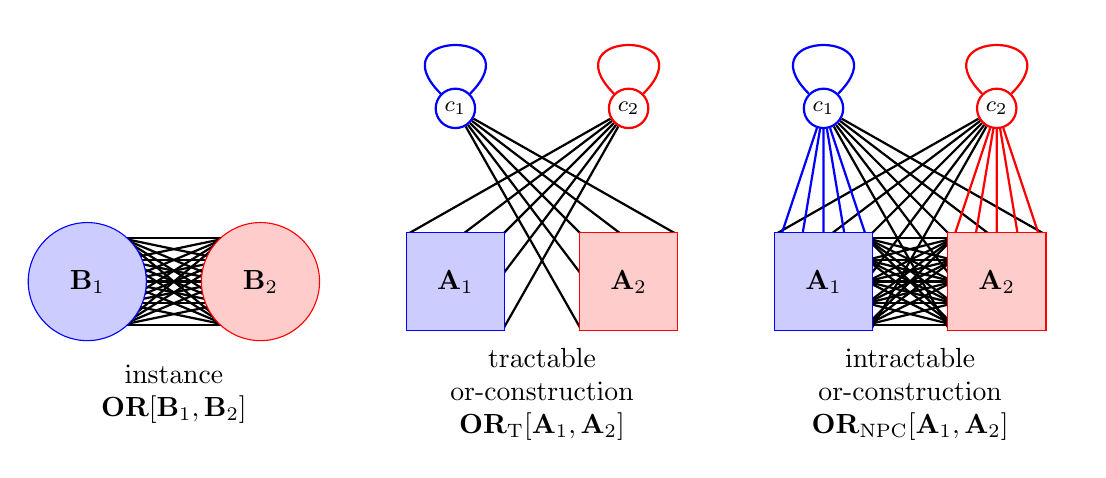
\begin{tikzpicture}[scale=0.55]
			\colorlet{col1}{blue}
			\colorlet{col2}{red}
			\colorlet{colInstance}{red}
			
			\tikzstyle{template1} = [draw=col1, fill=col1!20!white, text=black, rectangle, minimum width=1.25cm, minimum height=1.25cm];
			\tikzstyle{template2} = [draw=col2, fill=col2!20!white, text=black, rectangle, minimum width=1.25cm, minimum height=1.25cm];
			\tikzstyle{instance1} = [draw=col1, fill=col1!20!white, text=black,  circle, minimum width=1.5cm, minimum height=1.5cm];
			\tikzstyle{instance2} = [draw=col2, fill=col2!20!white, text=black,  circle, minimum width=1.5cm, minimum height=1.5cm];
			\tikzstyle{vertex} = [fill=none, minimum width =0.5cm, minimum height = 0.5cm, thick, circle, inner sep = 0mm, font=\footnotesize];
			
			\tikzstyle{sedge} = [black, thick];
			
			\begin{scope}[shift={(-5,0)}]
				\node [instance1] (b1) at (-2,2) {$\StructB_1$};
				\node [instance2] (b2) at (2,2) {$\StructB_2$};
				
				
				\begin{scope}[on background layer]	
					
					\def\ystep{0.5}
					\foreach \i in {-2,...,2}{
						\foreach \j in {-2,...,2} {
							\draw[thick, sedge] ($(b1) + (0.8,\i*\ystep)$) --($(b2) + (-0.8,\j*\ystep)$);
						}
					}
				\end{scope}
				
				\node[text width=3cm, align=center] at (0,-0.6) {instance\\$\OR{\StructB_1,\StructB_2}$};
				
			\end{scope}
			
			
			\def\adstep{0.55}
			\def\avstep{0.5}
			\def\wstep{0.25}
			
			
			
			\begin{scope}[shift = {(3.5,0)}]
				\node [template1, vertex] (c1) at (-2,6) {$c_1$};
				\node [template2, vertex] (c2) at (2,6) {$c_2$};
				\node [template1] (a1) at (-2,2) {$\StructA_1$};
				\node [template2] (a2) at (2,2) {$\StructA_2$};
				
				
				\begin{scope}[on background layer, every loop/.style={}]
					
					\foreach \i in {-2,...,2}{
						\draw[thick, sedge] ($(a1.center) + (\i*\adstep,-\i*\adstep)$) --(c2);
						\draw[thick, sedge] ($(a2) + (\i*\adstep,\i*\adstep)$) --(c1);
					}
					
					
					\draw [thick, col1] (c1) edge [loop] (c1);
					\draw [thick, col2] (c2) edge [loop] (c2);
				\end{scope}
				
				\node[text width=3cm, align=center] at (0,-0.6) {tractable\\ or-construction\\$\ORT{\StructA_1,\StructA_2}$};
			\end{scope}
			
			\begin{scope}[shift = {(12,0)}]
				\node [template1, vertex] (c1) at (-2,6) {$c_1$};
				\node [template2, vertex] (c2) at (2,6) {$c_2$};
				\node [template1] (a1) at (-2,2) {$\StructA_1$};
				\node [template2] (a2) at (2,2) {$\StructA_2$};
				
				
				\begin{scope}[on background layer, every loop/.style={}]
					
					\foreach \i in {-2,...,2}{
						\draw[thick, sedge] ($(a1.center) + (\i*\adstep,-\i*\adstep)$) --(c2);
						\draw[thick, sedge] ($(a2) + (\i*\adstep,\i*\adstep)$) --(c1);
					}
					
					
					\foreach \i in {-2,...,2}{
						\foreach \j in {-2,...,2} {
							\draw[thick, sedge] ($(a2) + (-1,\i*\avstep)$) --($(a1) + (1,\j*\avstep)$);
						}
					}
					
					\foreach \i in {-2,...,2}{
						\draw[thick, col1] ($(a1) + (\i*\avstep,1)$) --(c1);
						\draw[thick, col2] ($(a2) + (\i*\avstep,1)$) --(c2);
					}
					
					\draw [thick, col1] (c1) edge [loop] (c1);
					\draw [thick, col2] (c2) edge [loop] (c2);
				\end{scope}
				\node[text width=3cm, align=center] at (0,-0.6) {intractable or-construction\\$\ORNPC{\StructA_1,\StructA_2}$};
			\end{scope}
		\end{tikzpicture}
		\caption{The different homomorphism or-constructions:
			The picture assumes that the two vocabularies $\sig_1$ and $\sig_2$
			are binary and contain a single relation each (blue and red).
			It shows the instance $\OR{\StructB_1,\StructB_2}$.
			and the tractable and intractable template construction.
			The new $S$-relation is drawn in black,
			where the edges are all oriented from left to right.
			Pairs added to the relation of $\sig_1$ or $\sig_2$
			are drawn in blue or red, respectively.
			\label{fig:hom-or-construction-light}
		}
	\end{figure}
	
	\subparagraph{The Tractable Case.}
	The first variant of the template will preserve tractability of the $\CSP{\StructA_i}$ and is called the \defining{tractable homomorphism or-construction}.
	The template  $\StructA = \ORT{\StructA_1,\StructA_2}$
	is defined as follows.
	Let $c_1$ and $c_2$ be two fresh vertices.
	\begin{align*}
		A &:= A_1 \cup A_2 \cup \set{c_1,c_2}\\
		R^\StructA & :=R^{\StructA_i}  \cup   \set{c_i}^{\arity{R}} & \text{for all } i \in [2], R \in \sig_i\\
		S^\StructA & :=  \big( A_1 \times \set{c_{2}}\big) \cup \big( \set{c_1} \times A_2 \big)
	\end{align*}
	The construction is depicted in Figure~\ref{fig:hom-or-construction-light}.
	Intuitively, a homomorphism $\StructB_i \to \StructA_i$
	induces a homomorphism $\StructB \to \StructA$
	by mapping all vertices of $\StructB_{3-i}$ to $c_{3-i}$.
	The relation $S$ ensures that every homomorphism of $\StructB\to \StructA$
	is of this form, which proves the following lemma:
	\begin{lemma}
		\label{lem:tractable-hom-or-construction-correct}
		$\OR{\StructB_1,\StructB_2} \in \CSP{\ORT{\StructA_1,\StructA_2}}$
		if and only if 
		$\StructB_i \in \CSP{\StructA_i}$ for some $i\in[2]$.
	\end{lemma}
	
	\noindent  The next lemmas summarize the properties of the construction,
	which are required later (full proofs are provided in Appendix~\ref{app:tractable-or}):
	the tractable homomorpism or-construction
	preserves $k$-consistency of the $\StructB_i$
	and inherits solutions of the width-$k$ affine relations from the $\StructB_i$.
	
	
	\begin{lemma}[restate = homOrTractableKConsistency, name = ]
		\label{lem:hom-or-tractable-k-consistency}
		Let $\StructA=\ORT{\StructA_1,\StructA_2}$, $\StructB = \OR{\StructB_1,\StructB_2}$,
		$k \in \nat$, $i\in [2]$, $X \in \tbinom{B}{\leq k}$,
		and $f \in \Hom{\StructB[X]}{\StructA}$.
		If $f(X\cap B_{3-i}) = \set{c_{3-i}}$ and
		$\restrict{f}{X\cap B_i} \in \kcol{k}{\StructA_i}{\StructB_i}(X\cap B_i)$,
		then $f \in \kcol{k}{\StructA}{\StructB}(X)$.
	\end{lemma}
	\begin{lemma}[restate = homOrTractableSolution, name = ]
		\label{lem:hom-or-tractable-solution}
		Let $\StructA=\ORT{\StructA_1,\StructA_2}$, $\StructB = \OR{\StructB_1,\StructB_2}$, 
		$i \in [2]$, and $\Phi$ be a solution to $\cspiso{k}{\StructA_i}{\StructB_i}$.
		Then there is a solution $\Psi$ to $\cspiso{k}{\StructA}{\StructB}$
		defined, for every $X \in \tbinom{B}{\leq k}$
		and $f \in \Hom{\StructB[X]}{\StructA}$,
		by $\Psi(x_{X,f}) = \Phi(x_{X\cap B_i}, \restrict{f}{X\cap B_i})$ if  $f(X \cap B_{3-i}) = \set{c_{3-i}}$
		and $\Psi(x_{X,f}) = 0$ otherwise.
		In particular, $\Psi$ is a $p$-solution or integral,
		if $\Phi$ is a $p$-solution or integral, respectively.
	\end{lemma}
	


	\begin{lemma}[restate = maltsevForOrConstruction, name = ]
		\label{lem:maltsevForOrConstruction}
		If $\StructA_1$ and $\StructA_2$ have a Maltsev polymorphism, then $\ORT{\StructA_1,\StructA_2}$ has one.
	\end{lemma}	
	
	\noindent Also if the $\StructA_i$ are not Maltsev, tractability is preserved.
	\begin{lemma}[restate = homOrTractable, name = ]
		\label{lem:hom-or-tractable}
		If $\CSP{\StructA_1}$ and $\CSP{\StructA_2}$ are tractable, then $\CSP{\ORT{\StructA_1,\StructA_2}}$ is tractable.
	\end{lemma}
	For the case that both $\StructA_i$ are tractable,
	we provide a polynomial-time algorithm for $\CSP{\ORT{\StructA_1,\StructA_2}}$ in Appendix~\ref{app:homomorphism-or}.
	Roughly speaking, the algorithm proceeds as follows:
	If the instance $\StructB$ has connected components, they can be treated individually.
	So we can assume that $\StructB$ is connected.
	The algorithm divides the universe~$B$
	into two sets~$B_1$ and~$B_2$ such that elements in~$B_i$ are contained in tuples of a $\sig_i$-relation. If one is contained in both a $\sig_1$- and a $\sig_2$-relation,
	then~$\StructB$ is a no-instance.
	Because $\StructB$ is connected,~$B_1$ and~$B_2$ are connected by the relation~$S$ (not necessarily by a biclique). By the construction of the tractable or-construction, for any potential homomorphism there is an $i\in[2]$ such that $B_i$ is mapped to $c_i$ and $B_{3-i}$ to $\StructA_{3-i}$.
	This can be tested by the algorithms for $\CSP{\StructA_1}$ and $\CSP{\StructA_2}$.
	Note that this algorithm essentially only computes connected components and calls the decision algorithms of the  $\CSP{\StructA_i}$.
	Hence, it can be expressed in logics that are at least expressive as IFP.
	\begin{corollary}[restate = homOrDefinable, name = ]
		\label{cor:hom-or-definable}
		Let $L$ be a logic that is at least expressive as inflationary fixed-point logic.
		If $\CSP{\StructA_1}$ and $\CSP{\StructA_2}$ are $L$-definable,
		then $\CSP{\ORT{\StructA_1,\StructA_2}}$ is $L$-definable.
	\end{corollary}
	
	\noindent
	The tractable homomorphism or-construction has a drawback:
	forbidding a single partial homomorphism
	mapping vertices of $\StructB_i$ to $c_i$
	resolves the or-construction for the width-$k$ affine relaxation:
	every such solution to the width-$k$ affine relaxation of $\ORT{\StructB_1,\StructB_2}$
	induces a solution for $\StructB_{i}$. 
	
	\begin{lemma}[restate = integerSolutionWithLocalFixingSolvesBi, name = ]
		\label{lem:integerSolutionWithLocalFixingSolvesBi}
		Let $k \geq 2$, $i \in [2]$, 
		and $\Phi$ be a solution to $\cspiso{\StructA}{k+1}{\StructB}$.
		If there is a set $X\in \tbinom{B_i}{\leq k}$ such that
		for $f \colon X \to \set{c_i}$ it holds that
		$\Phi(x_{X,f}) = 0$,
		then $\restrict{\Phi}{B_i}$ is a solution to $\cspiso{\StructA_i}{k}{\StructB_i}$.
	\end{lemma}
	
	\noindent
	In some situations this will cause problems later.
	To remedy this problem,
	we make the construction more flexible at the cost
	of giving up tractability.
	
	
	
	\subparagraph{The Intractable Case.}
	
	The second variant, which is called the \defining{intractable homomorphism or-construction},
	$\StructA = \ORNPC{\StructA_1,\StructA_2}$
	has the same universe as before, but interprets relations differently:
	\begin{align*}
		R^\StructA & :=R^{\StructA_i}  \cup 
		\Big( (A_i \cup \set{c_i})^{\arity{R}} \setminus A_i^{\arity{R}}\Big)
		& \text{for all } i \in [2], R \in \sig_i\\
		S^\StructA & :=  \big( A_1 \times (A_2 \cup \set{c_{2}})\big) \cup \big((A_1 \cup \set{c_{1}} \times A_2\big)
	\end{align*}
	The construction is shown in Figure~\ref{fig:hom-or-construction-light}.
	The definition of $S$ still enforces that a homomorphism 
	$\StructB\to\StructA$ has to induce a homomorphism $\StructB_i\to\StructA_i$
	for one $i$. Only for one $i$, the extra vertex $c_i$ can be in the image of a homomorphism.
	Thus, this variant provides again a homomorphism-or construction,
	but now two \emph{partial} homomorphisms
	$\StructB_1 \to \StructA_1$ and $\StructB_2 \to \StructA_2$
	can be combined:
	
	\begin{lemma}[restate = homOrIntractableCompose, name = ]
		\label{lem:hom-or-intractable-compose}
		Let $\StructA=\ORNPC{\StructA_1,\StructA_2}$,
		$\StructB = \OR{\StructB_1,\StructB_2}$,
		$X_i \subseteq B_i$, and $f_i \in \Hom{\StructB_i}{\StructA_i}$ for both $i\in[2]$.
		The map $f\colon X_1\cup X_2 \to A$ induced by $f_1$ and $f_2$
		satisfies $f \in \Hom{\StructB[X_1\cup X_2]}{\StructA}$.
	\end{lemma}
	
	\noindent Also the intractable construction inherits solutions of the width-$k$ affine relaxation and preserves $k$\nobreakdash-consistency similar to  Lemmas~\ref{lem:hom-or-tractable-k-consistency}
	and~\ref{lem:hom-or-tractable-solution}, but now for the combined partial homomorphisms.
	Instead of  requiring that $f(X \cap B_{3-i}) = \set{c_{3-i}}$,
	we only need  $\restrict{f}{X \cap B_{3-i}} \in \Hom{\StructB_{3-i}[X]}{{\StructA[A_{3-i} \cup \set{c_{3-i}}]}}$  (proofs in Appendix~\ref{app:intractable-or}). 
	Already for easy templates
	the CSP of the intractable homomor\-phism-or construction is NP-complete.
	The reason is that for general instances the $S$-relation does not have to be a biclique and hence a yes-instance does not have to induce a homomorphism for one $\StructB_i$ at all.
	Even for choosing $\StructA_1$ and $\StructA_2$
	to be the structure with a single element and one nonempty ternary relation, the intractable OR-construction yields an NP-complete CSP (e.g.~shown by a reduction from $3$-SAT).
	Many other CSPs can be reduced to this case, for example group-coset-CSPs (full proofs in
	Appendix~\ref{app:intractable-or}).
	
	
	
	
	
	\newcommand{\grpCSP}[3]{\mathcal{C}^{#1,#2,#3}}
	\newcommand{\grpCSPf}[3]{\mathcal{C}^{#3}}
	\newcommand{\egrpCSP}[4]{\mathcal{C}^{#1,#2,#3}_{#4}}
	\newcommand{\egrpCSPf}[4]{\mathcal{C}^{#3}_{#4}}
	
	
	
	\section{Tseitin Formulas over Abelian Groups and Expanders}
	\label{sec:tseitin}
	A family of $2$-connected $3$-regular graphs $(G_n)_{n \in \bbN}$ is a family of \defining{expander graphs} if there is a constant $c > 0$ (the \defining{expansion constant}) such that for all $G_n$ and $X \subseteq E(G_n)$, there is a set $\hat{X} \supseteq X$ of size $|\hat{X}| \leq c|X|$ such that $E(G) \setminus \hat{X}$ is empty or the edge set of a $2$-connected subgraph of~$G$.
	The existence of such families is folklore, see e.g.\ \cite{berkholzGrohe2016fullVersion}.
	Let $G$ be a $2$-connected $3$-regular expander graph.
	Fix an orientation $H$ of $G$, i.e., a directed graph
	with one direction of each edge of $G$. Let $V:= V(G), E := E(G)$ in this section.
	For a set $W \subseteq V$, denote by $\delta_-(W) \subseteq E$
	the set of all $uv\in E$
	such that $(u,v) \in E(H) \cap (V \setminus W) \times W$.
	Analogously, $\delta_+(W)\subseteq E$ is the set of all edges leaving $W$, and $\delta(W) := \delta_+(W) \cup \delta_{-}(W)$.
	Fix a finite Abelian group $\Gamma$. Let $\lambda \colon V \to \Gamma$.
	Define the $\Gamma$-coset-CSP $\grpCSP{H}{\Gamma}{\lambda}$, or $\grpCSPf{H}{\Gamma}{\lambda}$ for short, with variable set $\setcond{y_e }{ e \in E}$ and linear equations
	\begin{align*}
		\sum_{e\in \delta_+(v)} y_e - 	\sum_{e\in \delta_-(v)} y_e &= \lambda(v) &\text{for all } v\in V.
	\end{align*}
	In the case $\Gamma = \ZZ_2$, we obtain the classic Tseitin contradictions~\cite{Tseitin1983}.
The CSP $\grpCSPf{H}{\Gamma}{\lambda}$ is solvable if and only if $\sum_{v \in V} \lambda(v) = 0$ \cite{BerkholzGrohe2017}.
For all sets $W \subseteq V$,
	the CSP $\grpCSPf{H}{\Gamma}{\lambda}$ implies the constraint $C(W)$ defined via
	\[ \sum_{e\in \delta_+(W)} y_e - 	\sum_{e\in \delta_-(W)} y_e = \sum_{v \in W}\lambda(v).\]
	
	
	\begin{definition}[Robustly Consistent Assignments~\cite{BerkholzGrohe2017}]
		For $\lambda \colon V \to \Gamma$ and a set $X \subseteq E$, 
		a partial assignment $f \colon X \to \Gamma$ for $\grpCSPf{H}{\Gamma}{\lambda}$ is \defining{$\ell$\nobreakdash-consistent},
		if for every $W \in \binom{V}{\leq \ell}$ such that $\delta(W) \subseteq X$, the assignment~$f$ satisfies the constraint $C(W)$.
		Note that $f$ is a partial solution if it is $1$-consistent.
		We call $f$ \defining{robustly consistent} if it is $n/3$-consistent.
	\end{definition}
	\noindent We review facts about robustly consistent assignments for $\grpCSPf{H}{\Gamma}{\lambda}$. The detailed statements and proofs can be found in Appendix~\ref{app:tseitin} and~\cite{BerkholzGrohe2017}. The key idea is that the expansion property of~$G$ ensures that $\grpCSPf{H}{\Gamma}{\lambda}$ is always locally satisfiable, on subinstances of size up to $k = o(|E|)$.
	This is because the inconsistency can be ``shifted around'' the graph to any equation outside of the local scope. 
	Thus, for every set~$X$ of at most~$k$ variables, there is at least one robustly consistent assignment with domain~$X$. Robustly consistent assignments are also not discarded by the $k$-consistency procedure. 
	In particular, $k$-consistency always accepts $\grpCSPf{H}{\Gamma}{\lambda}$ even if it has no solution. 
	\begin{lemma}[\cite{BerkholzGrohe2017}]
		\label{lem:group-csp-p-solution}
		If $k \in o(|E|)$ and
		$\Gamma$ is a $p$-group (i.e., $|\Gamma|$ is a power of $p$),
		and ${\lambda \colon V \to \Gamma}$,
		then there is a $p$-solution of $\cspiso{k}{\CosetGrpTmplt{\Gamma}{3}}{\grpCSPf{H}{\Gamma}{\lambda}}$ such that non-robustly consistent partial assignments are set to $0$,
		and each robustly consistent partial solution is mapped to $1/p^\ell$ for some $\ell \in \nat$.
	\end{lemma}
	\noindent The above lemma can also be refined so that the resulting $p$-solution assigns the value $1$ to $x_{X,f}$ for a single robustly consistent partial homomorphism $f\colon X \to \Gamma$ of our choice. 
	
	
	
	
	
	
	
	
	
	
	
	
	
	
	
	\begin{comment}
		\subsection{Extended Tseitin CSP}
		Now also fix a map $\lambda \colon V \to \Gamma$. 
		We now turn the $\Gamma$-CSP $\grpCSPf{H}{\Gamma}{\lambda}$ into 
		a $2$-extended $\Gamma$-CSP.
		We fix an arbitrary vertex $v^* \in V$, introduce a special variable $y^*$,
		and let $\Delta\subseteq \Gamma$ be an arbitrary $2$-element set.
		We define the CSP $\egrpCSP{H}{\Gamma}{\lambda}{\Delta}$
		by replacing the equation for $v^*$ with
		\begin{align*}
			\sum_{e\in \delta_+(v)} y_e - 	\sum_{e\in \delta_-(v)} y_e &= y^*\\
			\intertext{and adding the non-$\Gamma$-constraint}
			y^* &\in\Delta.
		\end{align*} 
		Note that the new constraint increased the arity of the CSP by one to $4$.
		We set $E^* := E \cup \set{y^*}$.
		Again, we will write $\egrpCSPf{H}{\Gamma}{\lambda}{\Delta}$ for $\egrpCSP{H}{\Gamma}{\lambda}{\Delta}$ in this section.
		Recall that when we encode this extended CSP $\StructC := \egrpCSPf{H}{\Gamma}{\lambda}{\Delta}$ as an instance of bounded color class size graph isomorphism, we obtain different pairs of CFI graphs $(\CFIA{\Gamma}{\StructC_\delta}, \CFIB{\Gamma}{\StructC_\delta})$ for all possible values $\delta$ of $y^*$
		(note that $\StructC_\delta = \egrpCSPf{H}{\Gamma}{\lambda}{\set{\delta}}$), and then apply the graph isomorphism or-construction to these. The resulting CSP is $\StructL := \bcisosys{\eCFIA{\Gamma}{\StructC}}{\eCFIB{\Gamma}{\StructC}}$.
		
		So far, the notion of robust consistency has been used for partial solutions of $\grpCSPf{H}{\Gamma}{\lambda}$. We also want to speak about robustly consistent partial solutions of the extended group CSP $\StructC = \egrpCSPf{H}{\Gamma}{\lambda}{\Delta}$ and of the corresponding graph isomorphism CSP $\StructL$.
		
		\begin{definition}[Robustly Consistent Assignments for Extended Group-CSPs]
			For a set $X \subseteq E^*$,
			a partial assignment $f \colon X \to \Gamma$  is \defining{robustly consistent}
			for~$\StructC$
			\begin{enumerate}
				\item if $y^* \in X$ and $f$ is robustly consistent for the group CSP instance $\StructC_\delta$ where $\delta = f(y^*)$, or
				\item if $y^* \notin X$ and, for some $\delta \in \Delta$,
				the assignment $f$ can be extended to $f(y^*) = \delta$ such that it is robustly consistent for $\StructC_\delta$. 
			\end{enumerate}
		\end{definition}
		\begin{definition}[Robustly Consistent Partial Homomorphisms of the GI-CSP]
			~\\
			If $g \in \Hom{\StructL[Y]}{\SymStruct{d}{2}}$ is a partial homomorphism of the graph isomorphism CSP $\StructL$
			that has a \emph{corresponding} partial homomorphism $f \in \Hom{\StructC_\delta[Z]}{\CosetGrpTmplt{\Gamma}{r}}$ for some $\delta \in \Delta$,
			then $g$ is \defining{robustly consistent with respect to $\delta$} if $f$ is robustly consistent.
			Otherwise, $g$ is not robustly consistent.	
		\end{definition}
		
		
		\noindent From now on, we consider extended group-CSP instances
		over  a direct product $\Gamma = \Gamma_1 \times \Gamma_2$ where each $\Gamma_i$ is a $p_i$\nobreakdash-group, for two coprime numbers $p_1$ and $p_2$.
		The non\nobreakdash-$\Gamma$\nobreakdash-constraint is defined in such a way that $\Delta = \{ \delta_1, \delta_2  \}$, where each $\delta_i$ is zero in the $\Gamma_j$ entry, for the $j \neq i$.


	\end{comment}
	
	
	\begin{comment}
		\begin{lemma}[\cite{BerkholzGrohe2017}]
			\label{lem:group-csp-integral-solution}
			Let $n$ be sufficiently larger than $k$,
			$G$ be a $3$-regular and $2$-connected expander,
			$\Gamma_1$ and $\Gamma_2$ be abelian groups, and each $\Gamma_i$ be a $p_i$-group for coprime numbers $p_1$ and $p_2$.
			Set $\Gamma := \Gamma_1\times\Gamma_2$ and $\Delta := \set{(1,0),(0,1)}$.
			Let $\StructA := \egrpCSP{H}{\Gamma_1\times \Gamma_2}{0}{\Delta}$, and $\StructA_{(1,0)}$ and $\StructA_{(0,1)}$ denote the group CSPs obtained from $\StructA$ when the non-group constraint $x^* \in \Delta$ is replaced with $x^* = (1,0)$ or $x^* = (0,1)$, respectively.
			Then the system $\cspiso{k}{\Gamma_4}{\StructA_{(1,0)}}$ has a $p_1$-solution, and  $\cspiso{k}{\Gamma_4}{\StructA_{(0,1)}}$ has a $p_2$-solution.
			These solutions are zero on all non-robustly consistent partial assignments.
		\end{lemma}
	\end{comment}
	
	\begin{comment}
		\begin{lemma}
			\label{lem:k-consistency-group-csp}
			The $k$-consistency algorithm does not rule out any robustly consistent partial solutions of $\egrpCSPf{H}{\Gamma}{\lambda}{\Delta}$.
			This means that, for every $X \in \binom{E^*}{\leq k}$, every robustly consistent homomorphism 
			contained in $\Hom{\egrpCSPf{H}{\Gamma}{\lambda}{\Delta}[X]}{\CosetGrpTmplt{\Gamma}{4}^*}$
			is contained in $\kcol{k}{\CosetGrpTmplt{\Gamma}{4}^*}{\egrpCSPf{H}{\Gamma}{\lambda}{\Delta}} (X)$.
		\end{lemma}
		\begin{proof}
			As in the proof of Lemma \ref{lem:robustlyConsistentSurviveKconsistency},
			let $\Hom{\egrpCSPf{H}{\Gamma}{\lambda}{\Delta}[X]}{\CosetGrpTmplt{\Gamma}{4}^*}_{n/3}$ denote the robustly consistent homomorphisms in $\Hom{\egrpCSPf{H}{\Gamma}{\lambda}{\Delta}[X]}{\CosetGrpTmplt{\Gamma}{4}^*}$. 
			Again we show that the collection 
			\[\setcond*{ \Hom{\egrpCSPf{H}{\Gamma}{\lambda}{\Delta}[X]}{\CosetGrpTmplt{\Gamma}{4}^*}_{n/3}}{X \in \tbinom{E}{\leq k} }\]
			of robustly consistent partial homomorphisms satisfies the down-closure and the forth-condition of $k$-consistency.
			For the down-closure, let $f \in \Hom{\egrpCSPf{H}{\Gamma}{\lambda}{\Delta}[X]}{\CosetGrpTmplt{\Gamma}{4}^*}_{n/3}$.
			Suppose first that $f$ is defined on $y^*$. Then for every subset $Y \subseteq X$ that includes $y^*$, it is immediate that $\restrict{f}{Y} \in \Hom{\egrpCSPf{H}{\Gamma}{\lambda}{\Delta}[X]}{\CosetGrpTmplt{\Gamma}{4}^*}_{n/3}$, just like in Lemma \ref{lem:robustlyConsistentSurviveKconsistency}. If $Y$ does not include $y^*$, then
			$\restrict{f}{Y \cup \{y^*\}}$ is a restriction of the robustly consistent partial homomorphism $f$, and thus is itself robustly consistent. So $\restrict{f}{Y}$ can be extended to $y^*$ to a robustly consistent partial solution; by our definition of robust consistency for $\egrpCSPf{H}{\Gamma}{\lambda}{\Delta}$, this means that $\restrict{f}{Y}$ is robustly consistent. 
			For the forth-condition, let $f \in \Hom{\egrpCSPf{H}{\Gamma}{\lambda}{\Delta}[X]}{\CosetGrpTmplt{\Gamma}{4}^*}_{n/3}$, for some $|X| < k$. Let $y \in E \setminus X$. We need to show that there exists an $f' \in  \Hom{\egrpCSPf{H}{\Gamma}{\lambda}{\Delta}[X \cup \set{y}]}{\CosetGrpTmplt{\Gamma}{4}^*}_{n/3}$ that extends $f$. 
			If $y^* \in X$, then this works exactly as in the proof of Lemma  \ref{lem:robustlyConsistentSurviveKconsistency}. If $y^* \notin X$, then by our definition of robust consistency, there is some $\delta \in \Delta$ such that $f$ is robustly consistent for $\StructC_\delta$. Suppose first that $y \neq y^*$. Then we know with the same argument as in the proof of Lemma \ref{lem:robustlyConsistentSurviveKconsistency} that there exists an $f' \in  \Hom{\egrpCSPf{H}{\Gamma}{\lambda[v^*\mapsto \delta]}{\Delta}[X \cup \set{y}]}{\CosetGrpTmplt{\Gamma}{4}^*}_{n/3}$. Hence, $f'$ is robustly consistent as witnessed by this choice of $\delta \in \Delta$. In the case that $y = y^*$, we set $f'(y^*) = \delta$. This is robustly consistent by definition. 
		\end{proof}
		
		
		\begin{corollary}
			\label{cor:kConsistencyFailsOnDeltaConstraints}
			For all $X \in \binom{E^*}{\leq k}$,
			we have  $\kcol{k}{\CosetGrpTmplt{\Gamma}{4}^*}{\egrpCSPf{H}{\Gamma}{\lambda}{\Delta}}(X) \neq \emptyset$.
		\end{corollary}	
		\begin{proof}
			By Lemma \ref{lem:k-consistency-group-csp}, robustly consistent partial solutions survive $k$-consistency. It remains to argue that for every $X \in \binom{E^*}{\leq k}$, there is a robustly consistent assignment with domain~$X$. But this follows immediately from Lemma \ref{lem:robustly-consistent-for-all-small-contexts} because it holds for every $\lambda$; so in particular for every $\delta \in \Delta$ that can be assigned to $y^*$. 
		\end{proof}	
		
		\noindent We now need to consider the case when one robustly consistent partial solution is fixed.
		We show that in this case
		the system $\cspiso{k}{\SymStruct{d}{2}}{\StructL}$ has still an integral solution.
		Let $Y \subseteq \binom{E^*}{\leq k}$
		and $\hat{g} \in \Hom{\StructL[Y]}{\SymStruct{d}{2}}$ be robustly consistent with respect to some $\delta \in \Delta$.
		This is the partial solution that we want to treat as fixed.
		Let $\hat{f} \in \Hom{\StructC_\delta[Z]}{\CosetGrpTmplt{\Gamma}{4}}$ be the corresponding partial solution of $\StructC_\delta$. 
		Fix a set $\hat{Z} \supseteq Z$ such that $E \setminus \hat{Z}$ is the edge set of a $2$-connected subgraph of $G$.
		By the expansion property, we can choose it such that $|\hat{Z}| \leq c \cdot |Z|$, where $c$ is the expansion constant. 
		\begin{lemma}
			\label{lem:fHatCanBeExtended}
			There is an assignment $\hat{h} : \hat{Z} \to \Gamma$ such that $\hat{h}|_{Z} = \hat{f}$, and $\hat{h} \in \Hom{\StructC_\delta[\hat{Z}]}{\CosetGrpTmplt{\Gamma}{3}}$ is robustly consistent.
		\end{lemma}	
		\begin{proof}
			Since $|\hat{Z}| \leq c \cdot |Z| \leq c \cdot 4 \cdot |Y| = 4ck$, we can use Lemmas 4.4 and 4.5 in \cite{BerkholzGrohe2017} to extend~$\hat{f}$ to a robustly consistent~$\hat{h}$ with domain $\hat{Z}$. This is in particular a partial solution.
		\end{proof}	
		\noindent Fix this partial solution $\hat{h} \colon \hat{Z} \to \Gamma$ 
		for $\StructC_\delta$ given by Lemma~\ref{lem:fHatCanBeExtended} in the following.
		Let $G'=(V',E')$ be the graph obtained from $G$ by deleting all edges in $\hat{Z}$
		and all vertices that are not in the $2$-connected component of $G-\hat{Z}$.
		Similarly, obtain the directed graph $H'$ from $H$ by deleting the same (directed) edges and vertices.
		Let $\lambda' : V' \to \Gamma$ be defined as follows. For every $v \in V'$, set
		\[
		\lambda'(v) := \lambda(v) - \sum_{e \in \delta_+(v) \cap \hat{Z}} \hat{h}(y_e) + \sum_{e \in \delta_-(v) \cap \hat{Z}} \hat{h}(y_e) .
		\] 
		With this definition, $\grpCSP{H'}{\Gamma}{\lambda'}$ is the CSP that we obtain from $\StructC_\delta$ by fixing values for the variables in $\hat{Z}$ according to $\hat{h}$ from Lemma \ref{lem:fHatCanBeExtended}.
		\begin{lemma}
			\label{lem:piecingTogetherPhiAndSolution}
			Let $\StructC_\delta = \egrpCSP{H}{\Gamma}{\lambda}{\set{\delta}}$
			and $\StructC' = \grpCSP{H'}{\Gamma}{\lambda'}$.
			If $\cspiso{4k}{\CosetGrpTmplt{\Gamma}{4}}{\StructC'}$ has a $p$-solution $\Phi$, then $\cspiso{4k}{\CosetGrpTmplt{\Gamma}{4}}{\StructC_\delta}$ has a $p$-solution $\Psi$ such that
			\begin{enumerate}
				\item if $\Phi(e) = 0$, then $\Psi(e) = 0$, for every $e \in E'$, and
				\item  for all sets of variables $X \in \binom{E \setminus E'}{\leq 4k}$ of the system $\StructC_\delta$ and for all partial homomorphisms $f \in \Hom{\StructC_\delta[X]}{\CosetGrpTmplt{\Gamma}{4}}$,
				we have $\Psi(y_{X,f}) = 1$ if $f$ agrees with $\hat{h}$, and $\Psi(y_{X,f}) = 0$, otherwise.
			\end{enumerate}
		\end{lemma}	
		\begin{proof}
			Define $\Psi$ as follows. Let $\StructC' = \grpCSP{H'}{\Gamma}{\lambda'}$
			with variables $E'$. For all $X \in \binom{E}{\leq k}$ and $f \in \Hom{\StructC_\delta[X]}{\CosetGrpTmplt{\Gamma}{4}}$, we have
			\[
			\Psi(x_{X,f}) := \begin{cases}
				\Phi(x_{X \cap E',f|_{E'}}) & \text{ if } f|_{X \setminus E'} = \hat{h}|_{X \setminus E'} \text{ or if } X \subseteq E',\\
				0 & \text{ otherwise.}
			\end{cases}
			\]
			It remains to show that $\Psi$ is a solution for $\cspiso{4k}{\CosetGrpTmplt{\Gamma}{4}}{\StructC_\delta}$.
			For Equation~\ref{eqn:csp-iso-empty}, this is clear. Now consider equation of Type~\ref{eqn:csp-iso-agree}:
			Let $X \in \binom{E}{\leq k}$, $b \in X$, and $g \in \Hom{\StructC_\delta}{\CosetGrpTmplt{\Gamma}{4}}$.
			We need to show 
			\[\sum_{\substack{f \in \Hom{\StructC_\delta[X]}{\CosetGrpTmplt{\Gamma}{4}},\\ \restrict{f}{X\setminus\set{b}} = g}} \Psi(x_{X,f}) =  \Psi(x_{X\setminus \{b\},g}).\]
			If $g|_{(X \setminus b) \setminus C}$ does not agree with $\hat{h}$, then both sides of the equation are mapped to zero by $\Psi$. Hence it remains the case that $g|_{(X \setminus b) \setminus E'}$ does agree with $\hat{h}$.
			For every $f \in \Hom{\StructC_\delta[X]}{\CosetGrpTmplt{\Gamma}{4}}$, it holds: If $f|_{X \setminus E'} = \hat{h}|_{X \setminus E'}$, then $f|_{E'} \in \Hom{\StructC'[X \cap E']}{\CosetGrpTmplt{\Gamma}{4}}$. This is due to the definition of~$\lambda'$. Thus we have
			\begin{align*}
				\sum_{\substack{f \in \Hom{\StructC_\delta[X]}{\CosetGrpTmplt{\Gamma}{4}},\\ \restrict{f}{X\setminus\set{b}} = g}} \Psi(x_{X,f}) &= \sum_{\substack{f \in \Hom{\StructC'[X \cap E']}{\CosetGrpTmplt{\Gamma}{4}},\\ \restrict{f}{X \cap E' \setminus\set{b}} = g}} \Phi(x_{X \cap E',f|_{E'}})\\
				&= \Phi(x_{(X \cap E')\setminus \{b\},g|_{E'}}) = \Psi(x_{X\setminus \{b\},g}  ).
			\end{align*}	
			Therefore, $\Psi$ is a solution of $\cspiso{4k}{\CosetGrpTmplt{\Gamma}{4}}{\StructC_\delta}$. For every $X \in E \setminus E'$, we have $\Psi(x_{X,f}) = 0$ if $f$ disagrees with $\hat{h}$, and $\Psi(x_{X,f}) = \Phi(x_{X \cap C,f|_{C}}) = \Phi(x_{\emptyset,\emptyset}) = 1$, otherwise.
		\end{proof}	
		
		
		
		\begin{lemma}
			\label{lem:group-csp-p-solution-with-fixed-assignment}
			If $\hat{g} \in \Hom{\StructL[Y]}{\SymStruct{d}{2}}$ is robustly consistent with respect to $\delta_i \in \Delta$, then $\cspiso{k}{\SymStruct{d}{2}}{\StructL}$ has a $p_i$-solution $\Psi$ such that
			\begin{itemize}
				\item $\Psi$ is $0$ for partial assignments that are not robustly consistent with respect to $\delta$, and
				\item $\Psi(x_{Y,\hat{g}}) = 1$.
			\end{itemize}
		\end{lemma}
		\begin{proof}
			Because $\hat{g}$ is robustly consistent with respect to~$\delta$, its corresponding partial solution $\hat{f} \in \Hom{\StructC_\delta[Z]}{\CosetGrpTmplt{\Gamma}{4}}$ is robustly consistent. With Lemma \ref{lem:fHatCanBeExtended}, we extend $f$ to $\Phi \in \Hom{\StructC_\delta[\hat{Z}]}{\CosetGrpTmplt{\Gamma}{4}}$.
			The graph $G'$ is still an expander graph (follows from Lemma \ref{lem:expandersRobust}). Hence
			Lemma \ref{lem:group-csp-p-solution} can be applied and gives us a $p_i$-solution for $\cspiso{k}{\CosetGrpTmplt{\Gamma}{4}}{\StructC'}$, to which we can apply Lemma \ref{lem:piecingTogetherPhiAndSolution} to get a $p_i$-solution for $\cspiso{4k}{\CosetGrpTmplt{\Gamma}{4}}{\StructC_\delta}$.
			This has the property that it is zero for assignments which are not robustly consistent and it is $1$ for $x_{Z,\hat{f}}$.
			To this solution, we apply Lemmas \ref{lem:cfi-p-solution} and \ref{lem:or-construction-p-solution}, yielding the desired solution $\Psi$. 
		\end{proof}	
		
		
	\end{comment}
	
	
	
	\newcommand{\ZtwoOrThreeInst}{\ORT{\CosetGrpTmplt{\ZZ_2}{3}, \CosetGrpTmplt{\ZZ_3}{3}}}
	\section{Limitations of the Affine Algorithms}
	\label{sec:power-of-affine}
	All of the affine algorithms are \emph{sound}: they accept all yes-instances.
	This section shows that many of them are note \emph{complete} on tractable CSPs:  they do not reject all no-instances, and thus do not solve the CSP.
	We consider the tractable homomorphism or-construction $\ORT{\CosetGrpTmplt{\ZZ_2}{3}, \CosetGrpTmplt{\ZZ_3}{3}}$
	of the ternary $\ZZ_2$-coset-CSP and  the ternary $\ZZ_3$-coset-CSP.
	
	
	
	\subsection{\texorpdfstring{$\ZZ$}{ℤ}-Affine \texorpdfstring{$k$}{k}-Consistency Relaxation}
	\label{sec:zAffineConsistency}
	
	
	The \defining{$\ZZ$-affine $k$-consistency relaxation} \cite{DalmauOprsal2024}
	solves the following system of affine linear equations over the integers.
	Let $\StructA$ be a template, $\StructB$ be an instance,
	and $\kappa$ be a map
	assigning to every set  $X \in \binom{B}{\leq k}$ a set of partial homomorphisms $\StructB[X] \to \StructA$.
	Define the system $\zafkleq{k}{\StructA}{\StructB}{\kappa}$:
	
	\begin{systembox}{$\zafkleq{k}{\StructA}{\StructB}{\kappa}$: variables $z_{X,f}$
			for all $X \in {\tbinom{B} {\leq k}}$
			and $f \in \kappa(X)$}
		\begin{align*}
			z_{X,f} &\in \ZZ &  \text{for all } X \in \tbinom{B}{\leq k} \text { and } f \in \kappa(X)\\
			\sum_{f \in \kappa(X)}  z_{X,f}&= 1 &  \text{for all } X \in \tbinom{B}{\leq k}\\
			\sum_{f \in \kappa(X), \restrict{f}{Y} = g} z_{X,f} &= z_{Y,g} & \text{for all } Y\subset X \in \tbinom{B}{\leq k} \text { and } g \in \kappa(Y) 
		\end{align*}
	\end{systembox}
	
	\noindent 
	For a fixed positive integer $k$, a template structure $\StructA$,
	and an instance $\StructB$,
	the $\ZZ$-affine $k$-consistency relaxation runs the $k$-consistency algorithm
	to compute $\kcol{k}{\StructA}{\StructB}$,
	the function that maps each set $X \in \binom{B}{\leq k}$ to the set of $k$-consistent partial homomorphisms $\StructB[X] \to \StructA$.
	The instance $\StructB$ is accepted by the algorithm
	if $\zafkleq{k}{\StructA}{\StructB}{\kcol{k}{\StructA}{\StructB}}$ has an integral solution and rejects $\StructB$ otherwise.
	Dalmau and Opr\v{s}al~\cite{DalmauOprsal2024} conjectured the following
	on the power of the $\ZZ$-affine $k$-consistency relaxation:
	\begin{conjecture}[restate=sthreeorZ, name = \cite{DalmauOprsal2024}]
		\label{con:s3-or-Z}
		For every finite structure $\StructA$,
		either
		$\CSP{K_3}$ is Datalog$^\cup$-reducible to $\CSP{\StructA}$
		or
		$\CSP{\StructA}$ is Datalog$^\cup$-reducible to $\CSP{\ZZ}$,
		where $K_3$ denotes the triangle.
	\end{conjecture}
	\noindent Being Datalog$^\cup$-reducible to $\CSP{\ZZ}$ implies
	that $\CSP{\StructA}$ is solved by $\ZZ$-affine $k$\nobreakdash-consistency for some constant $k$~\cite{DalmauOprsal2024}, which we show is not the case for our counterexample.
	
	
	
	
	\begin{theorem}[restate=zAffineDoesNotSolveBoundedColorClass, name =]
		\label{thm:z-affine-does-not-solve-bounded-color-class}
		For every $k\geq 1$, the $\ZZ$-affine $k$-consistency relaxation does not solve $\ZtwoOrThreeInst$.
		This is even true if $k$ is not a constant, but an at most sublinear function in the instance size.
	\end{theorem}
	
	\begin{proof}\textcolor{red}{TOPROVE 0}\end{proof}
\begin{lemma}[restate=notDatalogReducible, name =]
		\label{lem:not-datalog-reducible}
		$\CSP{K_3}$ is not Datalog$^\cup$-reducible to $\CSP{\ZtwoOrThreeInst}$.
	\end{lemma}
	\noindent
	Theorem~\ref{thm:z-affine-does-not-solve-bounded-color-class}
	and Lemma~\ref{lem:not-datalog-reducible}
	disprove Conjecture~\ref{con:s3-or-Z}.
	To show the lemma, we show that $\CSP{\CosetGrpTmplt{\ZZ_p}{r}}$ is not Datalog$^\cup$-reducible to $\CSP{\ZtwoOrThreeInst}$ for a prime $p \notin\set{2,3}$.
	This suffices because $\CSP{\CosetGrpTmplt{\ZZ_p}{r}}$ is Datalog$^\cup$-reducible to $\CSP{K_3}$~\cite{DalmauOprsal2024}.
	We use results from finite model theory:
	$\set{2,3}$-rank logic~\cite{DawarGHL09}
	extends IFP by a rank operator for definable matrices over~$\ZZ_2$ and~$\ZZ_3$.
	The logic defines $\CSP{\CosetGrpTmplt{\ZZ_2}{3}}$ and $\CSP{\CosetGrpTmplt{\ZZ_3}{3}}$
	and so also $\CSP{\ZtwoOrThreeInst}$ by Corollary~\ref{cor:hom-or-definable}.
	If $\CSP{\CosetGrpTmplt{\ZZ_p}{r}}$ is Datalog$^\cup$-reducible to 
	$\CSP{\ZtwoOrThreeInst}$,  
	then $\set{2,3}$-rank logic solves~$\CSP{\CosetGrpTmplt{\ZZ_p}{r}}$ because IFP expresses Datalog$^\cup$-reductions. But $\ZZ_p$-equation systems are only solvable in $\set{2,3}$-rank logic if $p \in \{2,3\}$~\cite{GradelPakusa19} (full proof in Appendix~\ref{app:zAffineConsistency}).
	
	
	
	
	\newcommand{\BLPAIP}[1]{\mathsf{BLP{+}AIP}(#1)}
	\newcommand{\BAk}[2]{\mathsf{BA}^{#1}(#2)}
	\newcommand{\VarsIP}[3]{\mathcal{V}^{#1,#2}(#3)}
	\subsection{BLP+AIP and BA\texorpdfstring{$^k$}{k}}
	\label{sec:BLP}
	We introduce another well-studied system of equations for CSPs~\cite{BartoBKO2021,BrakensiekGWZ2020} parameterized by the size of partial solutions~\cite{CiardoZivny2023GraphColoring}.
	Let $k$ be a positive integer, $\StructA$ a template $\sig$-structure
	and~$\StructB$ a $\CSP{\StructA}$-instance.
	We define the system
	$\ipk{k}{\StructA}{\StructB}$ with variable set $\VarsIP{k}{\StructA}{\StructB}$.
	
	\begin{systembox}{$\ipk{k}{\StructA}{\StructB}$: 
			variables $\lambda_{X,f}$ for all $X \in \tbinom{B}{\leq k}$ and  $f\colon X \to A$, and \\\phantom{$\ipk{k}{\StructA}{\StructB}$: }variables $\mu_{R,\tup{b},\tup{a}}$ for all $R \in \sig$, $\tup{b} \in R^\StructB$, and $\tup{a} \in R^\StructA$}
		\setlength{\belowdisplayskip}{2pt}
		\begin{align*}
			\sum_{f \colon X \to A} \lambda_{X,f} &= 1  &\text{for all } X \in \tbinom{B}{\leq k},\\
			\sum_{\substack{f \colon X \to A,\\\restrict{f}{Y} = g}} \lambda_{X,f} &= \lambda_{Y,g} & \text{for all } Y\subset X \in \tbinom{B}{\leq k}, g\colon Y \to A,\\
			\sum_{\tup{a} \in R^\StructA, a_{\tup{i}} = \tup{a}'} \mu_{R,\tup{b},\tup{a}} &= \lambda_{X(\tup{b}_{\tup{i}}), \tup{b}_{\tup{i}} \mapsto \tup{a}' } &  \text {for all } R \in \sig, \tup{a}' \in A^k, \tup{b} \in R^\StructB, \tup{i} \in [\arity{R}]^k,
		\end{align*}
	where $a_{\tup{i}}$ and $b_{\tup{i}}$ are the $k$-tuples $(a_{\tup{i}_1},...,a_{\tup{i}_k})$ and $(b_{\tup{i}_1},...,b_{\tup{i}_k})$, respectively, $X(\tup{b}_{\tup{i}})$ is the set of entries of $\tup{b}_{\tup{i}}$, and $\tup{b}_{\tup{i}} \mapsto \tup{a}'$ is the function$ X(\tup{b}_{\tup{i}})\to A$ mapping $\tup{b}_{\tup{i}}$ to $\tup{a}'$.
	\end{systembox}
	\noindent Different domains of the variables (see~\cite{BrakensiekGWZ2020}) are of interest: If we restrict the variables to $\set{0,1}$, then
	$\ipk{1}{\StructA}{\StructB}$ is solvable if and only if
	$\StructB \in \CSP{\StructA}$.
	The relaxation of $\ipk{k}{\StructA}{\StructB}$ to nonnegative rationals is the \defining{$k$-basic linear programming (BLP)} relaxation $\blk{k}{\StructA}{\StructB}$\footnote{The literature~\cite{BrakensiekGWZ2020, CiardoZivny2023BAk} only calls $\blk{1}{\StructA}{\StructB}$ the basic linear programming relaxation. For convenience and uniformity, we extend the notion in this paper to arbitrary $k$.}.
	The affine relaxation of $\ipk{k}{\StructA}{\StructB}$ to all integers is the \defining{$k$-affine integer programming (AIP)} relaxation $\aipk{k}{\StructA}{\StructB}$.
	By increasing the parameter~$k$, 
	the BLP and AIP relaxations result in the Sherali-Adams LP hierarchy~\cite{sherali1990hierarchy} and
	the affine integer programming hierarchy~\cite{CiardoZivny2023GraphColoring} of the $\{0,1\}$-system, respectively.
In contrast to the $\ZZ$-affine $k$-consistency relaxation,
	the BLP+AIP algorithm is not parameterized by the size of partial solutions $k$.
	Ciardo and Živný~\cite{CiardoZivny2023Tensors,  CiardoZivny2023BAk} proposed this parameterized version called \defining{BA$^k$}, where BA$^1$ is just the BLP+AIP algorithm.
	
	\begin{algobox}{$\BAk{k}{\StructA}$-algorithm: input a $\CSP{\StructA}$-instance $\StructB$}
		\begin{enumerate}
			\item Compute a relative interior point $\Phi \colon \VarsIP{k}{\StructA}{\StructB} \to \QQ $ in the polytope defined by $\blk{k}{\StructA}{\StructB}$.
			The solution $\Phi$ has in particular the property that for each variable $x \in \VarsIP{k}{\StructA}{\StructB}$ there is a solution $\Psi$ to $\blp{\StructA}{\StructB}$ such that $\Psi(x) \neq 0$
			if and only if $\Phi(x) \neq 0$.
			If such a point does not exist, reject.\label{itm:short-bak-interior-point}
			\item \label{item:short-bak-refined-constr} Refine $\aipk{k}{\StructA}{\StructB}$ by adding the constraints
			$x = 0$ whenever $\Phi(x) = 0 $ for all $x\in \VarsIP{k}{\StructA}{\StructB}$.
			\item If the refined system is feasible (over $\ZZ$), then accept, otherwise reject.
		\end{enumerate}	
	\end{algobox}
	\noindent The original presentation of BA$^k$~\cite{CiardoZivny2023Tensors} uses a slightly different system of equations but one can easily verify that our presentation is equisatisfiable. The system in \cite{CiardoZivny2023Tensors} does not have variables $\lambda_{X,f}$ but uses variables $\lambda_{R_k,\tup{b},\tup{a}}$ instead, where $R_k$ is the full $k$-ary relation. We deviate from the presentation in \cite{CiardoZivny2023Tensors} to keep it consistent with the systems for the other algorithms.
	We show that BA$^k$ fails on the counterexample provided for $\ZZ$-affine $k$-consistency.
	
	
	\begin{theorem}[restate=BLPDoesNotSolveBoundedColorClass, name=]
		\label{thm:BLP-does-not-solve-bounded-color-class}
		For every integer $k$, the algorithm $\BAk{k}{\StructA}$ does not solve
		$\ZtwoOrThreeInst$. This is even true if $k$ is not a constant but an at most sublinear function in the instance size.
	\end{theorem}
	\noindent The theorem is proved using the same construction as for Theorem~\ref{thm:z-affine-does-not-solve-bounded-color-class}.
	One shows, for~$k$ at least the arity of $\StructA$, that a non-negative or integral solution of $\cspiso{k}{\StructA}{\StructB}$
	implies a solution for $\blk{k}{\StructA}{\StructB}$
	or $\aipk{k}{\StructA}{\StructB}$, respectively.
	The solution to $\blk{k}{\StructA_i}{\StructB_i}$,
	where $\StructB_i$ is the Tseitin-system over $p_i = i+1$,
	is non-zero and non-negative exactly for the robustly consistent partial homomorphisms.
	This carries over to the notion of  robustly consistent partial homomorphisms
	for the or-instance $\StructB = \OR{\StructB_1,\StructB_2}$.
	This implies that the interior point computed in Step~\ref{itm:short-bak-interior-point} is non-zero for robustly consistent partial homomorphisms.
	So they are not set to zero in Step~\ref{item:short-bak-refined-constr}
	and there is an integral solution (full proof in Appendix~\ref{app:BLP}).
	
	
	\subsection{The CLAP Algorithm}
	\label{sec:CLAP}
	The CLAP algorithm~\cite{CiardoZivny2023CLAP} combines the BLP and the AIP relaxation.
	It first iteratively reduces the solution space using BLP by fixing partial solutions to $1$ and discarding those for which this refined BLP is not solvable.
	Then BLP+AIP is run on the restricted solution space, where again a partial solution is fixed:
	
	\begin{algobox}{$\CLAP{\StructA}$-algorithm:
			input a $\CSP{\StructA}$-instance $\StructB$}
		\begin{enumerate}
			\item Maintain, for each relation symbol $R\in \sig$ and  each tuple $\tup{b} \in R^\StructB$,
			a set $S_{\tup{b},R} \subseteq R^\StructA$ of possible images of $\tup{b}$ under a homomorphism.
			Initialize $S_{\tup{b},R} := R^\StructA$. 
			\item Repeat until no set $S_{\tup{b},R}$ changes anymore:
			For each $R\in\sig$, $\tup{b} \in R^\StructB$, and $\tup{a} \in S_{\tup{b},R}$, solve $\blk{1}{\StructA}{\StructB}$ together with the following additional constraints:
			\setlength{\abovedisplayskip}{5pt}
			\setlength{\belowdisplayskip}{5pt}
			\begin{align*}
				\mu_{R,\tup{b},\tup{a}} &= 1,\\
				\mu_{R',\tup{b}',\tup{a}'} &= 0 &\text{for all } R' \in \sig, \tup{b}'\in R'^\StructB, \tup{a}' \not\in S_{\tup{b'},R'}.
			\end{align*}
			If this system is not feasible, remove $\tup{a}$ from $S_{\tup{b},R}$.
			\item If there are $R\in\sig$ and $\tup{b}\in R^\StructB$ such that $S_{\tup{b},R} =\emptyset$, then reject.
			\item For each $R \in \sig$, $\tup{b} \in R^\StructB$, and $\tup{a} \in S_{\tup{b},R}$, execute $\BAk{1}{\StructA}$ (which is BLP+AIP) on~$\StructB$, where we additionally fix
			\begin{align*}
				\mu_{R,\tup{b},\tup{a}} &= 1,\\
				\mu_{R',\tup{b}',\tup{a}'} & = 0 &\text{for all } R' \in \sig, \tup{b}' \in R'^\StructB, \tup{a}' \not\in S_{\tup{b}',R'}
			\end{align*}
			in Step~\ref{itm:bak-interior-point} of $\BAk{1}{\StructA}$.
			If $\BAk{1}{\StructA}$ accepts, then accept.\label{itm:clap-call-bak-short}
			\item If $\BAk{1}{\StructA}$ rejects all inputs in the step before, then reject.
		\end{enumerate}
	\end{algobox}
	
	\noindent Note that the algorithm accepts in Step~\ref{itm:clap-call-bak-short}
	if for \emph{one} $R \in \sig$, one $\tup{b} \in R^\StructB$, and one $\tup{a} \in S_{\tup{b},R}$ BLP+AIP accepts when fixing the partial solution $\tup{b} \mapsto \tup{a}$ (in contrast to the stronger requirement that for each  $R \in \sig$ and $\tup{b} \in R^\StructB$, there is one $\tup{a} \in S_{\tup{b},R}$ for which BLP+AIP accepts).
	We show that this weaker requirement can actually by omitted and
	does not change whether CLAP solves $\CSP{A}$.
	This is crucial to show that CLAP fails on the same counterexample.
	
	\begin{theorem}[restate=clapDoesNotSolveAll, name = ]
		\label{thm:clap-does-not-solve-all}
		$\CLAP{\StructA}$ does not solve $\CSP{\ZtwoOrThreeInst}$.
	\end{theorem}
	\noindent We prove this theorem again with the construction from the proof of Theorem~\ref{thm:z-affine-does-not-solve-bounded-color-class},
	where we pick~$k$ to be the arity of~$\StructA$.
	Again we have to argue that the pruning steps never remove robustly consistent partial homomorphisms.
	Here we also need the property of the Tseitin systems that their relaxation admits a~$p_i$-solution even if we require a given partial homomorphism to receive value~$1$.
	A full proof is provided in Appendix~\ref{app:CLAP}.
	Theorems~\ref{thm:z-affine-does-not-solve-bounded-color-class},~\ref{thm:BLP-does-not-solve-bounded-color-class}, and~\ref{thm:clap-does-not-solve-all}
	\textbf{prove Theorem~\ref{thm:mainResultInformal}}.
	Our arguments do not exploit that CLAP uses $\blk{1}{\StructA}{\StructB}$ and 
	$\BAk{1}{\StructA}$ and is not parametrized by a width~$k$.
	Hence, a parameterized version of CLAP will fail on the same counterexample.
	
	
	
	
	
	\subsection{The Cohomological \texorpdfstring{$k$}{k}-Consistency Algorithm}
	\label{sec:cohomology}
	The cohomological $k$-consistency algorithm due to Ó Conghaile \cite{OConghaile22} was originally presented in categorical and cohomological notions but computing cohomology groups is nothing else than solving a system of linear equations over the integers.
	Therefore, we can state the algorithm in a way similar to the other algorithms seen so far.
	\begin{algobox}{Cohomological $k$-consistency algorithm:
			input a $\CSP{\StructA}$-instance $\StructB$}
		\begin{enumerate}
			\item Maintain, for each $X \in \binom{B}{ \leq k}$, a set $\Hh(X) \subseteq \Hom{\StructB[X]}{\StructA}$. Initialize $\Hh(X) := \Hom{\StructB[X]}{\StructA}$.
			\item Repeat until none of the sets $\Hh(X)$ changes anymore: 
			\begin{enumerate}
				\item Run the $k$-consistency algorithm on $\Hh$ and remove from each $\Hh(X)$ the partial homomorphisms that fail the forth-condition or down-closure property.
				\item For each $X \in \binom{B}{ \leq k}$ and $f \in \Hh(X)$, check whether $\zafkleq{k}{\StructA}{\StructB}{\Hh}$ has a solution that satisfies $x_{X,f} = 1$ and $x_{X,f'} = 0$ for every $f' \in \Hh(X) \setminus \{f\}$. If it does not, then remove $f$ from $\Hh(X)$ for the next iteration of the loop. 
			\end{enumerate}	
			\item If $\Hh(X) = \emptyset$ for some $X \in \binom{B}{\leq k}$, then reject; otherwise accept. 
		\end{enumerate}
	\end{algobox}
	\noindent Step 2(b) of the algorithm approximates whether
	there is a global homomorphism whose restriction to $X$ is equal to $f$
	via solving the $\zafkleq{k}{\StructA}{\StructB}{\Hh}$
	in which we set $x_{X,f} = 1$ and $x_{X,f'} = 0$ for all other~$f'$.
	At least for the template $\CSP{\ZtwoOrThreeInst}$, the  cohomological $k$-consistency algorithm is strictly more powerful than the previous ones because it correctly rejects the instances:
	
	\begin{theorem}[restate=cohomologySolvesCounterexample, name=]
		\label{thm:cohomologySolvesCounterexample}
		If $\StructA_1, \StructA_2$ are templates of Abelian coset-CSPs
		and $k\geq \arity{A_i}+1$ for both $i\in[2]$,
		then the $k$-cohomological algorithm solves $\CSP{\ORT{\StructA_1,\StructA_2}}$.
	\end{theorem}
	\noindent The proof  exploits Lemma~\ref{lem:integerSolutionWithLocalFixingSolvesBi}:
	When a partial homomorphism of $\StructB_i$ is fixed as in Step~2(b) of the algorithm,
	then the tractable homomorphism or-construction is resolved:
	$\zafkleq{k}{\StructA}{\StructB}{\Hh}$ (with the additional constraints)
	has an integral solution only if $\zafkleq{k}{\StructA_i}{\StructB_i}{\Hh}$
	has an integral solution.
	But for Abelian coset-CSPs, $\zafkleq{k}{\StructA_i}{\StructB_i}{\Hh}$ has an integral solution if and only if $\StructB_i \in \CSP{\StructA_i}$ (see Section~\ref{sec:groupStuff}).
	This means that there is no integral solution
	and the algorithm rejects $\StructB$.
	Actually, showing that the cohomological algorithm correctly solves all instances 
	also follows the algorithm for Lemma~\ref{lem:hom-or-tractable} (proofs in Appendix~\ref{app:cohomology}).
	While the algorithm correctly solves the tractable homomorphism or-construction,
	it fails on the \emph{intractable} one. This proves \emph{without} complexity-theoretic assumptions like P $\neq$ NP that this polynomial-time algorithm does not solve all finite-domain CSPs.
	
	\begin{theorem}[restate=cohomologyDoesNotSolveAllCSP, name =]
		\label{thm:cohomologyDoesNotSolveAllCSP}
		There is an NP-complete template structure $\StructA$ such that for every $k$,
		the cohomological $k$-consistency algorithm does not solve $\CSP{\StructA}$.
	\end{theorem}
	\noindent The theorem is proved using the same setup as in the counterexample for the other algorithms, but
	we use the intractable homomorphism or-construction.
	This makes the crucial difference that, by Lemma~\ref{lem:hom-or-intractable-compose},
	two partial homomorphisms of both $\StructB_1\to\StructA_1$ and $\StructB_2\to\StructA_2$
	can be combined into a partial homomorphism $\StructB\to\StructA$.
	If both partial homomorphisms are robustly consistent, then also their combination is not ruled out by $k$-consistency.
	When a partial solution is fixed in Step~2,
	there is still a $p_i$-solution for both $\StructB_i$.
	Hence there is an integral solution by Lemma~\ref{lem:p-q-solution-implies-integral}.
	Thus, all robustly consistent assignments survive Step~2.
	As indicated in Section~\ref{sec:orConstruction}, $\CSP{\StructA}$ is NP-complete.
	Theorems~\ref{thm:cohomologySolvesCounterexample} and~\ref{thm:cohomologyDoesNotSolveAllCSP} \textbf{prove Theorem~\ref{thm:mainPowerOfCohomology}}.
	
	
	\section{Affine Algorithms and Coset-CSPs}	
	\label{sec:groupStuff}
	
	The counterexample we have used so far is not a coset-CSP itself, but a combination of two Abelian coset-CSPs in the homomorphism or-construction.
	We now set out to explore the power of the affine algorithms on coset-CSPs.
	It follows from \cite{BartoBKO2021} that solving $\aipk{k}{\StructA}{\StructB}$ for $k=1$ (often just called AIP) suffices to solve all Abelian coset-CSPs. Since all algorithms considered are at least as powerful as AIP,
	this \textbf{proves Theorem~\ref{thm:mainPowerOnGroupCSPs}\ref{itm:powerOnGroupsSolveAbelian}}.
	But there are non-Abelian groups for which AIP still works: These are 2-nilpotent groups $\Gamma$ of odd order, for example certain non-Abelian semidirect products $\bbZ_{p^2} \rtimes \bbZ_p$ for each odd prime $p$. For these groups, the Maltsev operation $f(x,y,z) = x-y+z$ for a certain Abelian group~$\Delta$ is a polymorphism of the non-Abelian template.
	It follows again from \cite{BartoBKO2021} that AIP solves the $\Gamma$-coset-CSP. We thank Michael Kompatscher for this proof idea.
	This \textbf{proves Theorem~\ref{thm:mainPowerOnGroupCSPs}\ref{itm:powerOnGroupsSolveSomeNonAbelian}}.
	
	
	It remains to \textbf{show Theorem~\ref{thm:mainPowerOnGroupCSPs}\ref{itm:powerOnGroupsDontSolveNonAbelian}},
	i.e., that the affine algorithms studied in Section~\ref{sec:power-of-affine} also fail on coset-CSPs.
	The key idea is to translate our counterexample from Section~\ref{sec:power-of-affine}
	into a coset-CSP such that hardness for the algorithms is preserved.
	This is achieved via a series of reduction steps: We start again with Tseitin systems~$\StructB_1$ and~$\StructB_2$ over~$\bbZ_2$ and~$\bbZ_3$, respectively.
These systems, like every coset-CSP, can be reduced, by a variant of the well-known CFI construction~\cite{CaiFuererImmerman1992}, to the \emph{graph isomorphism problem for graphs of bounded color class size}~\cite{BerkholzGrohe2017}. These are vertex-colored graphs in which only a constant number of vertices have the same color.
	The reduction gives for each $i \in [2]$ two colored graphs $\CFIA{\bbZ_{p_i}}{\StructB_i}$ and $\CFIB{\bbZ_{p_i}}{\StructB_i}$ that are isomorphic if and only if $\StructB_i \in \CSP{\CosetGrpTmplt{\ZZ_{p_i}}{3}}$. 
	Next, we use an \emph{isomorphism or-construction}, similar to the one in \cite{BerkholzGrohe2017}. This yields two colored graphs which are isomorphic if and only if for at least one $i \in [2]$ we have $\CFIA{\bbZ_{p_i}}{\StructB_i} \cong \CFIB{\bbZ_{p_i}}{\StructB_i}$. 
	Finally, this isomorphism problem is expressed as a binary $\Sym{d}$-coset-CSP~\cite{BerkholzGrohe2017}, where $d$ is the size of the color classes, which is $18$ in our case.  
	This $\Sym{18}$-coset CSP has a solution if and only if at least one of the initial two Tseitin instances has a solution -- which by construction is not the case. 
	
	The technical difficulty is showing that the hardness of the instances
	is preserved via the reduction steps.
	One can indeed show that the translations from group-coset-CSPs to bounded color class size graph isomorphism and back  as well as the isomorphism or-construction
	preserve solutions of the width-$k$ affine relaxation and $k$-consistency
	in a similar way as we did this for the homomorphism or-construction in Section~\ref{sec:orConstruction}.
In the end, we are essentially in the same setting as in the proofs in Section~\ref{sec:power-of-affine}. We find a suitable notion of robustly consistent partial homomorphisms which are not ruled out by $k$-consistency.
	We also get $p_i$-solutions to the width-$k$ affine relaxation of the $\Sym{18}$-coset-CSP,
	which are only non-zero for robustly consistent partial homomorphisms.
	Thus, using Lemma~\ref{lem:p-q-solution-implies-integral},
	we obtain an integral solution.
	By following the same reasoning as in Section~\ref{sec:power-of-affine},
	we can show that neither the $\ZZ$-affine $k$-consistency relaxation, BA$^k$,
	nor CLAP solve~$\CSP{\CosetGrpTmplt{\Sym{18}}{2}}$.
	We provide a full proof including a description of the reduction steps in Appendix~\ref{app:isomorphism}.
	
	\section{Conclusion}
	Regarding the question for a universal polynomial-time CSP algorithm, we conclude that most of the affine algorithms from recent years are not powerful enough. 
	Only \emph{cohomological $k$\nobreakdash-consistency} remains as a candidate because it sets local solutions to $1$ when solving the affine relaxation.
	We are aware of another algorithm with this feature, that is only sketched in the literature: This is C(BLP+AIP), a variation of CLAP mentioned in \cite{CiardoZivny2023CLAP}. This algorithm also involves solving the integer relaxation where additionally a local solution is set to $1$. We expect that it solves our counterexample, too, but the precise power of C(BLP+AIP), and also of cohomological $k$\nobreakdash-consistency, remains an intriguing open problem.
	Another question that we have not addressed is the relationship between the different algorithms. It is obvious from the definitions that cohomological $k$-consistency subsumes $\bbZ$-affine $k$-consistency, and that CLAP subsumes BLP+AIP. How the $k$\nobreakdash-consistency based methods compare to the BLP-based ones remains unanswered; it may be that they are incomparable. In particular, we would like to know if cohomological $k$-consistency strictly subsumes all the other algorithms. In light of our results, this seems likely, but since the cohomological algorithm does not use the BLP, it is not obvious how it compares to, say, BA$^{k}$.
	
	
	
	
	
	\bibliographystyle{plainurl}
	\bibliography{csp_algorithms_arxiv2}
	
	
	\newpage
	\appendix
	
	\section*{Appendix}
	
	
	
	
	\section{Extended Preliminaries for the Appendix}
	We write $[k]$ for the set $\set{1,\dots ,k}$.
	For $k \in \nat$ and a set $N$, we write $\binom{N}{\leq k}$ for
	the set of  all subsets of $N$  of size at most $k$.
	
	A \defining{relational vocabulary} $\sig$ is a set of relation symbols $\set{R_1,\dots,R_k}$
	with associated arities $\arity{R_i}$.
	A \defining{relational $\sig$-structure} is a tuple $\StructA= (A,R_1^\StructA,\dots, R_k^\StructA)$ of a \defining{universe} $A$ and interpretations of the relation symbols
	such that $R_i^\StructA \subseteq A^{\arity{R_i}}$ for all $i \in [k]$.
	We use letters $\StructA$, $\StructB$, and $\StructC$ for finite relational structures.
	Their universes will be denoted $A$, $B$, and $C$, respectively.
	If $\StructA$ is a structure and $X \subseteq A$ a subset of its universe, then $\StructA[X]$ denotes the induced substructure with universe $X$.
	
	
	For two $\sig$-structures $\StructA$ and $\StructB$, we write $\Hom{\StructA}{\StructB}$ for the set of \defining{homomorphisms} ${\StructA \to \StructB}$
	and $\isos{\StructA}{\StructB}$ for the set of \defining{isomorphisms} $\StructA \to \StructB$.
	
	
	
	A \defining{graph} $G=(V,E)$ is a binary $\set{E}$-structure,
	where we denote its \defining{vertex set} by $V(G)$ and its \defining{edge set} by $E(G)$.
	The graph $G$ is undirected if $E(G)$ is a symmetric relation
	and we write $uv$ for an edge incident to vertices $u$ and $v$.
	Unless specified otherwise, we consider undirected graphs.
	
	We use the letters $\Gamma$ and $\Delta$ for \defining{finite groups}
	and usually use letters $\alpha,\beta,\gamma$, and $\delta$ for group elements.
	For arbitrary groups, we write the group operation as multiplication.
	If we specifically consider Abelian groups, we write the group operation as addition. For the \defining{symmetric group} on $d$ elements, we write $\Sym{d}$.
	
	For an \defining{equation system} $\leqs$ over $K$ (where $K$ can be a finite group, $\QQ$, $\ZZ$, or the-like and is specified in the context),
	we denote the set of its \defining{variables} by $\Var{\leqs}$.
	We use the letters $\Phi$ and $\Psi$
	for \defining{assignments} $\Var{\leqs} \to K$.
	By a system of linear equations we refer to,
	unless stated otherwise,
	a system over the rationals or integers.
	
	
	
	
	
	\subparagraph{CSPs and Polymorphisms.}
	For a finite $\sig$-structure $\StructA$, denote by $\CSP{\StructA}$
	the \defining{CSP with template $\StructA$}, i.e., the class of finite $\sig$-structures $\StructB$
	such that there is a homomorphisms $\StructB \to \StructA$.
	We call a structure $\StructB$ a $\CSP{\StructA}$-instance
	if $\StructB$ has the same vocabulary as $\StructA$.
	
	The complexity of $\CSP{\StructA}$, and also the applicability of certain algorithms, is determined by the \defining{polymorphisms} of the $\sigma$-structure $\StructA$. An $\ell$-ary polymorphism $p$ is a homomorphism from the $\ell$-th power of $\StructA$ to $\StructA$. Concretely, this means that $p\colon A^{\ell} \to A$ satisfies the following for every $R \in \sigma$
	or arity $r=\arity{R}$: 
	for all $\bar{a}_1,\dots,\bar{a}_\ell \in R^{\StructA}$,
	the tuple $(p(a_{11}, a_{21}, \dots, a_{\ell1}), \dots, p(a_{1r}, a_{2r}, \dots, a_{\ell r}))$ is also in $R^{\StructA}$ (where $\bar{a}_{ij}$ denotes the $j$-th entry of the tuple $\bar{a}_i$). When we speak of applying a polymorphism to a collection of tuples in a relation, it is meant in this sense.
	The polymorphisms of a structure are closed under composition, so any term that can be built from variables and applications of polymorphisms again defines a polymorphism of the structure. 
	A ternary operation~$p$ is \defining{Maltsev} if it satisfies the identity $p(x,x,y) = p(y,x,x) = y$ for all inputs. 
	If $(A,\cdot)$ is a group, then $f(x,y,z) = x \cdot y^{-1} \cdot z$ is a typical example of a Maltsev operation.
	The templates with Maltsev polymorphisms form a subclass of all tractable CSPs \cite{BulatovDalmau2006}. 
	For more background on the algebraic approach to CSPs, see for example \cite{BartoKrokhinRoss}.
	
	
	
	
	
	
	
	
	
	
	
	
	
	
	
	
	
	
	
	
	
	\subparagraph{Logics, Interpretations, and Reductions.}
	\defining{Inflationary fixed-point logic} (IFP) is the extension of first-order logic
	by an operator that defines inflationary fixed-points.
	Roughly speaking, this operator defines a $k$-ary relation $R$ from a formula $F(x_1,\dots, x_k)$ with free variables $x_1,\dots,x_k$,
	which itself uses $R$.
	The fixed-point is iteratively computed starting from the empty relation
	and adding in each iteration the tuples $(v_1,\dots,v_k)$ of the input structure to $R$, for which the assignment $x_i \mapsto v_i$ satisfies $F$.
	This process is repeated until $R$ stabilizes.
	This will always occur because $R$ only becomes larger.
	For a rigorous introduction of the logic we refer to~\cite{EbbinghausFlum1995},
	formal details are not needed in this paper.
	In particular, IFP can define connected components of graphs, which is not possible in pure first-order logic.
	
	Let $\sigma$ and $\tau$ be two relational vocabularies and $L$ a logic.
	An \defining{$L[\sigma,\tau]$-interpretation} $I$ defines a (partial) map from $\tau$-structures to $\sigma$-structures.
	Given a $\sigma$-structure $\StructA$, the interpretation $I$
	defines a structure $I(\StructA)$ in the following way.
	Starting with the set $A^d$, the interpretation $I$ provides a formula
	that defines a subset $B$ of $A^d$ (the set of all $d$-tuples satisfying this formula).
	For every relation $R_i$, the interpretation provides another formula $F_i$,
	that defines the relation $R_i$ for $I(\StructA)$ (the set of $\arity{R_i}$-tuples over $B$ satisfying $F_i$).
	Finally, the interpretation $I$ can also define an equivalence relation $\cong$ on $B$,
	which has to be compatible with the defined relations,
	to take the quotient of the structure defined so far by $\cong$.
	This means that each $\cong$-equivalence class gets contracted to a single vertex.
	If $I$ does not define such an equivalence, it is called \defining{congruence-free}.
	For more formal details we also refer to~\cite{EbbinghausFlum1995}, but they are not needed.
	
	This notion of logical reduction can also be used as reduction between decision problems.
	Given two $\sig_i$-structures $\StructA_i$ (for $i \in [2]$),
	$\CSP{\StructA_1}$ is \defining{$L$-reducible} to $\CSP{\StructA_2}$
	if there is an $L[\sig_1,\sig_2]$-interpretation $I$
	such that all $\CSP{\StructA_1}$ instances $\StructB$ satisfy
	that $\StructB \in \CSP{\StructA_1}$ if and only if $I(\StructB) \in \CSP{\StructA_2}$ (of course this notion applies also to other means of reductions).
	
	Of particular interest in the context of CSP are Datalog-interpretations.
	Datalog is another logic, weaker than IFP, that we do not introduce in this paper.
	We only note that every Datalog interpretation can be expressed by an IFP-interpretation (again see~\cite[Theorem~9.1.4]{EbbinghausFlum1995} for details).
	Dalmau and Opr\v{s}al~\cite{DalmauOprsal2024}
	also consider a variant of these reductions called \defining{Datalog$^\cup$ reductions}.
	These are a composition of congruence-free Datalog reductions (without inequality) and a so-called union gadget.
	Formally, Dalmau and Opr\v{s}al work with structures with disjoint sorts, and the union gadget allows to take unions of relations and of sorts. 
	When working in IFP, these sorts can for example be encoded with unary relations. An IFP-interpretation can then define the unification of sorts by defining the new unary relation as the union of the relevant unary relations in the input structure, and unions of other relations are also easily IFP-definable.
	Thus, every Datalog$^\cup$-reduction can be expressed as an IFP-interpretation.
	
	
	
	
	
	\subparagraph{The $k$-Consistency Algorithm.}
	A well-known heuristic to solve CSPs is the $k$-consistency algorithm.
	For a template structure $\StructA$ and an instance $\StructB$,
	the $k$-consistency algorithm computes a map $\kcol{k}{\StructA}{\StructB}$,
	which assigns to every $X \in \tbinom{B} {\leq k}$
	a set of partial homomorphisms $\StructB[X] \to \StructA$, as follows:
	
	\begin{algobox}{\textbf{$k$-consistency algorithm} for template $\StructA$: input  a $\CSP{\StructA}$-instance $\StructB$}
		\begin{enumerate}[leftmargin=15pt]
			\item For all $X \in \tbinom{B} {\leq k}$,
			initialize  $\kcol{k}{\StructA}{\StructB}(X)$ to be $\Hom{\StructB[X]}{\StructA}$.
			\item For all $Y \subset X \in \tbinom{B} {\leq k}$,
			ensure that $\kcol{k}{\StructA}{\StructB}(Y)$ and $\kcol{k}{\StructA}{\StructB}(X)$ are consistent:
			\begin{description}
				\item[Forth-Condition:] Every $f \in \kcol{k}{\StructA}{\StructB}(Y)$
				extends to some $g \in \kcol{k}{\StructA}{\StructB}(X)$,
				that is, $\restrict{g}{Y}=f$.
				\item[Down-Closure:] For every $g \in \kcol{k}{\StructA}{\StructB}(X)$,
				we have $\restrict{g}{Y} \in \kcol{k}{\StructA}{\StructB}(Y)$.
			\end{description}
			Remove all partial homomorphisms violating at least one of the two conditions.
			\item Repeat the prior step until nothing changes anymore.
			\item If, for some $X \in \tbinom{B}{\leq k}$,
			we have $\kcol{k}{\StructA}{\StructB}(X)= \emptyset$,
			then reject, and otherwise accept.
		\end{enumerate}
	\end{algobox}
	\noindent The algorithm computes a greatest fixed-point
	of such partial homomorphisms that satisfy the forth-condition
	and the down-closure.
	We remark that there are different versions of the $k$\nobreakdash-consistency algorithm in the literature, in particular there are ones in which the $k$-consistency algorithm considers partial homomorphisms whose domain has size $k+1$~\cite{AtseriasBulatovDalmau2007}.
	We follow the one given in~\cite{DalmauOprsal2024}.
	
	
	\subsection{CSP-Relaxation using Affine Systems of Linear Equations}
	\label{sec:linearEquationSystem}
	We now introduce a system of linear equations,
	which will be used to (approximately) solve CSPs.
	The system presented here is due to Berkholz and Grohe~\cite{BerkholzGrohe2015}.
	We will transfer hardness results for this system
	to other systems used in the different algorithms.
	Let $\StructA$ be a template structure and $\StructB$ be a $\CSP{\StructA}$-instance.
	We define the \defining{width-$k$ affine relaxation} $\cspiso{k}{\StructA}{\StructB}$
	with the aim to encode (approximately) whether $\StructB$ is in $\CSP{\StructA}$. 
	\begin{systembox}{$\cspiso{k}{\StructA}{\StructB}$: variables $x_{X,f}$
			for all $X \in \tbinom{B}{\leq k}$ and all $f \in  \Hom{\StructB[X]}{\StructA}$}
		\begin{align*}
			\sum_{\substack{f \in \Hom{\StructB[X]}{\StructA},\\ \restrict{f}{X\setminus\set{b}} = g}} x_{X,f} &=  x_{X\setminus{\set{b}},g}  &\text{for all } X \in \tbinom{B}{\leq k}, b \in X, g \in \Hom{\StructB[X\setminus\set{b}]}{\StructA} \label{eqn:csp-iso-agree}\tag{L1} \\
			x_{\emptyset,\emptyset }&= 1\label{eqn:csp-iso-empty}\tag{L2}
		\end{align*}
	\end{systembox}
	\noindent In Equation~\ref{eqn:csp-iso-empty}, $\emptyset$ denotes the unique homomorphism $\StructB[\emptyset] \to \StructA$.
	If~$k$ is at least the arity of~$\StructA$, then
	$\StructB \in \CSP{\StructA}$ if and only if $\cspiso{k}{\StructA}{\StructB}$
	has a nonnegative integral solution (and actually a $\set{0,1}$-solution)~\cite{BerkholzGrohe2015}.
	We will be mainly interested in
	integral solutions of $\cspiso{k}{\StructA}{\StructB}$,
	so without the non-negativity restriction.
	Such solutions can be computed in polynomial time.
	To show the existence of these solutions,
	we will also consider special rational solutions:
	
	\begin{definition}[$p$-Solution]
		For an integer $p$ and a system of linear equations $\leqs$ over $\QQ$,
		a \defining{$p$\nobreakdash-solution} is a solution $\Phi \colon \Var{\leqs} \to \QQ$ 
		of $\leqs$ satisfying for each variable $x \in \Var{\leqs}$ that
		$\Phi(x)=0$ or $\Phi(x) =p^i$ for some $i \in \ZZ$.
	\end{definition}
	\pqSolutionImpliesIntegral*
	
	\begin{lemma}
		\label{lem:csp-iso-subsets}
		All solutions $\Phi$ of $\cspiso{k}{\StructA}{\StructB}$ satisfy for all $X \in \tbinom{B}{\leq k}$, $Y \subseteq X$, and $g \in \Hom{\StructB[Y]}{\StructA}$
		that 
		\[\sum_{\substack{f\in \Hom{\StructB[X]}{\StructA},\\\restrict{f}{Y} = g}} \Phi(x_{X,f}) = \Phi(x_{Y,g}). \]
		In particular, for all $X \in \tbinom{B}{\leq k}$, we have
		\[\sum_{f\in \Hom{\StructB[X]}{\StructA}} \Phi(x_{X,f}) = 1.\]
	\end{lemma}
	\begin{proof}\textcolor{red}{TOPROVE 1}\end{proof}
	
	
	
	
	
	
	
	
	
	
	
	
	
	
	
	
	
	
	
	
	
	\section{Details on Group Coset-CSPs}
	\label{app:groupCSP}
	
	
	Let $\Gamma$ be a finite group.
	We define \defining{$\Gamma$-coset-CSPs}~\cite{BerkholzGrohe2015, feder1993monotone}, a class of CSPs, in which variables range over $\Gamma$ and the constraints are of the following form. 
	For an $r$-tuple of variables $\tup{x} = (x_1, \dots, x_r)$,
	an $r$-ary \defining{$\Gamma$-coset-constraint} is the constraint
	$\tup{x} \in \Delta\delta$, where $\Delta \leq \Gamma^r$ is a subgroup
	of $\Gamma^r$ and $\delta \in \Gamma^r$.
	Hence, $\Delta\delta$ is a right coset of $\Gamma^r$.
	When we use the term \defining{coset-CSP}, we refer to a $\Gamma$-coset-CSP in this sense.
	
	It is known that, for each fixed $\Gamma$ and each fixed arity $r$, every $r$-ary $\Gamma$-coset-CSP is polynomial-time solvable \cite{feder1993monotone}.
	For every finite group $\Gamma$ and every arity $r$, there is a structure $\CosetGrpTmplt{\Gamma}{r}$ such that every $r$-ary $\Gamma$-coset-CSP
	can be seen as a $\CosetGrpTmplt{\Gamma}{r}$-instance
	and $\CSP{\CosetGrpTmplt{\Gamma}{r}}$ contains all solvable $r$-ary $\Gamma$\nobreakdash-coset-CSPs.
	The tractability of $\CSP{\CosetGrpTmplt{\Gamma}{r}}$ can also be seen from the fact that $\CosetGrpTmplt{\Gamma}{r}$ admits a Maltsev polymorphism~\cite{BulatovDalmau2006}
	(whose existence was already noted, but not made explicit, in~\cite{BerkholzGrohe2015}).
	In fact, the universe of a CSP can be extended to a group such that
	the CSP is a coset-CSP in this sense if and only if its template has the Maltsev polymorphism $f(x,y,z) = xy^{-1}z$.
	
	
	\groupCSPMaltsev*
	\begin{proof}\textcolor{red}{TOPROVE 2}\end{proof}	
	
	Thus, coset-CSPs are a natural class to study. In particular, being Maltsev, they are always tractable even if $\Gamma$ is non-Abelian. By contrast, for \emph{systems of linear equations}, we have NP-completeness if (and only if) $\Gamma$ is non-Abelian \cite{GOLDMANN}. 
	Systems of linear equations over an \emph{Abelian} group $\Gamma$
	can however be viewed as a $\Gamma$-coset-CSP:
	A linear equation $x_1 + \cdots + x_k = \alpha$ for $\alpha \in \Gamma$
	is equivalent to the $\Gamma$-coset-constraint
	$(x_1,...,x_k) \in \Delta\delta_\alpha$,
	where $\Delta = \setcond{ (b_1,...,b_k)}{b_1+\dots+b_k = 0}$,
	and $\delta_\alpha = (\alpha,0,...,0)$.
	Hence, when we consider equation systems over Abelian groups in Section~\ref{sec:tseitin}, we can treat them uniformly as coset-CSPs. 
	For coset-CSPs over the cyclic group $\bbZ_p$, we will also need the (first-order definable) reverse translation from coset-CSP to linear equations: 
	\begin{lemma}
		\label{lem:ZpcosetsAreEquations}
		Let $p$ be a prime and $\StructB$ an instance of $\CSP{\CosetGrpTmplt{\bbZ_p}{r}}$.
		Then there is a system of linear equations over $\bbZ_p$ that has a solution if and only if $\StructB \in \CSP{\CosetGrpTmplt{\bbZ_p}{r}}$. Moreover, the equation system is definable from $\StructB$ in first-order logic. 
	\end{lemma}	
	\begin{proof}\textcolor{red}{TOPROVE 3}\end{proof}	
	
	
	
	It is also known that if $\Gamma$ is Abelian, then the tractable CSPs over $\Gamma$ are precisely the $\Gamma$-coset-CSPs. For some non-Abelian groups $\Gamma$, there exist examples of tractable templates that contain non-coset relations. But, even then, we can only have tractability if the constraints are so-called ``nearsubgroup'' constraints (see \cite{feder1993monotone}).
	So the $\Gamma$-coset-CSPs that we study here exactly cover the tractable regime for Abelian $\Gamma$, and nearly cover it for general $\Gamma$.
	
	
	
	\section{Details on the Homomorphism OR-Construction}
	\label{app:homomorphism-or}
	
	For $i \in [2]$, let $\StructA_i$ and $\StructB_i$ be nonempty $\sig_i$-structures,
	for which we assume that $\sig_1$ and $\sig_2$ are disjoint.
	We see the $\StructA_i$ as template structures and the $\StructB_i$ as the corresponding instances.
	We aim to define two structures $\StructA$ and $\StructB$ such that $\StructB \in \CSP{\StructA}$ if and only if there is an $i \in [2]$ such that $\StructB_i \in \CSP{\StructA_i}$.
	
	
	
	Let $S$ be a fresh binary relation symbol.
	Set $\sig := \sig_1 \cup \sig_2 \cup \set{S}$,
	where the arities of the relations are inherited from $\sig_1$ and $\sig_2$.
	Our construction is parameterized by subsets $W_i \subseteq A_i$ for each $i\in[2]$.
	We also let $c_1$ and $c_2$ be two fresh vertices.
	For $i\in[2]$, 
	we let 
	\[W_i^{\ell,c_i} := \setcond*{(u_1,\dots,u_k)\in (A_i\cup\set{c_i})^\ell}{u_j \in W_i, u_k = c_i \text{ for some } j,k \in [k]}\]
	be the set of all $\ell$-tuples that containing $c_i$ and some element of $W_i$.
	We define the $\sig$-structures $\StructA = \ORparam{\StructA_1,\StructA_2,W_1,W_2}$ and 
	$\StructB = \OR{\StructB_1,\StructB_2}$.
	In the following, we assume that the universes of $\StructA_1$ and $\StructA_2$
	and the ones of $\StructB_1$ and $\StructB_2$ are disjoint (and non-empty), so that
	the following unions are disjoint unions.
	\begin{align*}
		A &:= A_1 \cup A_2 \cup \set{c_1,c_2}\\
		R^\StructA & :=R^{\StructA_i}  \cup   \set{c_i}^{\arity{R}} \cup W_i^{\arity{R}, c_i} & \text{for all } i \in [2], R \in \sig_i\\
		S^\StructA & :=  \Big( A_1 \times (W_2 \cup \set{c_{2}})\Big)
		\cup \Big( (W_1 \cup \set{c_1}) \times A_{2}\Big)\\\\
		B &:= B_1 \cup B_2\\
		R^\StructB &:= R^{\StructB_i}  & \text{for all } i \in [2], R \in \sig_i\\
		S^\StructB &:= B_1 \times B_2
	\end{align*}
	
	
	\begin{figure}
		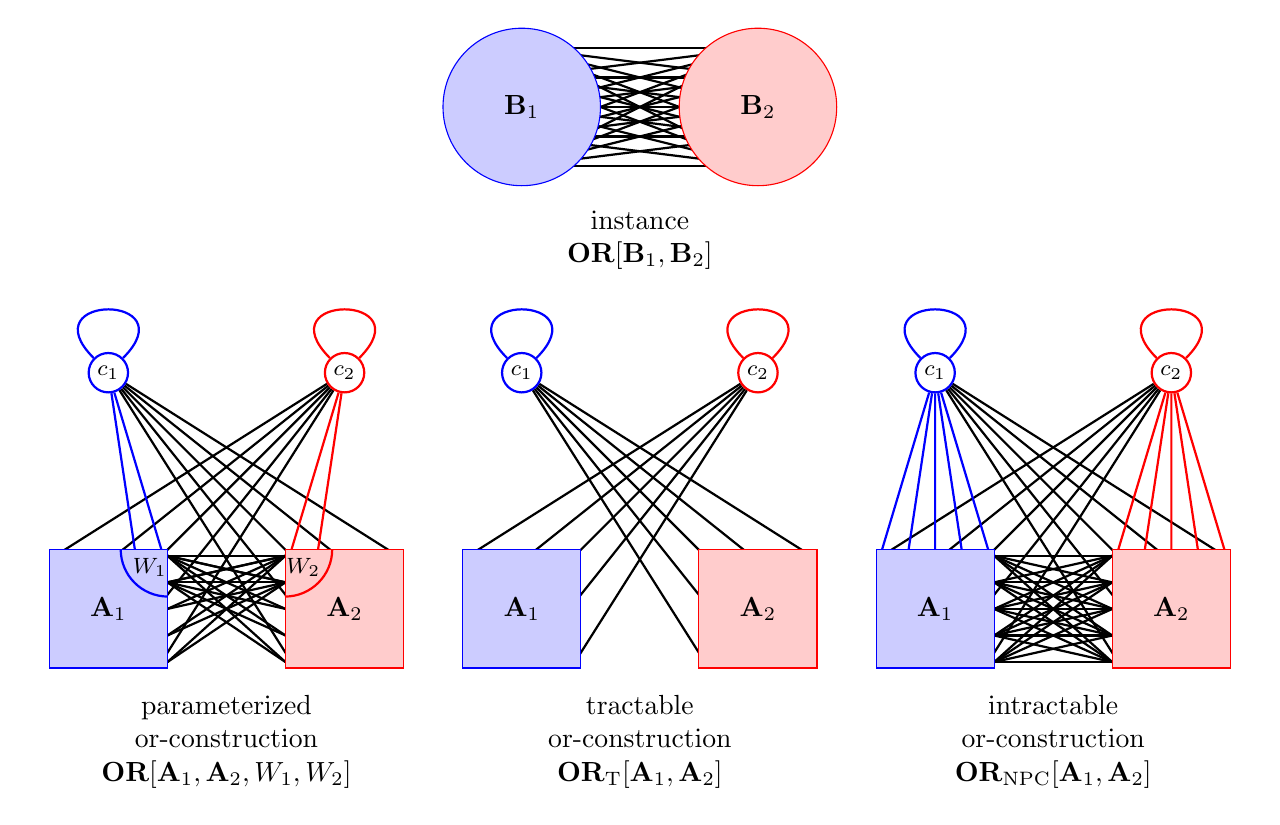
\begin{tikzpicture}[scale=0.75]
			\colorlet{col1}{blue}
			\colorlet{col2}{red}
			\colorlet{colInstance}{red}
			
			\tikzstyle{template1} = [draw=col1, fill=col1!20!white, text=black, rectangle, minimum width=1.5cm, minimum height=1.5cm];
			\tikzstyle{template2} = [draw=col2, fill=col2!20!white, text=black, rectangle, minimum width=1.5cm, minimum height=1.5cm];
			\tikzstyle{instance1} = [draw=col1, fill=col1!20!white, text=black,  circle, minimum width=2cm, minimum height=2cm];
			\tikzstyle{instance2} = [draw=col2, fill=col2!20!white, text=black,  circle, minimum width=2cm, minimum height=2cm];
			\tikzstyle{vertex} = [fill=none, minimum width =0.5cm, minimum height = 0.5cm, thick, circle, inner sep = 0mm, font=\footnotesize];
			
			\tikzstyle{sedge} = [black, thick];
			
			\begin{scope}[shift={(7.5,12.5)}]
				\node [instance1] (b1) at (-2,-2) {$\StructB_1$};
				\node [instance2] (b2) at (2,-2) {$\StructB_2$};
				
				
				\begin{scope}[on background layer]	
					
					\def\ystep{0.5}
					\foreach \i in {-2,...,2}{
						\foreach \j in {-2,...,2} {
							\draw[thick, sedge] ($(b1) + (0,\i*\ystep)$) --($(b2) + (0,\j*\ystep)$);
						}
					}
				\end{scope}
				
				\node[text width=3cm, align=center] at (0,-4.25) {instance\\$\OR{\StructB_1,\StructB_2}$};
				
			\end{scope}
			
			
			\def\adstep{0.45}
			\def\avstep{0.45}
			\def\wstep{0.25}
			
			\begin{scope}[shift = {(0.5,0)}]
				\node [template1, vertex] (c1) at (-2,6) {$c_1$};
				\node [template2, vertex] (c2) at (2,6) {$c_2$};
				\node [template1] (a1) at (-2,2) {$\StructA_1$};
				\node [template2] (a2) at (2,2) {$\StructA_2$};
				\draw [col1, thick] ($(a1.north east)-(0.8,0)$) arc (180:270:0.8cm);
				\draw [col2, thick] ($(a2.north west)-(0,0.8)$) arc (270:360:0.8cm);
				\node[font=\footnotesize] (w1) at (-1.3,2.7)  {$W_1$};
				\node[font=\footnotesize] (w2) at (1.3,2.7)  {$W_2$};
				
				
				
				
				\begin{scope}[on background layer, every loop/.style={}]
					
					\foreach \i in {-2,...,2}{
						\draw[thick, sedge] ($(a1.center) + (\i*\adstep,-\i*\adstep)$) --(c2);
						\draw[thick, sedge] ($(a2) + (\i*\adstep,\i*\adstep)$) --(c1);
					}
					
					
					
					\foreach \i in {-2,...,2}{
						\foreach \j in {1,...,2} {
							\draw[thick, sedge] ($(a2) + (-1,\i*\avstep)$) --($(a1) + (1,\j*\avstep)$);
							\draw[thick, sedge] ($(a1) + (1,\i*\avstep)$) --($(a2) + (-1,\j*\avstep)$);
						}
					}
					
					\foreach \i in {1,...,2}{
						\draw[thick, col1] ($(a1) + (\i*\avstep,1)$) --(c1);
						\draw[thick, col2] ($(a2) + (-\i*\avstep,1)$) --(c2);
					}
					
					\draw [thick, col1] (c1) edge [loop] (c1);
					\draw [thick, col2] (c2) edge [loop] (c2);
				\end{scope}
				
				\node[text width=3.5cm, align=center] at (0,-0.25) {parameterized or-construction\\$\ORparam{\StructA_1,\StructA_2,W_1,W_2$}};
			\end{scope}
			
			\begin{scope}[shift = {(7.5,0)}]
				\node [template1, vertex] (c1) at (-2,6) {$c_1$};
				\node [template2, vertex] (c2) at (2,6) {$c_2$};
				\node [template1] (a1) at (-2,2) {$\StructA_1$};
				\node [template2] (a2) at (2,2) {$\StructA_2$};
				
				
				\begin{scope}[on background layer, every loop/.style={}]
					
					\foreach \i in {-2,...,2}{
						\draw[thick, sedge] ($(a1.center) + (\i*\adstep,-\i*\adstep)$) --(c2);
						\draw[thick, sedge] ($(a2) + (\i*\adstep,\i*\adstep)$) --(c1);
					}
					
					
					\draw [thick, col1] (c1) edge [loop] (c1);
					\draw [thick, col2] (c2) edge [loop] (c2);
				\end{scope}
				
				\node[text width=3cm, align=center] at (0,-0.25) {tractable\\ or-construction\\$\ORT{\StructA_1,\StructA_2}$};
			\end{scope}
			
			\begin{scope}[shift = {(14.5,0)}]
				\node [template1, vertex] (c1) at (-2,6) {$c_1$};
				\node [template2, vertex] (c2) at (2,6) {$c_2$};
				\node [template1] (a1) at (-2,2) {$\StructA_1$};
				\node [template2] (a2) at (2,2) {$\StructA_2$};
				
				
				\begin{scope}[on background layer, every loop/.style={}]
					
					\foreach \i in {-2,...,2}{
						\draw[thick, sedge] ($(a1.center) + (\i*\adstep,-\i*\adstep)$) --(c2);
						\draw[thick, sedge] ($(a2) + (\i*\adstep,\i*\adstep)$) --(c1);
					}
					
					
					\foreach \i in {-2,...,2}{
						\foreach \j in {-2,...,2} {
							\draw[thick, sedge] ($(a2) + (-1,\i*\avstep)$) --($(a1) + (1,\j*\avstep)$);
						}
					}
					
					\foreach \i in {-2,...,2}{
						\draw[thick, col1] ($(a1) + (\i*\avstep,1)$) --(c1);
						\draw[thick, col2] ($(a2) + (\i*\avstep,1)$) --(c2);
					}
					
					\draw [thick, col1] (c1) edge [loop] (c1);
					\draw [thick, col2] (c2) edge [loop] (c2);
				\end{scope}
				\node[text width=3cm, align=center] at (0,-0.25) {intractable or-construction\\$\ORNPC{\StructA_1,\StructA_2}$};
			\end{scope}
		\end{tikzpicture}
		\caption{The different homomorphism or-constructions:
			The picture assumes that the two vocabularies $\sig_1$ and $\sig_2$
			are binary and contain a single relation each (blue and red).
			At the top the instance $\OR{\StructB_1,\StructB_2}$.
			At the bottom three different version on the templates:
			the general parameterized construction,
			and the special cases of the tractable and intractable construction,
			which will be discussed in Sections~\ref{app:tractable-or} and~\ref{app:intractable-or}, respectively.
			The new $S$-relation is drawn in black,
			where the edges are all oriented from left to right.
			Pairs added to the relation of $\sig_1$ or $\sig_2$
			are drawn in blue or red, respectively.
			\label{fig:hom-or-construction}
		}
	\end{figure}	
	\noindent Figure~\ref{fig:hom-or-construction} illustrates the construction.
	The following lemma shows that this definition yields a homomorphism or-construction independently of the sets $W_i$.
	As we will see, the choice of $W_i$ controls embeddings of partial homomorphisms 
	and the complexity of the resulting template.
	We will later work with two concrete instantiations of the sets $W_i$, one of which yields a tractable and the other an intractable or-construction. But first we prove all properties that hold for any choice of $W_i$.
	
	\begin{lemma}
		\label{lem:hom-or-construction-correct}
		$\StructB \in \CSP{\StructA}$ if and only if there is an $i \in [2]$
		such that $\StructB_i \in \CSP{\StructA_i}$.
	\end{lemma}
	\begin{proof}\textcolor{red}{TOPROVE 4}\end{proof}
	
	\noindent We now analyze which partial homomorphisms $\StructB_i \to \StructA_i$
	can be extended to partial or global homomorphisms $\StructB \to \StructA$.
	For $i\in[2]$, denote by $\restrict{\StructA}{i}$ the structure $\StructA[A_i\cup\set{c_i}]$.
	
	\begin{lemma}
		\label{lem:hom-or-embedd}
		Let $i \in [2]$, $X \subseteq B_i$, and
		$f \in \Hom{\StructB_i[X]}{\StructA_i}$.
		Then $f \in \Hom{\StructB[X]}{\restrict{\StructA}{i}}$.
	\end{lemma}
	\begin{proof}\textcolor{red}{TOPROVE 5}\end{proof}
	
	\begin{lemma}
		\label{lem:hom-or-extend}
		Let $i \in [2]$.
		For every $X \subseteq B_i$ and $f\in \Hom{\StructB_i[X]}{\restrict{\StructA}{i}[(W_i\cup \set{c_i})]}$,
		the map $g \colon B_i \to W_i \cup \set{c_i}$ defined by
		\begin{align*}
			g(b) := \begin{cases}
				f(b) & \text{if } b \in X, \\
				c_i	& \text{otherwise.}
			\end{cases}
		\end{align*}
		is a homomorphism in  $\Hom{\StructB[B_i]}{\restrict{\StructA}{i}[W_i\cup \set{c_i}]}$.
		It satisfies in particular $\restrict{g}{X} = f$. 
	\end{lemma}
	\begin{proof}\textcolor{red}{TOPROVE 6}\end{proof}
	
	\begin{lemma}
		\label{lem:hom-or-compose}
		Let $X_i \subseteq B_i$ and $f_i \in \Hom{\StructB[X_i]}{\restrict{\StructA}{i}}$ for both $i\in[2]$.
		Let $f\colon X_1\cup X_2 \to A$ be the map defined by each $f_i$ on $X_i$ for $i \in[2]$.
		If there is an $i\in[2]$ such that $c_i \notin f_i(X_i)$
		and $f_{3-i}(B_{3-i}) \subseteq W_{3-i} \cup \set{c_{3-i}}$,
		then $f \in \Hom{\StructB[X_1\cup X_2]}{\StructA}$.
	\end{lemma}
	\begin{proof}\textcolor{red}{TOPROVE 7}\end{proof}
	
	\begin{corollary}
		\label{cor:hom-or-compose-simple}
		Let $i \in [2]$ and $f_i \in \Hom{\StructB_i}{\StructA_i}$.
		Assume $X \subseteq B_{3-i}$ and let 
		$f_{3-i} \in \Hom{\StructB_{3-i}[X]}{\StructA_{3-i}[W_{3-i}]}$.
		Then there is a $g \in \Hom{\StructB}{\StructA}$
		that agrees with $f_i$ on $B_i$ and with $f_{3-i}$ on $X$.
	\end{corollary}
	\begin{proof}\textcolor{red}{TOPROVE 8}\end{proof}
	
	\noindent Next, we show that the homomorphism or-construction is compatible
	with $k$-consistency and solving $\cspiso{k}{\StructA}{\StructB}$
	in the sense that if $k$-consistency
	accepts $\StructB_i$, or $\cspiso{k}{\StructA_i}{\StructB_i}$
	is satisfiable,
	then $k$-consistency accepts $\StructB$, or $\cspiso{k}{\StructA}{\StructB}$
	is satisfiable, respectively.
	
	\begin{lemma}
		\label{lem:hom-or-k-consistency}
		Let $k \in \nat$, $X_i \subseteq B_i$  and $f_i \in \Hom{\StructB[X_i]}{\restrict{\StructA}{i}}$ for both $i\in[2]$
		such that $|X_1 \cup X_2|\leq k$.
		Let $f \colon X_1\cup X_2 \to A$ be the map induced by $f_1$ and $f_2$.
		If there is an $i\in[2]$ such that  
		\begin{itemize}
			\item $f_i \in \kcol{k}{\StructA_i}{\StructB_i}(X_i)$
			(so in particular $c_i \notin f_i(X_i)$),
			\item $f_{3-i}(X_{3-i}) \subseteq W_{3-i} \cup \set{c_{3-i}}$, and
			\item for $X_{3-i}' := \inv{f_{3-i}}(W_{3-i})$ we have $\restrict{f_{3-i}}{X_{3-i}'} \in \kcol{k}{\StructA_{3-i}}{\StructB_{3-i}}(X_{3-i}')$,
		\end{itemize}
		then $f \in \kcol{k}{\StructA}{\StructB}(X_1 \cup X_2)$.
	\end{lemma}
	\begin{proof}\textcolor{red}{TOPROVE 9}\end{proof}
	
	\begin{lemma}
		\label{lem:hom-or-solution}
		Let  $i \in [2]$ and assume that $\Phi$ is a solution to $\cspiso{k}{\StructA_i}{\StructB_i}$.
		Furthermore, let $h \in \Hom{\StructB_{3-i}}{\restrict{\StructA}{3-i}[W_{3-i}\cup\set{c_{3-i}}]}$.
		Then the following map $\Psi$ is a solution to $\cspiso{k}{\StructA}{\StructB}$.
		Let $X \in \tbinom{\StructB}{\leq k}$, $X_j := X \cap B_j$ for $j\in[2]$, and $f \in \Hom{\StructB[X]}{\StructA}$.
		We set
		\[
		\Psi(x_{X,f}) := \begin{cases}
			\Phi(x_{X_i, \restrict{f}{X_i}}) & \text{if }
			\restrict{f}{X_i} \in \Hom{\StructB_i[X_i]}{\StructA_i} \text { and } \restrict{f}{X_{3-i}} = \restrict{h}{X_{3-i}}\\
			0 & \text{otherwise.}
		\end{cases}
		\]
		In particular, if $\Phi$ is an integral solution or a $p$-solution,
		then $\Psi$ is an integral solution or $p$-solution, respectively.
	\end{lemma}
	\begin{proof}\textcolor{red}{TOPROVE 10}\end{proof}
	
	
	
	
	
	
	\subsection{The Tractable Case}
	\label{app:tractable-or}
	We now consider the case that $W_1=W_2=\emptyset$.
	In this setting, the homomorphism or-construction yields a tractable CSP
	if $\CSP{\StructA_i}$ is tractable for both $i\in[2]$.
	We refer to this construction as the \defining{tractable homomorphism or-construction} and write $\ORT{\StructA_1,\StructA_2} := \ORparam{\StructA_1,\StructA_2,\emptyset,\emptyset}$.
	We start with corollaries from the lemmas of the previous subsection:
	
	
	\homOrTractableKConsistency*
	\begin{proof}\textcolor{red}{TOPROVE 11}\end{proof}
	
	\homOrTractableSolution*
	\begin{proof}\textcolor{red}{TOPROVE 12}\end{proof}
	
	\noindent We now prove that the tractable or-construction indeed deserves its name because it generally preserves tractability of $\StructA_1$ and $\StructA_2$. In the special case of Maltsev templates, also this stronger condition is preserved: 
	
	\maltsevForOrConstruction*
	\begin{proof}\textcolor{red}{TOPROVE 13}\end{proof}	
	
	\noindent In particular, the above lemma shows tractability of the or-construction in the case that $\CSP{\StructA_1}$ and $\CSP{\StructA_2}$ have a Maltsev polymorphism.
	The next lemma shows this for the general case that $\CSP{\StructA_1}$ and $\CSP{\StructA_2}$ are tractable by providing a polynomial-time algorithm
	for $\CSP{\ORT{\StructA_1,\StructA_2}}$.
	More strongly, we will show, using that algorithm, that if both $\CSP{\StructA_i}$
	are definable in a logic subsuming inflationary fixed-point logic,
	then so is $\CSP{\ORT{\StructA_1,\StructA_2}}$.
	
	\homOrTractable*
	\begin{proof}\textcolor{red}{TOPROVE 14}\end{proof}
	
	\homOrDefinable*
	\begin{proof}\textcolor{red}{TOPROVE 15}\end{proof}
	
	\noindent We will use the tractable homomorphism or-construction to build
	tractable CSPs that are not solved correctly by the algorithms in Theorem \ref{thm:mainResultInformal}.
	We consider templates $\StructA_1$ and $\StructA_2$ for which the tractable or-construction $\StructA = \ORT{\StructA_1,\StructA_2}$ will guarantee the existence of integral solutions to $\cspiso{\StructA}{k}{\StructB}$ for certain instances $\StructB = \OR{\StructB_1,\StructB_2} \notin \CSP{\StructA}$. This will in particular be the case even though no such integral solution exists for $\cspiso{\StructA_1}{k}{\StructB_1}$ and $\cspiso{\StructA_2}{k}{\StructB_2}$.
	However, the \emph{cohomological $k$-consistency} algorithm will be able to tell that $\cspiso{\StructA_1}{k}{\StructB_1}$ and $\cspiso{\StructA_2}{k}{\StructB_2}$ do not have an integral solution, and this will be sufficient for it to correctly output that $\StructB \notin \CSP{\StructA}$. The next two lemmas are the technical foundation for this and will be used in the proof of the first part of Theorem \ref{thm:mainPowerOfCohomology}.
	The crucial point is that the cohomological algorithm considers solutions to $\cspiso{\StructA}{k}{\StructB}$ in which for certain sets $X$, every $f: X \to A$ that has $c_i$ in its image receives value $0$.
	
	\begin{lemma}
		\label{lem:fixingIntegerSolutionInOr}
		Let $k \geq 2$, $i \in [2]$, 
		and $\Phi$ be a solution to $\cspiso{\StructA}{k+1}{\StructB}$.
		If there is a set $Z \in \tbinom{B_i}{\leq k}$ such that
		for every $f\in \Hom{\StructB[Z]}{\StructA}$ with $c_i \in f(Z)$
		it holds that
		$\Phi(x_{Z,f}) = 0$, then we have $\Phi(x_{X,g}) = 0$
		for every $X \in \tbinom{B_i}{\leq k}$ and every
		$g\in \Hom{\StructB[X]}{\StructA}$ with $c_i \in f(X)$.
	\end{lemma}
	\begin{proof}\textcolor{red}{TOPROVE 16}\end{proof}
	
	\integerSolutionWithLocalFixingSolvesBi*
	\begin{proof}\textcolor{red}{TOPROVE 17}\end{proof}
	
	\noindent From this lemma it follows that the tractable homomorphism or-construction 
	cannot be used to make CSPs harder for algorithms that solve $\cspiso{k}{\StructA}{\StructB}$ over the integers
	and fix local solutions.
	To deal with this and be able to prove the second part of Theorem \ref{thm:mainPowerOfCohomology}, we now sacrifice tractability of the homomorphism or-construction, which will also make it harder for the cohomological algorithm.
	
	
	
	\subsection{The Intractable Case}
	\label{app:intractable-or}
	This section deals with the case that $W_1 =A_1$ and $W_2 = A_2$.
	In this case, the homomorphism or-construction has the drawback to yield an NP-complete CSP even if $\CSP{\StructA_1}$ and $\CSP{\StructA_2}$ are tractable.
	But it has the benefit that more partial homomorphisms can be extended to global ones, in particular if $\StructB_1\in\CSP{\StructA_1}$ and $\StructB_2 \notin \CSP{\StructA_2}$,
	we can still extend partial homomorphisms $\StructB_2 \to \StructA_2$ to
	global homomorphisms.
	We set $\ORNPC{\StructA_1,\StructA_2} := \ORparam{\StructA_1,\StructA_2,A_1,A_2}$.
	We refer to this as the \defining{intractable homomorphism or-construction}.
	We again start with corollaries from the general or-construction.
	
	\homOrIntractableCompose*
	\begin{proof}\textcolor{red}{TOPROVE 18}\end{proof}
	
	\begin{lemma}
		\label{lem:hom-or-intractable-k-consistency}
		Assume $\StructA=\ORNPC{\StructA_1,\StructA_2}$
		and $\StructB = \OR{\StructB_1,\StructB_2}$.
		Let $k \in \nat$, $X_i \subseteq B_i$  and $f_i \in \Hom{\StructB_i}{\StructA_i}$ for both $i\in[2]$
		such that $|X_1 \cup X_2|\leq k$.
		If for some $i\in [2]$
		we have $f_i \in \kcol{k}{\StructA_i}{\StructB_i}(X_i)$,
		then the map $f\colon X_i\cup X_2 \to A$ induced by $f_1$ and $f_2$
		satisfies $f \in \kcol{k}{\StructA}{\StructB}(X_1 \cup X_2)$.
	\end{lemma}
	\begin{proof}\textcolor{red}{TOPROVE 19}\end{proof}
	
	\begin{lemma}
		\label{lem:hom-or-intractable-solution}
		Assume $\StructA=\ORNPC{\StructA_1,\StructA_2}$
		and $\StructB = \OR{\StructB_1,\StructB_2}$.
		Let  $i \in [2]$, let $\Phi$ be a solution to $\cspiso{k}{\StructA_i}{\StructB_i}$,
		and let $Y \subseteq B_{3-i}$ and $h \in \Hom{\StructB_{3-i}[Y]}{\StructA_{3-i}}$.
		Then there is a solution~$\Psi$ to $\cspiso{k}{\StructA}{\StructB}$
		such that for every $X \in \tbinom{\StructB}{\leq k}$ and $f \in \Hom{\StructB[X]}{\StructA}$,
		$\Psi(x_{X,f})\neq 0$ implies
		$\Psi(x_{X,f}) = \Phi(x_{X\cap B_i, \restrict{f}{X\cap B_i}})$
		and $\restrict{f}{X\cap Y} = \restrict{h}{X\cap Y}$.
		In particular, if $\Psi(x_{Y,h}) = 1$
		and $\Phi$ is an integral solution or a $p$-solution,
		then $\Psi$ is an integral solution or $p$-solution, respectively.
	\end{lemma}
	\begin{proof}\textcolor{red}{TOPROVE 20}\end{proof}
	
	
	The following lemmas show that the intractable homomorphism or-construction yields an NP-complete CSP if for both $\StructA_i$ there are non-trivial
	no-instances for $\CSP{\StructA_i}$.
	We start to consider the very simple case  that both $\StructA_i$ are of size $1$
	and contain a ternary relation that is empty.
	For a ternary relational symbol $R$,
	denote by $\onestruc{R}$ such a $\set{R}$-structure.
	
	\begin{lemma}
		\label{lem:intractable-or-NPC-basic}
		Let $R_i$ be ternary relation symbols and
		$\StructA_i := \onestruc{R_i}$.
		Then $\CSP{\ORNPC{\StructA_1,\StructA_2}}$ is NP-complete.
	\end{lemma}
	\begin{proof}\textcolor{red}{TOPROVE 21}\end{proof}
	
	The next lemma shows that many CSPs reduce to the one in the following lemma.
	We call a no-instance of a CSP \defining{inclusion-wise minimal}
	if every proper induced subinstance of it is a yes-instance.
	The following lemma requires that each $\StructA_i$
	has a inclusion-wise minimal no-instance of order at least $3$.
	This covers many CSPs, for example many kinds of equation systems,
	group coset CSPs, but also $\CSP{P_1}$ with $K_3$ as inclusion-wise minimal no instance (where $P_1$ is the path of length one and $K_3$ the triangle).
	
	\begin{lemma}
		\label{lem:intractable-or-NPC-reduce}
		Let $R_i$ be ternary relation symbols
		and $\StructA_i$ be $\sig_i$-structures for $i\in[2]$.
		If for both $i \in [2]$,
		there is a inclusion-wise minimal $\sig_i$-structure $\StructC_i \notin \CSP{\StructA_i}$
		of order at  least $3$,
		then $\ORNPC{\onestruc{R_1}, \onestruc{R_2}}$ is Karp-reducible to $\ORNPC{\StructA_1,\StructA_2}$.
	\end{lemma}
	\begin{proof}\textcolor{red}{TOPROVE 22}\end{proof}
	
	
	\section{Details on the Tseitin-Systems}
	\label{app:tseitin}
	
	In the following, we assume the set-up from Section \ref{sec:tseitin}. The value $k \in \bbN$ is thought of as a constant, but
	unless explicitly stated otherwise, the following lemmas also hold in case that $k$ is a function in $|E|$ that grows at most sublinearly. 
	\begin{lemma}
		\label{lem:robustly-consistent-for-all-small-contexts}
		For all $\lambda \colon V\to \Gamma$ and $X \in \tbinom{E}{\leq k}$,
		there is a robustly consistent partial assignment $f \colon X \to \Gamma$ for $\grpCSPf{H}{\Gamma}{\lambda}$. 
	\end{lemma}
	\begin{proof}\textcolor{red}{TOPROVE 23}\end{proof}	
	


	\noindent When we view $\grpCSPf{H}{\Gamma}{\lambda}$ as a homomorphism problem,
	then for every $X \subseteq E$,
	a partial solution $f \colon X \to \Gamma$ of $\grpCSPf{H}{\Gamma}{\lambda}$ (so in particular a robustly consistent partial assignment)
	is a homomorphism in $\Hom{\grpCSPf{H}{\Gamma}{\lambda}}{\CosetGrpTmplt{\Gamma}{3}}$
	and vice versa
	(recall that $\CosetGrpTmplt{\Gamma}{3}$ is the template structure for $3$-ary $\Gamma$-coset-CSPs).
	
	\begin{lemma}
		\label{lem:robustlyConsistentSurviveKconsistency}
		For every $\lambda \colon V \to \Gamma$,
		the $k$-consistency algorithm does not rule out any robustly consistent partial assignments.
		This means that, for every $X \in \binom{E}{\leq k}$,  every robustly consistent assignment
		contained in $\Hom{\grpCSPf{H}{\Gamma}{\lambda}[X]}{\CosetGrpTmplt{\Gamma}{3}}$
		is contained in $\kcol{k}{\CosetGrpTmplt{\Gamma}{3}}{\grpCSPf{H}{\Gamma}{\lambda}} (X)$.
	\end{lemma}
	\begin{proof}\textcolor{red}{TOPROVE 24}\end{proof}
	
	
	\begin{corollary}
		\label{cor:kConsistencyFails}
		For all $\lambda \colon V \to \Gamma$ and $X \in \binom{E}{\leq k}$,
		we have $\kcol{k}{\CosetGrpTmplt{\Gamma}{3}}{\grpCSPf{H}{\Gamma}{\lambda}}(X) \neq \emptyset$.
	\end{corollary}	
	\begin{proof}\textcolor{red}{TOPROVE 25}\end{proof}	
	
	
	
	\noindent For a prime $p$, a \defining{$p$-group} is a group in which the order of every element is a power of $p$. For instance, $\bbZ_2$ is a $2$-group and $\bbZ_3$ a $3$-group.
	
	
	
	
	\noindent We now need to consider the case when one robustly consistent partial solution $f: Z \to \Gamma$, with $Z \in \binom{E(G)}{\leq k}$ is fixed.
	We show that in this case
	the system $\cspiso{k}{\CosetGrpTmplt{\Gamma}{3}}{\grpCSPf{H}{\Gamma}{\lambda}}$ has a solution in which $x_{Z,f}$ is set to $1$.
	Fix a set $\hat{Z} \supseteq Z$ such that $E(G) \setminus \hat{Z}$ is the edge set of a $2$-connected subgraph of $G$.
	By the expansion property, we can choose it such that $|\hat{Z}| \leq c \cdot |Z|$, where $c$ is the expansion constant. 
	\begin{lemma}
		\label{lem:fHatCanBeExtended}
		There is an assignment $h : \hat{Z} \to \Gamma$ such that $h|_{Z} = f$, and $h \in \Hom{\grpCSPf{H}{\Gamma}{\lambda}[\hat{Z}]}{\CosetGrpTmplt{\Gamma}{3}}$ is robustly consistent.
	\end{lemma}	
	\begin{proof}\textcolor{red}{TOPROVE 26}\end{proof}	
	\noindent Fix this partial solution $h \colon \hat{Z} \to \Gamma$ 
	for $\grpCSPf{H}{\Gamma}{\lambda}$ given by Lemma~\ref{lem:fHatCanBeExtended} in the following.
	Let $G'=(V',E')$ be the graph obtained from $G$ by deleting all edges in $\hat{Z}$
	and all vertices that are not in the $2$\nobreakdash-connected component of $G-\hat{Z}$.
	Similarly, obtain the directed graph $H'$ from $H$ by deleting the same (directed) edges and vertices.
	Let $\lambda' : V' \to \Gamma$ be defined as follows. For every $v \in V'$, set
	\[
	\lambda'(v) := \lambda(v) - \sum_{e \in \delta_+(v) \cap \hat{Z}} h(y_e) + \sum_{e \in \delta_-(v) \cap \hat{Z}} h(y_e) .
	\] 
	With this definition, $\grpCSP{H'}{\Gamma}{\lambda'}$ is the CSP that we obtain from $\grpCSPf{H}{\Gamma}{\lambda}$ by fixing values for the variables in~$\hat{Z}$ according to $h$ from Lemma \ref{lem:fHatCanBeExtended}. In what follows, let $\StructC = \grpCSP{H}{\Gamma}{\lambda}$
	and $\StructC' = \grpCSP{H'}{\Gamma}{\lambda'}$.
	The graph~$G'$ is still an expander:
	\begin{lemma}
		\label{lem:expandersRobust}
		Let $k \in \bbN$ and $(G_n)_{n \in \bbN}$ a family of expander graphs with expansion constant $c$. Fix a set $X_n \in \binom{E(G_n)}{\leq k}$ for every $n$.
		Let $G'_n$ be the $2$-connected subgraph of $G_n$ that remains after removing the edges $\hat{X}_n \supseteq X_n$ (and potentially isolated vertices) from $G_n$. Then $(G'_n)_{n \in \bbN}$ is also a family of expander graphs (with a different expansion constant that depends on $k$ and $c$).
	\end{lemma}	
	\begin{proof}\textcolor{red}{TOPROVE 27}\end{proof}	
	
	
	
	
	\begin{lemma}
		\label{lem:piecingTogetherPhiAndSolution}
		If $\cspiso{k}{\CosetGrpTmplt{\Gamma}{3}}{\StructC'}$ has a $p$-solution $\Phi$, then $\cspiso{k}{\CosetGrpTmplt{\Gamma}{3}}{\StructC}$ has a $p$-solution $\Psi$ such that
		\begin{enumerate}
			\item if $\Phi(x_{X',f'}) = 0$, then $\Psi(x_{X,f}) = 0$, for every $X$ with $X \cap E' = X'$ and $f|_{E'} = f'$.
			\item  for all sets of variables $X \in \binom{E \setminus E'}{\leq k}$ of the system $\StructC$ and for all partial homomorphisms $f \in \Hom{\StructC[X]}{\CosetGrpTmplt{\Gamma}{3}}$,
			we have $\Psi(x_{X,f}) = 1$ if $f$ agrees with $h$, and $\Psi(x_{X,f}) = 0$, otherwise.
		\end{enumerate}
	\end{lemma}	
	\begin{proof}\textcolor{red}{TOPROVE 28}\end{proof}	
	
	
	
	\begin{corollary}
		\label{cor:group-csp-p-solution-with-fixed-assignment}
		Let $k \in \bbN$ be a constant and explicitly not a function of $|E|$.
		Let $Z \in \binom{E(G)}{\leq k}$ and assume that $\Gamma$ is a $p$-group.
		If $f \in \Hom{\StructC[Z]}{\Gamma}$ is robustly consistent, then $\cspiso{k}{\Gamma}{\StructC}$ has a $p$-solution $\Psi$ such that
		\begin{itemize}
			\item $\Psi$ is $0$ for partial assignments that are not robustly consistent.
			\item $\Psi(x_{Z,f}) = 1$.
		\end{itemize}
	\end{corollary}
	\begin{proof}\textcolor{red}{TOPROVE 29}\end{proof}	
	
	
	
	
	
	
	
	
	\section{Details on the Limitations of the Affine Algorithms}
	\label{app:power-of-affine}
	
	This section introduces the algorithms from Theorem \ref{thm:mainResultInformal}
	and shows that each of them fails to solve the same CSP:
	the tractable homomorphism or-construction
	of ternary $\ZZ_2$-coset-CSP and  ternary $\ZZ_3$-coset-CSP
	$\ORT{\CosetGrpTmplt{\ZZ_2}{3}, \CosetGrpTmplt{\ZZ_3}{3}}$.
	
	
	\subsection{\texorpdfstring{$\ZZ$}{ℤ}-Affine \texorpdfstring{$k$}{k}-Consistency Relaxation}
	\label{app:zAffineConsistency}
	
	
	We first consider the \defining{$\ZZ$-affine $k$-consistency relaxation},
	an algorithm proposed by Dalmau and Opr\v{s}al~\cite{DalmauOprsal2024}.
	The algorithm considers the following system of affine linear equations over the integers.
	Let $\StructA$ be a template structure, $\StructB$ be an instance,
	and $\kappa$ be a map
	that assigns to every set  $X \in \binom{B}{\leq k}$ a set of partial homomorphisms $\StructB[X] \to \StructA$.
	The system $\zafkleq{k}{\StructA}{\StructB}{\kappa}$
	is defined as follows: 
	
	\begin{systembox}{$\zafkleq{k}{\StructA}{\StructB}{\kappa}$: variables $z_{X,f}$
			for all $X \in {\tbinom{B} {\leq k}}$
			and $f \in \kappa(X)$}
		\begin{align*}
			z_{X,f} &\in \ZZ &  \text{for all } X \in \tbinom{B}{\leq k} \text { and } f \in \kappa(X)\tag{Z1}\\
			\sum_{f \in \kappa(X)}  z_{X,f}&= 1 &  \text{for all } X \in \tbinom{B}{\leq k}\label{eqn:zaff-sum-to-one}\tag{Z2}\\
			\sum_{f \in \kappa(X), \restrict{f}{Y} = g} z_{X,f} &= z_{Y,g} & \text{for all } Y\subset X \in \tbinom{B}{\leq k} \text { and } g \in \kappa(Y) \label{eqn:zaff-agree}\tag{Z3}
		\end{align*}
	\end{systembox}
	
	\noindent Recall that $\kcol{k}{\StructA}{\StructB}$ denotes the output of the $k$-consistency algorithm,
	which is a function that  assigns partial homomorphisms to each set $X \in \binom{B}{\leq k}$.
	The $\ZZ$-affine $k$-consistency relaxation runs, for a fixed positive integer $k$ and a template structure $\StructA$, as follows:
	\begin{algobox}{$\ZZ$-affine $k$-consistency relaxation for template $\StructA$: input a $\CSP{\StructA}$-instance $\StructB$}
		\begin{enumerate}
			\item Compute $\kcol{k}{\StructA}{\StructB}$ using the $k$-consistency algorithm.
			\item Accept if the system $\zafkleq{k}{\StructA}{\StructB}{\kcol{k}{\StructA}{\StructB}}$ is solvable and reject otherwise.
		\end{enumerate}
	\end{algobox}
	
	
	\noindent Dalmau and Opr\v{s}al~\cite{DalmauOprsal2024} made the following
	conjecture on the power of the $\ZZ$-affine $k$-consistency relaxation:
	\sthreeorZ*
	\noindent The latter case of the conjecture considers a reduction to systems of linear equation systems over the integers.
	This condition in particular implies
	that $\CSP{\StructA}$ is solved by the  $\ZZ$-affine $k$-consistency algorithm for some constant $k$~\cite{DalmauOprsal2024}.
	
	
	
	
	\zAffineDoesNotSolveBoundedColorClass*
	\begin{proof}\textcolor{red}{TOPROVE 30}\end{proof}
	
	\notDatalogReducible*
	\begin{proof}\textcolor{red}{TOPROVE 31}\end{proof}
	
	\noindent
	Theorem~\ref{thm:z-affine-does-not-solve-bounded-color-class}
	and Lemma~\ref{lem:not-datalog-reducible}
	disprove Conjecture~\ref{con:s3-or-Z}.
	
	\subsection{BLP+AIP and BA\texorpdfstring{$^k$}{k}}
	\label{app:BLP}
	Before considering the next algorithm,
	we first introduce a well-studied system of equations for CSPs~\cite{BartoBKO2021,BrakensiekGWZ2020}, or, more precisely, 
	a variant of it parameterized by the size of partial solutions~\cite{CiardoZivny2023GraphColoring}.
	Let $k$ be a positive integer, $\StructA$ a template $\sig$-structure
	and~$\StructB$ a $\CSP{\StructA}$-instance.
	We define the system
	$\ipk{k}{\StructA}{\StructB}$ with variable set $\VarsIP{k}{\StructA}{\StructB}$.
	\begin{systembox}{$\ipk{k}{\StructA}{\StructB}$: 
			variables $\lambda_{X,f}$ for all $X \in \tbinom{B}{\leq k}$ and  $f\colon X \to A$, and \\\phantom{$\ipk{k}{\StructA}{\StructB}$: }variables $\mu_{R,\tup{b},\tup{a}}$ for all $R \in \sig$, $\tup{b} \in R^\StructB$, and $\tup{a} \in R^\StructA$}
		\begin{align}
			\sum_{f \colon X \to A} \lambda_{X,f} &= 1  &\text{for all } X \in \tbinom{B}{\leq k} \label{eqn:ip-only-one-local-solution}\tag{B1},\\
			\sum_{\substack{f \colon X \to A,\\\restrict{f}{Y} = g}} \lambda_{X,f} &= \lambda_{Y,g} & \text{for all } Y\subset X \in \tbinom{B}{\leq k}, g\colon Y \to A\label{eqn:local-solutions-consistent}\tag{B2},\\
			\sum_{\tup{a} \in R^\StructA, a_{\tup{i}} = \tup{a}'} \mu_{R,\tup{b},\tup{a}} &= \lambda_{X(\tup{b}_{\tup{i}}), \tup{b}_{\tup{i}} \mapsto \tup{a}' } &  \text {for all } R \in \sig, \tup{a}' \in A^k, \tup{b} \in R^\StructB, \tup{i} \in [\arity{R}]^k,\label{eqn:ip-hom}\tag{B3}
		\end{align}\\
		where $a_{\tup{i}}$ and $b_{\tup{i}}$ denote the $k$-tuples $(a_{\tup{i}_1},...,a_{\tup{i}_k})$ and $(b_{\tup{i}_1},...,b_{\tup{i}_k})$, respectively, $X(\tup{b}_{\tup{i}})$ denotes the set of entries of $\tup{b}_{\tup{i}}$, and $\tup{b}_{\tup{i}} \mapsto \tup{a}'$ denotes the partial homomorphism sending $\tup{b}_{\tup{i}}$ to $\tup{a}'$.
	\end{systembox}
	\noindent We consider different domains of the variables (see~\cite{BrakensiekGWZ2020}):
	\begin{itemize}
		\item If we restrict the variables to $\set{0,1}$, then
		$\ipk{1}{\StructA}{\StructB}$ is solvable if and only if
		$\StructB \in \CSP{\StructA}$.
		\item The relaxation of $\ipk{k}{\StructA}{\StructB}$ to nonnegative rationals is the \defining{basic linear programming (BLP)} relaxation $\blk{k}{\StructA}{\StructB}$.
		\item The affine relaxation of $\ipk{k}{\StructA}{\StructB}$ to all integers is the \defining{affine integer programming (AIP)} relaxation $\aipk{k}{\StructA}{\StructB}$.
	\end{itemize}
	By increasing the parameter~$k$, 
	the BLP and AIP relaxations result in the Sherali-Adams LP hierarchy and
	the affine integer programming hierarchy of the $\{0,1\}$-system, respectively.
	
	Brakensiek, Guruswami, Wrochna, and Živný \cite{BrakensiekGWZ2020} use a certain combination of $\blk{1}{\StructA}{\StructB}$ and $\aipk{1}{\StructA}{\StructB}$
	to formulate the \defining{BLP+AIP algorithm}.
	Similar to the $\ZZ$-affine $k$-consistency relaxation,
	the BLP+AIP algorithm tries to solve $\CSP{\StructA}$
	in the sense that it is sound.
	However, it may wrongly answer $\StructB \in \CSP{\StructA}$.
	The question is whether the BLP+AIP algorithm is also complete for tractable CSPs.
	In contrast to the $\ZZ$-affine $k$-consistency relaxation,
	the BLP+AIP algorithm is not parameterized by the size of partial solutions $k$.
	This parameterized version was proposed by Ciardo and Živný~\cite{CiardoZivny2023Tensors, CiardoZivny2023BAk}
	and is called \defining{BA$^k$}, where BA$^1$ is just the BLP+AIP algorithm.
	
	We now formally introduce this parameterized algorithm.
	Let $k$ be a positive integer.
	
	\begin{algobox}{$\BAk{k}{\StructA}$-algorithm: input a $\CSP{\StructA}$-instance $\StructB$}
		\begin{enumerate}
			\item Compute a relative interior point $\Phi \colon \VarsIP{k}{\StructA}{\StructB} \to \QQ $ in the polytope defined by $\blk{k}{\StructA}{\StructB}$.
			The solution $\Phi$ has in particular the property that for each variable $x \in \VarsIP{k}{\StructA}{\StructB}$ there is a solution $\Psi$ to $\blp{\StructA}{\StructB}$ such that $\Psi(x) \neq 0$
			if and only if $\Phi(x) \neq 0$.
			If such a point does not exist, reject.\label{itm:bak-interior-point}
			\item \label{item:bak-refined-constr} Refine $\aipk{k}{\StructA}{\StructB}$ by adding the constraints
			\[x = 0 \quad \text { whenever } \quad \Phi(x) = 0 \qquad \text{ for all }{x\in \VarsIP{k}{\StructA}{\StructB}}.\] 
			\item If the refined system is feasible (over $\ZZ$), then accept, otherwise reject.
		\end{enumerate}	
	\end{algobox}
	\noindent The original presentation of BA$^k$ in \cite{CiardoZivny2023Tensors} uses a slightly different system of equations but
	 one can verify that our presentation is indeed equivalent. The system in \cite{CiardoZivny2023Tensors} does not have variables $\lambda_{X,f}$ but uses variables $\lambda_{R_k,\tup{b},\tup{a}}$ instead, where $R_k$ is the full $k$-ary relation. These have equivalent semantics. Our equation $(B1)$ corresponds to equation $(1)$ in \cite{CiardoZivny2023Tensors}, and our equations $(B2), (B3)$ are expressed by equation $(2)$ in \cite{CiardoZivny2023Tensors}. We deviate from the original presentation to keep it consistent with the systems for the other algorithms.
	
	
	
	We show that BA$^k$ fails on the counterexample provided for $\ZZ$-affine $k$-consistency.
	To do so, we relate solutions of $\cspiso{k}{\StructA}{\StructB}$ 
	to solutions of $\blk{k}{\StructA}{\StructB}$ or $\aipk{k}{\StructA}{\StructB}$.
	
	\begin{lemma}\label{lem:cspiso-implies-aip}
		Let $\StructA$ and $\StructB$ be $\sig$-structures and $k \geq \arity{\sig}$.
		If $\cspiso{k}{\StructA}{\StructB}$ has a solution $\Phi$
		over the non-negative rationals or the integers, then the following map $\Psi$ is a solution to $\blk{k}{\StructA}{\StructB}$ or $\aipk{k}{\StructA}{\StructB}$, respectively:
		\begin{align*}
			\Psi(\lambda_{X,f}) &:= \begin{cases}
				\Phi(x_{X,f}) &\text{if } f\in \Hom{\StructB[X]}{\StructA},\\
				0 &\text{otherwise}
			\end{cases} & \text{for all } X \in \tbinom{\StructB}{\leq k}, f \colon X \to A,\\
			\Psi(\mu_{R,\tup{b},\tup{a}}) &:= \Phi (x_{X(\tup{b}), \tup{b} \mapsto \tup{a}}) & \text{for all } R \in \sig, \tup{a} \in R^\StructA, \tup{b} \in R^\StructB,
		\end{align*}
		where $X(\tup{b})$ denotes the set of elements appearing in the tuple $\tup{b}$ and $\tup{b} \mapsto \tup{a}$ denotes the partial homomorphism sending $\tup{b}$ to $\tup{a}$. 
	\end{lemma}
	\begin{proof}\textcolor{red}{TOPROVE 32}\end{proof}
	
	
	\BLPDoesNotSolveBoundedColorClass*
	\begin{proof}\textcolor{red}{TOPROVE 33}\end{proof}
	
	
	\subsection{The CLAP Algorithm}
	\label{app:CLAP}
	This subsection considers the CLAP algorithm, introduced by Ciardo and Živný~\cite{CiardoZivny2023CLAP}.
	Let $\StructA$ be a template $\sig$-structure.
	
	\begin{algobox}{$\CLAP{\StructA}$-algorithm:
			input a $\CSP{\StructA}$-instance $\StructB$}
		\begin{enumerate}
			\item Maintain, for each pair of a relation symbol $R\in \sig$ and a  tuple $\tup{b} \in R^\StructB$,
			a set $S_{\tup{b},R} \subseteq R^\StructA$ of possible images of $\tup{b}$ under a homomorphism.
			Initialize $S_{\tup{b},R} := R^\StructA$ for all $R\in \sig$ and $\tup{b} \in R^\StructB$. \label{itm:clap-init}
			\item Repeat until no set $S_{\tup{b},R}$ changes anymore:
			For each $R\in\sig$, $\tup{b} \in R^\StructB$, and $\tup{a} \in S_{\tup{b},R}$, solve $\blk{1}{\StructA}{\StructB}$ together with the following additional constraints:
			\begin{align*}
				\mu_{R,\tup{b},\tup{a}} &= 1,\\
				\mu_{R,\tup{b}',\tup{a}'} &= 0 &\text{for all } R' \in \sig, \tup{b}'\in R'^\StructB, \tup{a}' \not\in S_{\tup{b'},R'}.
			\end{align*}
			If this system is not feasible, remove $\tup{a}$ from $S_{\tup{b},R}$.\label{itm:clap-refine-images}
			\item If there are $R\in\sig$ and $\tup{b}\in R^\StructB$ such that $S_{\tup{b},R} =\emptyset$, then reject\label{itm:clap-no-possible-image}.
			\item For each $R \in \sig$, $\tup{b} \in R^\StructB$, and $\tup{a} \in S_{\tup{b},R}$, execute $\BAk{1}{\StructA}$ (which is BLP+AIP) on $\StructB$, where we additionally fix
			\begin{align*}
				\mu_{R,\tup{b},\tup{a}} &= 1,\\
				\mu_{R,\tup{b}',\tup{a}'} & = 0 &\text{for all } R' \in \sig, \tup{b}' \in R'^\StructB, \tup{a}' \not\in S_{\tup{b}',R'}
			\end{align*}
			in Step~\ref{itm:bak-interior-point} of $\BAk{1}{\StructA}$
			(and thus also implicitly in $\aipk{1}{\StructA}{\StructB}$ in Step~\ref{item:bak-refined-constr} of $\BAk{1}{\StructA}$).
			If $\BAk{1}{\StructA}$ accepts, then accept.\label{itm:clap-call-bak}
			\item If $\BAk{1}{\StructA}$ rejects all inputs in the step before, then reject.\label{itm:clap-reject}
		\end{enumerate}
	\end{algobox}
	
	\noindent To simplify the analysis,
	we consider a variant of the CLAP algorithm,
	which we call CLAP$'$.
	
	\begin{algobox}[top=0.4em]{$\CLAPw{\StructA}$-algorithm: input a $\CSP{\StructA}$-instance $\StructB$}
		Execute Steps~\ref{itm:clap-init} to~\ref{itm:clap-no-possible-image} of $\CLAP{\StructA}$. Then execute
		\begin{enumerate}[label=\arabic*$'$.,ref=\arabic*$'$]
			\setcounter{enumi}{3}
			\item Execute $\BAk{1}{\StructA}$ on $\StructB$\, where we additionally fix
			\begin{align*}
				\mu_{R',\tup{b}',\tup{a}'}& = 0 &\text{for all } R' \in \sig, \tup{b}' \in R'^\StructB, \tup{a}' \not\in S_{\tup{b}',R'}.
			\end{align*}
			Accept if $\BAk{1}{\StructA}$ accepts this input and reject otherwise.\label{itm:clap'-call-bak}
		\end{enumerate}
	\end{algobox}
	\noindent It is immediate that $\CLAPw{\StructA}$ does not solve more CSPs than $\CLAP{\StructA}$.
	We show that it actually solves the same:
	
	\begin{lemma}
		\label{lem:clap-iff-weak}
		For every structure $\StructA$,
		$\CLAP{\StructA}$ solves $\CSP{\StructA}$ if and only if $\CLAPw{\StructA}$ solves $\CSP{\StructA}$.
	\end{lemma}
	\begin{proof}\textcolor{red}{TOPROVE 34}\end{proof}
	
	\clapDoesNotSolveAll*
	\begin{proof}\textcolor{red}{TOPROVE 35}\end{proof}	
	
	\noindent In contrast to the $\ZZ$-affine $k$-consistency relaxation and the BA$^k$ algorithms,
	CLAP is not parameterized by a width $k$.
	However, we did not exploit this fact and our techniques could also be applied to a version of CLAP parameterized by a width.
	
	We can prove Lemma~\ref{lem:clap-iff-weak} because CLAP immediately accepts
	if Step~\ref{itm:clap-call-bak} is passed successfully for at least one tuple.
	One could modify CLAP so that Step~\ref{itm:clap-call-bak} has to find one possible image for all $R\in\sig$ and all $\tup{b}\in R^\StructB$. This would still be a sound algorithm.
	Ciardo and Živný~\cite{CiardoZivny2023CLAP} already noted this possibility
	when introducing CLAP, and moreover suggested a possibly even stronger version:
	replace BLP with BLP+AIP in Step~\ref{itm:clap-refine-images},
	which in turn would make Steps~\ref{itm:clap-call-bak} and~\ref{itm:clap-reject} unnecessary.
	The authors refer to this algorithm as C(BLP+AIP)
	but considered CLAP because it allows  to characterize
	the CSPs solved by CLAP in terms
	of the polymorphisms of the template structure~$\StructA$.
	Whether a similar characterization for C(BLP+AIP) is possible is an open question.
	We do not study C(BLP+AIP) in this article but suspect that it has similar properties as the cohomological algorithm, which we turn to next.
	In particular, we believe that Theorem \ref{thm:clap-does-not-solve-all} is not true for C(BLP+AIP).
	
	
	
	
	
	
	\subsection{The Cohomological \texorpdfstring{$k$}{k}-Consistency Algorithm}
	\label{app:cohomology}
	We review the cohomological $k$-consistency algorithm due to Ó Conghaile \cite{OConghaile22}.
	It combines techniques of the algorithms we have seen so far --
	the iterative approach of $k$-consistency with solving the AIP
	in \emph{every} iteration.
	The name references \emph{cohomology} because solving the AIP (also in the other algorithms)
	can be interpreted as checking for the existence of a cohomological obstruction in the presheaf of partial homomorphisms. More details on this interpretation can be found in \cite{OConghaile22}. The algorithm itself is straightforward and can be stated without the categorical terminology:
	
	\begin{algobox}{Cohomological $k$-consistency algorithm:
			input a $\CSP{\StructA}$-instance $\StructB$}
		\begin{enumerate}
			\item Maintain, for each $X \in \binom{B}{ \leq k}$, a set $\Hh(X) \subseteq \Hom{\StructB[X]}{\StructA}$. Initialize $\Hh(X) := \Hom{\StructB[X]}{\StructA}$.
			\item Repeat until none of the sets $\Hh(X)$ changes anymore: 
			\begin{enumerate}
				\item Run the $k$-consistency algorithm on $\Hh$ to remove from each $\Hh(X)$ the partial homomorphisms that fail the forth-condition or down-closure property.
				\item For each $X \in \binom{B}{ \leq k}$ and $f \in \Hh(X)$, check whether $\zafkleq{k}{\StructA}{\StructB}{\Hh}$ has a solution that satisfies $x_{X,f} = 1$ and $x_{X,f'} = 0$ for every $f' \in \Hh(X) \setminus \{f\}$. If it does not, then remove $f$ from $\Hh(X)$ for the next iteration of the loop. 
			\end{enumerate}	
			\item If $\Hh(X) = \emptyset$ for some $X \in \binom{B}{\leq k}$, then reject; otherwise accept. 
		\end{enumerate}
	\end{algobox}
	Step 2(b) of the algorithm tries to check whether
	there is a global homomorphism whose restriction to $X$ is equal to $f$
	-- and this check is approximated by solving the AIP
	in which we set $x_{X,f} = 1$ and $x_{X,f'} = 0$ for all other $f'$.
	
	At least for the template $\CSP{\ZtwoOrThreeInst}$ that we have used as a counterexample for the other algorithms, we can say that cohomological $k$-consistency is strictly more powerful than all of them because it actually solves that template correctly (Theorem \ref{thm:cohomologySolvesCounterexample}). 
	
	Nonetheless, we can also show a limitation of this algorithm: It fails to solve the \emph{intractable} homomorphism or-construction on $\bbZ_2$ and $\bbZ_3$. This proves \emph{without} any complexity theoretical assumptions like P $\neq$ NP that this polynomial time algorithm does not solve all finite-domain CSPs.
	Thus, cohomological $k$-consistency is a potential candidate for a universal polynomial time algorithm for all Maltsev or even all tractable CSPs. We leave this as an intriguing question that can hopefully be settled in the near future.
	
	\cohomologySolvesCounterexample*		
	\begin{proof}\textcolor{red}{TOPROVE 36}\end{proof}		
	
	After this positive result about the power of cohomological $k$-consistency, we now turn to the NP-complete counterexample.
	
	\cohomologyDoesNotSolveAllCSP*
	\begin{proof}\textcolor{red}{TOPROVE 37}\end{proof}
	
	
	
	
	
	
	
	\section{Details on Affine Algorithms on Coset-CSPs}	
	\label{app:groupStuff}
	
	The counterexample we have used so far is not a coset-CSP itself, but a combination of two Abelian coset-CSPs.
	We now set out to explore the power of the affine algorithms on coset-CSPs, in particular because the algorithms themselves 
	solve a CSP over the infinite Abelian group $(\bbZ,+)$.\\
	
	One of the simplest possible affine algorithms just checks for solvability of the basic affine integer relaxation (AIP) of a CSP. 
	This relaxation is the system $\aipk{k}{\StructA}{\StructB}$ for $k=1$ introduced in Section \ref{sec:BLP}, and 
	every algorithm we study here clearly solves at least those CSPs that AIP can solve.
	It can be derived from the literature that already AIP suffices to solve all Abelian coset-CSPs.
	\begin{theorem}
		\label{thm:abelianSolvedByAIP}
		If $\Gamma$ is Abelian, then AIP solves $\CSP{\CosetGrpTmplt{\Gamma}{r}}$ for every $r \in \bbN$.
	\end{theorem}	
	\begin{proof}\textcolor{red}{TOPROVE 38}\end{proof}	
	
	But Abelian problems are not the demarcation line for the power of affine algorithms. The following result shows that there exist non-Abelian groups for which AIP still works; these are certain 2-nilpotent groups, so intuitively, they are as close to being Abelian as possible. Formally, a group $\Gamma$ is \emph{2-nilpotent} if its commutator subgroup is contained in its center, i.e.\ the \emph{commutator} $\alpha^{-1}\beta^{-1}\alpha\beta$ of any two $\alpha,\beta \in \Gamma$ commutes with all elements of $\Gamma$. 
	\begin{theorem}
		\label{thm:AIPsolvesOdd2nilpotent}
		If $\Gamma$ is 2-nilpotent and of odd order, then AIP solves $\CSP{\CosetGrpTmplt{\Gamma}{r}}$ for every $r \in \bbN$. \end{theorem}
	\begin{proof}\textcolor{red}{TOPROVE 39}\end{proof}	
	
	
	
	
	\section{A Group Coset-CSP Counterexample via Graph Isomorphism}
	\label{app:isomorphism}
	
	This section shows that the affine algorithms studied in Section~\ref{sec:power-of-affine} also fail on group-coset-CSPs.
	The key idea is to exploit that  group coset-CSPs are inter-reducible
	with the \emph{bounded color class size graph isomorphism problem}~\cite{BerkholzGrohe2017}.
	For every constant $d$, this is the task to decide whether two vertex-colored graphs, in which at most $d$ many vertices have the same color, are isomorphic.
	Instead of the homomorphism or-construction,
	we use an \emph{isomorphism or-construction}.
	We first reduce our aforementioned Tseitin instances of $\CSP{\CosetGrpTmplt{\ZZ_2}{3}}$ and
	$\CSP{\CosetGrpTmplt{\ZZ_3}{3}}$
	to bounded color class size graph isomorphism.
	Using the isomorphism or-construction, we combine these two isomorphism problems
	in the same fashion as we did with homomorphisms.
	Finally, the resulting bounded color class size graph isomorphism problem
	is translated back into a group coset-CSP over the symmetric group,
	which, on $d$ elements, is denoted by $\Sym{d}$.
	
	\begin{theorem}
		\label{thm:counterexampleSymmetricGroup}
		For every $d \geq 18$ and every constant or at most sublinearly growing $k$, neither the $\ZZ$-affine $k$-consistency relaxation, BA$^{k}$, nor CLAP solve $\CSP{\CosetGrpTmplt{\Sym{d}}{2}}$. 
	\end{theorem}	
	
	\noindent The proof of this theorem spans the rest of this section. 
	
	
	\subsection{Bounded Color Class Structure Isomorphism and Group Coset-CSPs}
	
	A \defining{colored relational structure} is a pair $(\StructA,\chi_\StructA)$
	of a relational structure $\StructA$ and a function $\chi_\StructA \colon A \to
	\colors$, for some finite set of colors $\colors$.
	A \defining{color class} of $\StructA$ is a maximal set $V \subseteq A$ of elements
	of the same color.
	The \defining{color class size} of $\StructA$ is the maximal size of the color classes of $\StructA$.
	For a  color $c \in \colors$, denote by $\StructA[c]$ the substructure induced
	on the vertices in the $c$-color class.
	For a set of colors $C\subseteq \colors$, write $\StructA[C]$ for $\StructA[\bigcup C]$.
	An isomorphism between colored structures has to preserve colors,
	that is, it maps vertices of one color to vertices of the same color.
	For two possibly colored relational structures $\StructA$ and $\StructB$ we write $\isos{\StructA}{\StructB}$ for the set of \defining{isomorphisms} $\StructA \to \StructB$.
	Let $d \in \bbN$ be a constant.
	Instances of the \defining{$d$-bounded color class size structure isomorphism problem} are pairs $(\StructA, \StructB)$ of relational structures
	of color class size at most $d$. The problem asks whether there is a color-preserving isomorphism from $\StructA$ to $\StructB$.
	Polynomial time reductions in both directions between this problem and group coset-CSPs~\cite{BerkholzGrohe2017} are presented in the following.
	
	\subparagraph*{Reducing Coset-CSPs to Bounded Color Class Size Isomorphism.}
	Let $\Gamma$ be a finite group and $\StructB$ be an $r$-ary $\Gamma$-coset-CSP instance.
	We encode $\StructB$ into a colored graph $\CFIA{\Gamma}{\StructB}$ as follows:
	For every variable $x$ of $\StructB$,
	we add a vertex $(x,\gamma)$ for every $\gamma \in \Gamma$.
	We call $x$ the origin of $(x,\gamma)$ and color
	all vertices with origin $x$ with a fresh color $c_x$.
	For every constraint $C\colon (x_1,\dots, x_r) \in \Delta\delta$,
	add a vertex $(C, \gamma_1,\dots, \gamma_r)$
	for all $(\gamma_1,\dots, \gamma_r) \in \Delta\delta$.
	We call $C$ the origin of these vertices and color
	all vertices with origin $C$ with a fresh color $c_C$.
	We then add edges $\set{(x_i,\gamma_i), (C, \gamma_1,\dots, \gamma_r)}$,
	which we color with fresh colors $c_i'$,
	for all $i \in [r]$ (which formally is encoded in a fresh binary relation symbol).
	Note that, since $\CFIA{\Gamma}{\StructB}$ is a graph,
	its arity is always~$2$ independent of the arity of~$\StructB$.
	
	We now derive the homogeneous $\Gamma$-coset-CSP $\tilde{\StructB}$ from
	$\StructB$ as follows:
	we replace every constraint $C \colon (x_1, \dots, x_r) \in \Delta\delta$ of $\StructB$
	with the constraint $\tilde{C} \colon (x_1, \dots, x_r) \in \Delta$ in $\tilde{\StructB}$.
	For $\tilde{\StructB}$, we obtain the graph $\CFIB{\Gamma}{\StructB}$
	by the construction before,
	where we identify the colors~$c_{C}$ and~$c_{\tilde{C}}$ for every constraint~$C$.
	The graphs $\CFIA{\Gamma}{\StructB}$ and $\CFIB{\Gamma}{\StructB}$
	are the \defining{CFI graphs} over $\Gamma$ for $\StructB$.
	If~$\StructB$ is the Tseitin equation system over~$\bbZ_2$,
	the obtained CFI graphs correspond to the known CFI graphs
	introduced by Cai, Fürer, and Immerman~\cite{CaiFuererImmerman1992},
	which have found many applications in finite model theory and other areas since then.
	\begin{lemma}[\cite{BerkholzGrohe2015}]
		\label{lem:cfi-basics}
		Let $\Gamma$ be a finite group and $\StructB$ an $r$-ary $\Gamma$-coset-CSP instance.
		\begin{enumerate}
			\item $\CFIA{\Gamma}{\StructB}$ and $\CFIB{\Gamma}{\StructB}$ have color class size at most the maximum $|\Delta|$ over all subgroups $\Delta$ occurring in constraints of $\StructB$,
			which is in particularly bounded by
			$|\Gamma|^r$.
			\item $\CFIA{\Gamma}{\StructB} \iso \CFIB{\Gamma}{\StructB}$ if and only if $\StructB \in \CSP{\CosetGrpTmplt{\Gamma}{r}}$.
		\end{enumerate}
	\end{lemma}
	
	
	
	\subparagraph*{Reducing Bounded Color Class Size Isomorphism to Coset-CSPs.}
	Let $(\StructA, \StructB)$ be an instance of the $d$-bounded color class structure isomorphism problem.
	We encode isomorphisms between $\StructA$ and $\StructB$
	as solutions of the following $\Sym{d}$-coset-CSP.
	Denote the set of colors~$\StructA$ and~$\StructB$ by~$\colors$.
	We also assume that $\ell_c := |\StructA[c]| = |\StructB[c]|$ for each color $c \in \colors$.
	Otherwise,~$\StructA$ and~$\StructB$ are trivially not isomorphic.
	For every $c\in \colors$, we add a variable $y_c$.
	First, we add constraints that ensure that $y_c$ is actually a variable over $\Sym{\ell_c}$:
	\[y_c \in \setcond*{\gamma \in \Sym{d}}{\gamma(j) = j \text{ for all } \ell_c \leq j \leq d}.\]
	It is clear that this set is a subgroup of $S_d$ and hence we indeed added $S_d$-constraints.
	Next, for every $c \in \colors$, we assume that the vertices of
	$\StructA[c]$ are $u_{c,1},\dots, u_{c,\ell_c}$ and the ones of $\StructB[c]$
	are $v_{c,1},\dots, v_{c,\ell_c}$.
	We pick, for every set $C = \{c_1,...,c_{r'}\}$ of $r' \leq r$ color classes, an isomorphism $\phi_C \colon \StructA[C] \to \StructB[C]$ if it exists. We identify $\phi_C$
	with a permutation in $\bigtimes_{i \in [r']} \Sym{\ell_{c_i}}$: The $i$-th component of this tuple of permutations maps
	$j$ to $k$ if $\phi_C(u_{c_i,j}) = v_{c_i,k}$.
	Similarly, we can identify an automorphism $\psi \in \autgrp{\StructA[C]}$
	with a permutation in $\bigtimes_{i \in [r']} \Sym{\ell_{c_i}}$.
	If for some $C$ such an isomorphism $\phi_C$ does not exist, then $\StructA \not\iso \StructB$ and we just add some unsatisfiable constraints and are done (e.g., use two cosets $\set{1}\gamma$, $\set{1}\delta$ for $\gamma \neq \delta$).
	Via these identifications, we add the $r'$-ary $\Sym{d}$-constraint
	\[(y_{c_1},\dots, y_{c_r'}) \in \autgrp{\StructA[C]}\phi_C.\]
	We denote the resulting $\Sym{d}$-coset-CSP by $\bcisosys{\StructA}{\StructB}$.
	For a set $C$ of colors of $\StructA$ and $\StructB$,
	we denote by $\bcisosys{\StructA}{\StructB}[C]$
	the subsystem induced by all variables $y_c$ for which $c \in C$.
	
	
	\begin{lemma}[\cite{BerkholzGrohe2015,KlinLOT2014}]
		\label{lem:iso-system-correct}
		For all $r$-ary colored structures $\StructA$ and $\StructB$ of color class size $d$,
		the structure $\bcisosys{\StructA}{\StructB}$ is an $r$-ary $S_{d}$-coset-CSP
		such that $\bcisosys{\StructA}{\StructB} \in \CSP{\CosetGrpTmplt{\Sym{d}}{r}}$ if and only if
		$\StructA \iso \StructB$.
	\end{lemma}
	
	
	
	
	\subsection{Isomorphism OR-Construction on Structures}
	
	We present an isomorphism or-construction.
	For a sequence of colored structures $\StructB_1,\dots, \StructB_j$,
	we write $\langle \StructB_1, \dots, \StructB_j \rangle$
	for the structure that encodes this sequence and which is defined as follows:
	Assume $\StructB_i$ uses $\colors_i = [\ell_i]$ as set of colors.
	First, we increment each color of the vertices of $\StructB_i$ by $m_i := \sum_{k=1}^{i-1} \ell_i$.
	Next, we extend each~$\StructB_i$ by a new binary relation
	that is interpreted as~$B_i^2$.
	We now start with the disjoint union of all~$\StructB_i$,
	where we call vertices of $\StructB_i$ \defining{entry-$i$ vertices}.
	We add a new binary relation symbol
	such that for all $i <j$ we add an edge
	between all entry-$i$ and entry-$j$ vertices to this relation.
	
	
	Now let $\StructB_1^0, \dots, \StructB_j^0$ and $\StructB_1^1,\dots, \StructB_j^1$
	be two sequences of colored structures.
	We define a pair of structures $(\StructC^0, \StructC^1) = \ORISO{i\in[j]} {\StructB_i^0,\StructB_i^1}$ as follows.
	For each $k \in \set{0,1}$, define
	\[\StructC^k := \bigdisunion \setcond*{\langle \StructB_1^{a_1}, \dots, \StructB_j^{a_j} \rangle}{a_1+\dots+a_j \equiv k \mod 2},\]
	where we call the $\langle \StructB_1^{a_1}, \dots, \StructB_j^{a_j} \rangle$ \defining{components}.
	\begin{lemma}
		\label{lem:or-construction-basics}
		Let $\StructB_1^0, \dots, \StructB_j^0$ and $\StructB_1^1,\dots, \StructB_j^1$
		be two sequences of colored structures of color class size at most $d$.
		Then for $\ORISO{i\in[j]} {\StructB_i^0,\StructB_i^1}$ we have
		\begin{enumerate}
			\item $\StructC^0 \iso \StructC^1$ if and only if there exists an $i \in [j]$ such that $\StructB_i^0 \iso \StructB_i^1$, and
			\item $\StructC^0$ and $\StructC^1$ have color class size at most $2^{j-1}d$.
		\end{enumerate}
	\end{lemma}
	\begin{proof}\textcolor{red}{TOPROVE 40}\end{proof}
	
	
	
	
	\subsection{Instances of the Counterexample}
	\label{sec:group-csp-counterexamle-instances}
	
	To obtain instances of $\CSP{\CosetGrpTmplt{\Sym{d}}{2}}$
	that are hard for the affine algorithms,
	we start with Tseitin systems over $\ZZ_2$ and $\ZZ_3$
	and then chain together the former constructions.
	From now on, fix a positive integer $k$.
	As in the proofs in Section~\ref{sec:linearEquationSystem},
	let $G$ be a $3$\nobreakdash-regular $2$\nobreakdash-connected expander graph whose order is sufficiently larger than the width parameter $k$.
	Let $H$ be an arbitrary orientation of $G$.
	Let $p_1 := 2$ and $p_2 := 3$. For $i \in [2]$,
	let $\lambda_i \colon V(G) \to \ZZ_{p_i}$ be defined to be $0$ everywhere except at one arbitrarily chosen vertex $v^* \in V(G)$, where we set $\lambda_i(v^*) := 1$.
	For each $i \in [2]$, we consider the $3$-ary $\ZZ_{p_i}$-coset-CSPs $\StructB_i := \grpCSP{H}{\ZZ_{p_i}}{\lambda_i}$. 
	We apply the reduction to graph isomorphism to obtain for each $i \in [2]$ a pair of colored graphs
	$(\CFIA{\bbZ_{p_i}}{\StructB_i}, \CFIB{\bbZ_{p_i}}{\StructB_i})$ such that $\CFIA{\bbZ_{p_i}}{\StructB_i} \cong \CFIB{\bbZ_{p_i}}{\StructB_i}$ if and only if $\StructB_i \in \CSP{\CosetGrpTmplt{\ZZ_{p_i}}{3}}$.
	By construction, $\StructB_i \notin \CSP{\CosetGrpTmplt{\ZZ_{p_i}}{3}}$, so the corresponding graphs are non-isomorphic. 
	Now apply the graph isomorphism or-construction $(\StructC^0, \StructC^1) =
	\ORISO{i \in [2]}{\CFIA{\bbZ_{p_i}}{\StructB_i},\CFIB{\bbZ_{p_i}}{\StructB_i}}$
	so that $\StructC^0 \cong \StructC^1$ if and only if $\CFIA{\bbZ_{p_1}}{\StructB_1} \cong \CFIB{\bbZ_{p_1}}{\StructB_1}$ or $\CFIA{\bbZ_{p_2}}{\StructB_2} \cong \CFIB{\bbZ_{p_2}}{\StructB_2}$. Since neither of these are isomorphic, we have $\StructC^0 \not\cong \StructC^1$. 
	The two graphs $\StructC^0$ and $\StructC^1$ have bounded color class size and it can in fact be checked that this size is $18$:
	The color class size of $\CFIB{\bbZ_{p_2}}{\StructB_2}$ is upper bounded by~$9$ because there exist~$9$ triples in~$\bbZ_{3}$ whose sum in~$\bbZ_3$ is~$0$. The color class size of $\CFIB{\bbZ_{p_1}}{\StructB_1}$ is smaller. The isomorphism or-construction applied to two graphs doubles the color class size.  
	So with the reduction of bounded color class size isomorphism to a coset-CSP as described above,
	the problem ``$\StructC^0 \cong \StructC^1$?'' is turned into the instance $\bcisosys{\StructC^0}{\StructC^1}$ of $\CSP{\CosetGrpTmplt{\Sym{d}}{2}}$ for every $d \geq 18$. This instance does not admit a solution because $\StructC^0 \not\cong \StructC^1$.
	However, we can show that $\cspiso{k}{\CosetGrpTmplt{\Sym{d}}{2}}{\bcisosys{\StructC^0}{\StructC^1}}$ has an integral solution.
	
	To do so, we pull the notion of a robustly consistent partial homomorphism
	of the Tseitin-systems from Section \ref{sec:tseitin} through  all the constructions, so through the translation of group coset-CSP into bounded color class isomorphism, through the isomorphism or-construction,
	and through the reverse translation of bounded color class isomorphism 
	to group coset-CSPs over symmetric groups.
	\begin{itemize}
		\item Partial homomorphisms of the Tseitin system induce partial isomorphisms of the graph encoding.
		\item Partial isomorphisms of the graph encoding
		induce partial isomorphisms in the isomorphism or-construction.
		\item Finally, partial isomorphisms of the isomorphism or-construction
		induce partial homomorphisms of the encoding as a group coset-CSP over $\Sym{d}$.
	\end{itemize}
	The reverse direction is not always true.
	But for the partial isomorphisms or homomorphisms,
	for which this is true,
	we can transfer the notion of robust consistency:
	A partial homomorphism
	$\bcisosys{\StructC^0}{\StructC^1} \to \CosetGrpTmplt{\Sym{d}}{2}$ is
	robustly consistent
	if it is induced
	by a robustly consistent partial homomorphism 
	$\grpCSP{H}{\ZZ_{p_i}}{\lambda_i} \to \CosetGrpTmplt{\ZZ_{p_i}}{r}$
	(we will make this notion precise in the following).
	We show that the properties of robustly consistent homomorphisms from Section~\ref{sec:tseitin} transfer to the group coset-CSP setting in the end:
	\begin{itemize}
		\item Robustly consistent partial solutions of the final $\SymStruct{d}{2}$-coset-CSP are also
		not ruled out by $k$-consistency.
		\item A $p_i$-solution to the width-$k$ affine relaxation of the Tseitin
		system over $\ZZ_{p_i}$ translates to a $p_i$-solution to the width-$k$ affine relaxation for the final $\Sym{d}$-coset-CSP.
		In particular, only variables for robustly consistent partial homomorphisms are non-zero in the solution.
		\item Thus, the width-$k$ affine relaxation of the  $\Sym{d}$-coset-CSP also has
		an integral solution.
	\end{itemize}
	So essentially, the proofs in Section~\ref{sec:power-of-affine}
	translate to the $\Sym{d}$-coset-CSP.
	These arguments are the technically tedious part of the proof of Theorem \ref{thm:counterexampleSymmetricGroup}.
	We prove this in detail in the following subsection
	but the key source of hardness is the same as in Section \ref{sec:tseitin}. 
	
	\subsection{Proof of Theorem~\ref{thm:counterexampleSymmetricGroup}}
	First of all, we show that $p$-solutions to the width-$k$ affine relaxation for any $\Gamma$-coset-CSP translate to $p$-solutions of the width-$k$ affine relaxation for the $\CSP{\Sym{d}}$-formulation of the corresponding graph isomorphism instance.
	
	
	\begin{lemma}
		\label{lem:cfi-p-solution}
		Let $k \in \nat$, $\Gamma$ be a finite group, $\StructB$ an $r$-ary $\Gamma$-coset-CSP,
		and $d$ be the maximum color class size of $\CFIA{\Gamma}{\StructB}$.
		If $\cspiso{kr}{\CosetGrpTmplt{\Gamma}{r}}{\StructB}$ has a $p$-solution,
		then $\cspiso{k}{\SymStruct{d}{2}}{\bcisosys{\CFIA{\Gamma}{\StructB}}{\CFIB{\Gamma}{\StructB}}}$ has a $p$-solution.
	\end{lemma}
	\begin{proof}\textcolor{red}{TOPROVE 41}\end{proof}
	
	\noindent In the setting of the former proof,
	we show that if a partial homomorphism of $\StructB$
	is not discarded by the $k$-consistency algorithm,
	then the corresponding one of $\StructL$ is not discarded, either.
	
	\begin{lemma}
		\label{lem:cfi-k-consistency}
		Let $k \in \nat$, let $\Gamma$ be a finite group and $\StructB$ an $r$-ary $\Gamma$-coset-CSP,
		and let $\StructL = \bcisosys{\CFIA{\Gamma}{\StructB}}{\CFIB{\Gamma}{\StructB}}$.
		Let $\colors$ be the set of colors of $\CFIA{\Gamma}{\StructB}$.
		For all $X \in \tbinom{B}{rk}$, $Y \in \tbinom{\colors}{k}$,
		$f \in \Hom{\StructB[X]}{\CosetGrpTmplt{\Gamma}{r}}$,
		and $g \in \Hom{\StructL[Y]}{\CosetGrpTmplt{\Gamma}{r}}$
		such that $f$ corresponds to $g$
		(in the sense of the proof of Lemma~\ref{lem:cfi-p-solution}),
		if $f \in \kcol{rk}{\CosetGrpTmplt{\Gamma}{r}}{\StructB}(X)$
		then $g \in \kcol{k}{\SymStruct{d}{2}}{\StructL}(Y)$.	
\end{lemma}
	\begin{proof}\textcolor{red}{TOPROVE 42}\end{proof}
	
	The previous lemmas establish the link between coset-CSPs and their isomorphism formulation. The next step is to deal with the isomorphism or-construction.
	We extend the notion of entry-$\ell$ vertices from the encoding of sequences
	to the isomorphism or-construction:
	For $\ell \in [j]$, we call a vertex of $\StructC^0$ or $\StructC^1$
	an entry-$\ell$ vertex
	if it is a an entry-$\ell$ vertex of some component $\langle \StructB_1^{a_1}, \dots, \StructB_j^{a_j} \rangle$.
	
	For the following, fix an $i \in [j]$. We now describe how partial isomorphisms between~$\StructB_i^0$ and~$\StructB_i^1$ can be extended to partial isomorphisms of~$\StructC_0$ and~$\StructC_1$.
	We fix a bijection $b$ between the components of $\StructC^0$ and $\StructC^1$, that is, between the structures $\langle \StructB_1^{a_1}, \dots, \StructB_j^{a_j} \rangle$ with even and odd sum of the $a_\ell$,
	such that identified components only differ in entry $i$:
	\[b(\langle \StructB_1^{a_1}, \dots, \StructB_i^{a_i}, \dots, \StructB_j^{a_j} \rangle ) = \langle \StructB_1^{a_1}, \dots,\StructB_i^{1-a_i}, \dots, \StructB_j^{a_j} \rangle.\]
	Using the identity map on $\StructB_\ell^0$ and $\StructB_\ell^1$ for all $\ell \neq i$,
	the bijection~$b$ induces a bijection $\hat{b}$ between
	the vertices of these components apart from the entry-$i$ vertices.
	
	Let~$X$ be a set of colors of~$\StructC^0$ and~$\StructC^1$
	and denote by $\restrict{X}{i}$ the set of colors of~$\StructB_i^0$ and~$\StructB_i^1$ that occur (after the possible renaming to encode sequences)
	in~$X$.
	We now define the function $\iota_i^X\colon \isos{\StructB_i^0[\restrict{X}{i}]}{\StructB_i^1[\restrict{X}{i}]} \to
	\isos{\StructC^0[X]}{\StructC^1[X]}$ for every set of colors $X$ as follows:
	For a partial isomorphism $f \in \isos{\StructB_i^0[\restrict{X}{i}]}{\StructB_i^1[\restrict{X}{i}]}$,
	the function $\iota_i^X(f)$ is defined as follows:
	\begin{itemize}
		\item Let $v$ be an entry-$i$ vertex of a component $D=\langle \StructB_1^{a_1}, \dots, \StructB_i^{a_j}\rangle$.
		If $a_i = 0$, then $\iota_i^X(f)$ maps $v$ to an entry-$i$ vertex of $b(D)$ according to $f$
		(when seeing $v$ as a vertex of $\StructB_i^0$).
		If $a_i = 1$, then we proceed as in the previous case using $\inv{f}$ instead of $f$.
		\item Otherwise, $\iota_i^X(f)$ maps $v$ to $\hat{b}(v)$.
	\end{itemize}
	Intuitively, $\iota_i^X(f)$ maps all components in $\StructC^0[X]$ to the corresponding ones in $\StructC^1[X]$ according to $b$
	and uses $f$ or $\inv{f}$, respectively, for the $i$-th entry.
	
	\begin{lemma}
		\label{lem:or-construction-p-solution}
		Fix $k \in \nat$, let $\StructB_1^0, \dots, \StructB_j^0$ and $\StructB_1^1,\dots, \StructB_j^1$
		be two sequences of colored structures of arity at most $r$ and color class size at most $d$,
		and let $(\StructC^0, \StructC^1) = \ORISO{i\in [j]} {\StructB_i^0,\StructB_i^1}$.
		Assume~$\colors$ is the set of colors of~$\StructC^0$ and~$\StructC^1$,
		$\StructL = \bcisosys{\StructC^0}{\StructC^1}$, and
		$\StructL_i = \bcisosys{\StructB_i^0}{\StructB_i^1}$ for all $i \in [j]$.
		If, for some $i \in [j]$, 
the equation system $\cspiso{k}{\SymStruct{d}{r}}{\StructL_i}$
		has a $p$-solution $\Phi$,
		then the equation system 
		$\cspiso{k}{\SymStruct{d}{r}}{\StructL}$
		has the  $p$-solution $\Psi$
		defined, for all $X \in \tbinom{\colors}{\leq k}$ and $g \in \Hom{\StructL[X]}{\SymStruct{d}{r}}$,
		via
		\[
		\Psi(x_{X,g}) :=  \begin{cases}
			\Phi(x_{\restrict{X}{i},f}) & \text{if } \iota_i^X(f(X|_i)) = g(X) \text{ for some } f \in \Hom{\StructL_i[\restrict{X}{i}]}{\SymStruct{d}{r}},\\
			0 & \text{otherwise.}
		\end{cases}
		\]
		We say that the \defining{partial homomorphism $g$
			corresponds} to $f$ in the equation above
		and that the \defining{variable $x_{X,g}$ of $\cspiso{k}{\SymStruct{d}{r}}{\StructL}$
			corresponds} to the variable $x_{\restrict{X}{i},f}$
		of $\cspiso{k}{\SymStruct{d}{r}}{\StructL_i}$.
	\end{lemma}
	\begin{proof}\textcolor{red}{TOPROVE 43}\end{proof}
	
	\noindent The former lemma showes that $p$-solutions for one entry translate to a $p$-solution of the or-construction.
	We now show a similar statement for the $k$-consistency algorithm.
	\begin{lemma}
		\label{lem:or-construction-k-consistency}
		Fix $k \in \nat$, let $\StructB_1^0, \dots, \StructB_j^0$ and $\StructB_1^1,\dots, \StructB_j^1$
		be two sequences of colored structures of arity at most $r$ and color class size at most $d$,
		and let $(\StructC^0, \StructC^1) = \ORISO{i\in [j]} {\StructB_i^0,\StructB_i^1}$.
		Let $\colors$ be the set of colors of $\StructC^0$ and $\StructC^1$,
		and let $\StructL = \bcisosys{\StructC^0}{\StructC^1}$.
		For every $i \in [j]$,
		let $\colors_i$ be the set of colors of $\StructC^0$ and $\StructC^1$,
		and let $\StructL_i = \bcisosys{\StructB_i^0}{\StructB_i^1}$.
		Let $i \in [j]$,  $X \in \tbinom{\colors_i}{\leq k}$, and $f \in \Hom{\StructL_i[X]}{\SymStruct{d}{r}}$.
		If $f \in \kcol{k}{\SymStruct{d}{r}}{\StructL_i}$,
		then for every  $g \in \Hom{\StructL[Y]}{\SymStruct{d}{r}}$ (for some $Y \in \tbinom{\colors}{\leq k}$)
		such that $f$ corresponds to $g$,	
we have that $g \in \kcol{k}{\SymStruct{d}{r}}{\StructL}$.
	\end{lemma}
	\begin{proof}\textcolor{red}{TOPROVE 44}\end{proof}
	
	Finally, we are ready to prove Theorem~\ref{thm:counterexampleSymmetricGroup}.
	\begin{proof}\textcolor{red}{TOPROVE 45}\end{proof}
\end{document}
